\subsection{Dias de experimentos}

\subsubsection{Primeiro dia}

O objetivo do primeiro dia foi variar a composição da mistura de óleos, sem a adição de ácido esteárico. Foram planejadas duas amostras, cada uma com 120~g de óleo e proporções distintas de óleo de coco e óleo de soja, conforme a Tabela~\ref{tab:dia1_planejado}.

\begin{table}[H]
    \centering
    \footnotesize
    \caption{Composição planejada para as amostras do primeiro dia.}
    \label{tab:dia1_planejado}
    \begin{tabular}{ccccc}
        \toprule
        \textbf{Prática} & \textbf{Perc. coco (\%)} & \textbf{Massa de coco (g)} & \textbf{Massa de soja (g)} & \textbf{NaOH (g)} \\
        \midrule
        1 & 33,33 & 39,60 & 80,40 & 18,34  \\
        2 & 66,66 & 79,2 & 40,80 & 20,08 \\
        \bottomrule
    \end{tabular}
\end{table}

Na execução, foi necessária uma adaptação: constatou-se que não havia óleo de coco disponível no estoque, apenas óleo de soja e óleo de coco babaçu; como o foco da prática era produzir sabão a partir de uma mistura de óleos, o babaçu substituiu o coco. As duas amostras efetivamente produzidas, ambas com cerca de 120~g de óleo, estão descritas na Tabela~\ref{tab:dia1_efetuado}.

\begin{table}[H]
    \centering
    \footnotesize
    \caption{Composição efetivamente produzida no primeiro dia.}
    \label{tab:dia1_efetuado}
    \begin{tabular}{ccccc}
        \toprule
        \textbf{Prática} & \textbf{Massa de babaçu (g)} & \textbf{Massa de soja (g)} & \textbf{P. babaçu (\%)} & \textbf{NaOH (g)} \\
        \midrule
        1 & 39,90 & 79,67 & 33,37 & 18,48 \\
        2 & 79,40 & 42,91 & 64,91 & 20,12 \\
        \bottomrule
    \end{tabular}
\end{table}

\paragraph{Amostra 1.} A mistura de óleos da amostra~1 foi bem-sucedida, resultando em 33,37\% de babaçu e 66,63\% de soja — valores próximos aos previstos (cerca de 39,99~g e 80,00~g, respectivamente). Contudo, a quantidade de NaOH utilizada ficou bastante acima do necessário: a base ideal para saponificar a mistura seria de aproximadamente 17,82~g, mas foram empregadas 18,48~g. Esse excesso decorre do fato de os cálculos terem sido feitos considerando o óleo de coco; como o índice de saponificação do babaçu é menor, a quantidade ideal de NaOH também seria menor. Ainda assim, a reação ocorreu sem grandes problemas.

A solução básica foi adicionada assim que a temperatura do óleo se estabilizou (variação de 1~°C em 5 minutos, de 63 para 64~°C), mantendo-se o óleo a cerca de 60~°C e o agitador no nível~1. Em razão do excesso de base, a coloração da mistura mudou logo após a adição, ainda que sem converter o óleo em sabão de forma instantânea. Aos 2 minutos, a cor alterou-se novamente e a massa tornou-se mais espessa; aos 5 minutos, escureceu; aos 7 minutos, a velocidade do agitador precisou ser elevada para 1,5; e aos 9 minutos, a massa começou a endurecer mais acentuadamente. Aos 18 minutos, já com consistência adequada e pH~13, encerrou-se o aquecimento.

\begin{figure}[H]
    \centering
    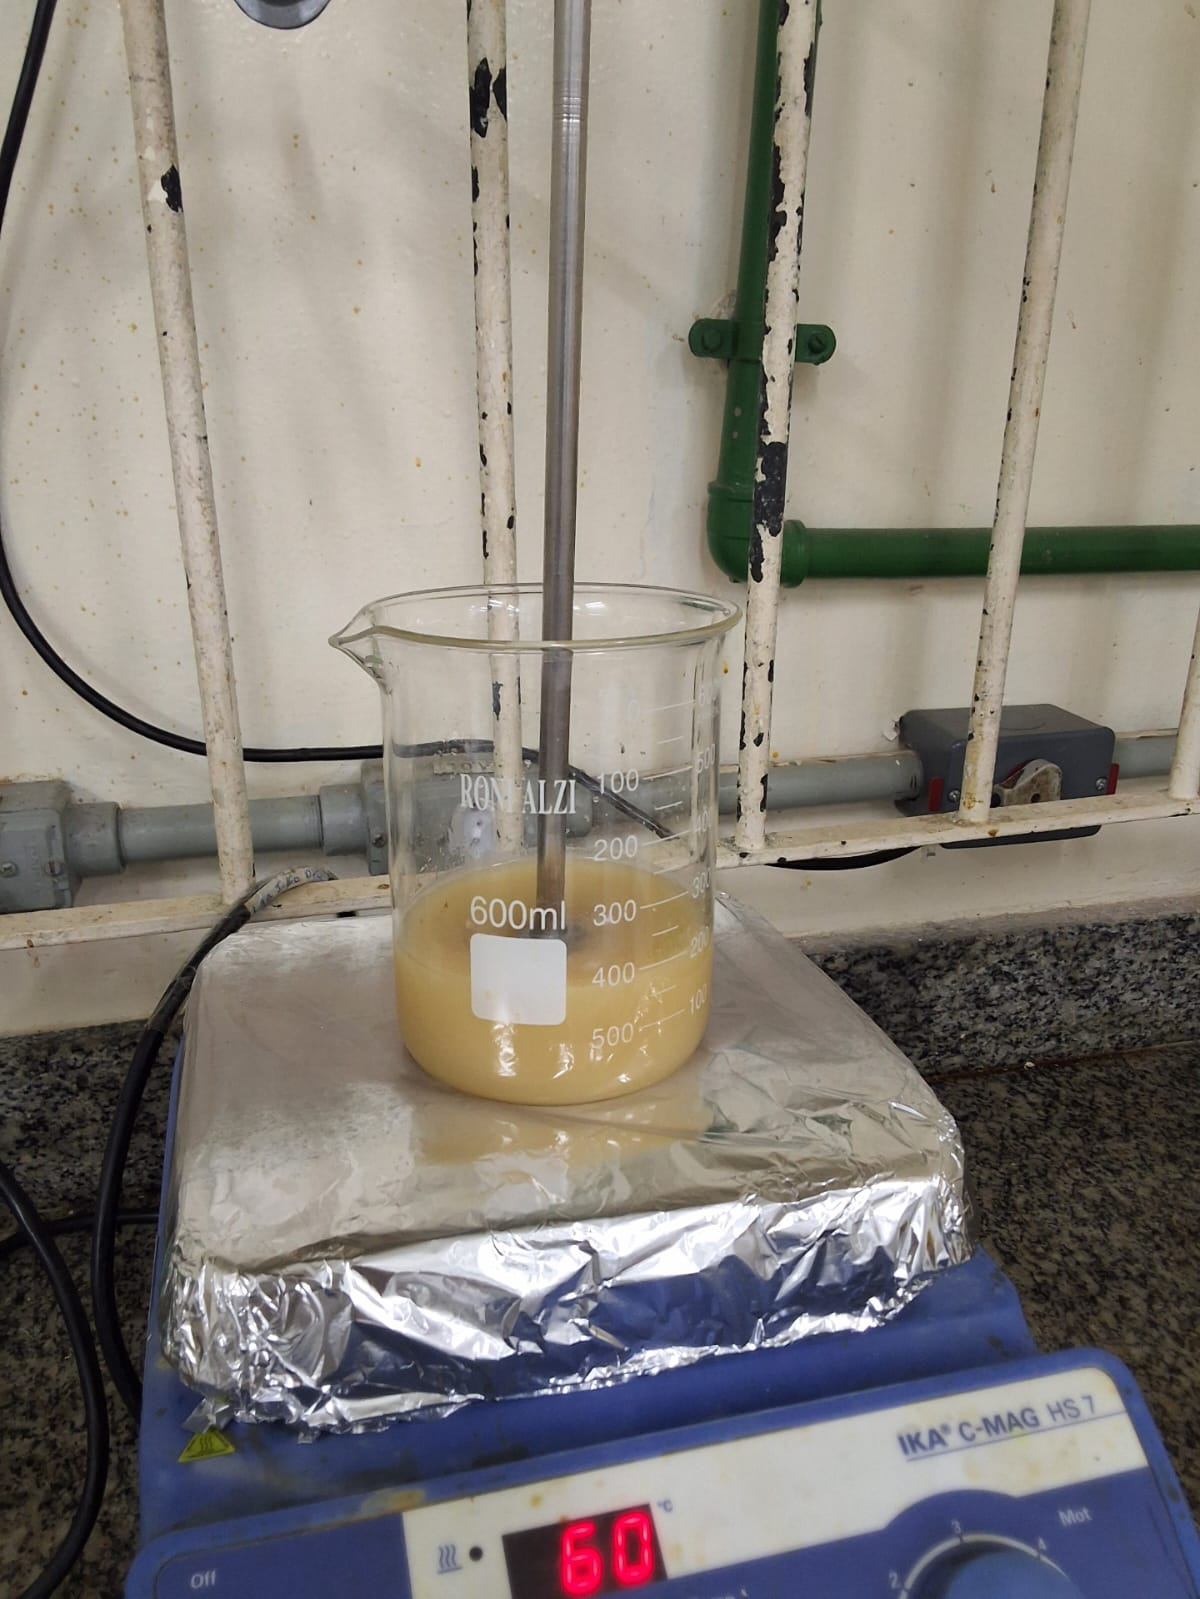
\includegraphics[width=0.4\textwidth]{src/fig/dia1/a1/inicio_recao.jpg}
    \caption{Amostra 1 do primeiro dia logo após a adição da solução básica.}
    \label{fig:dia1_a1_inicio}
\end{figure}

\begin{figure}[H]
    \centering
    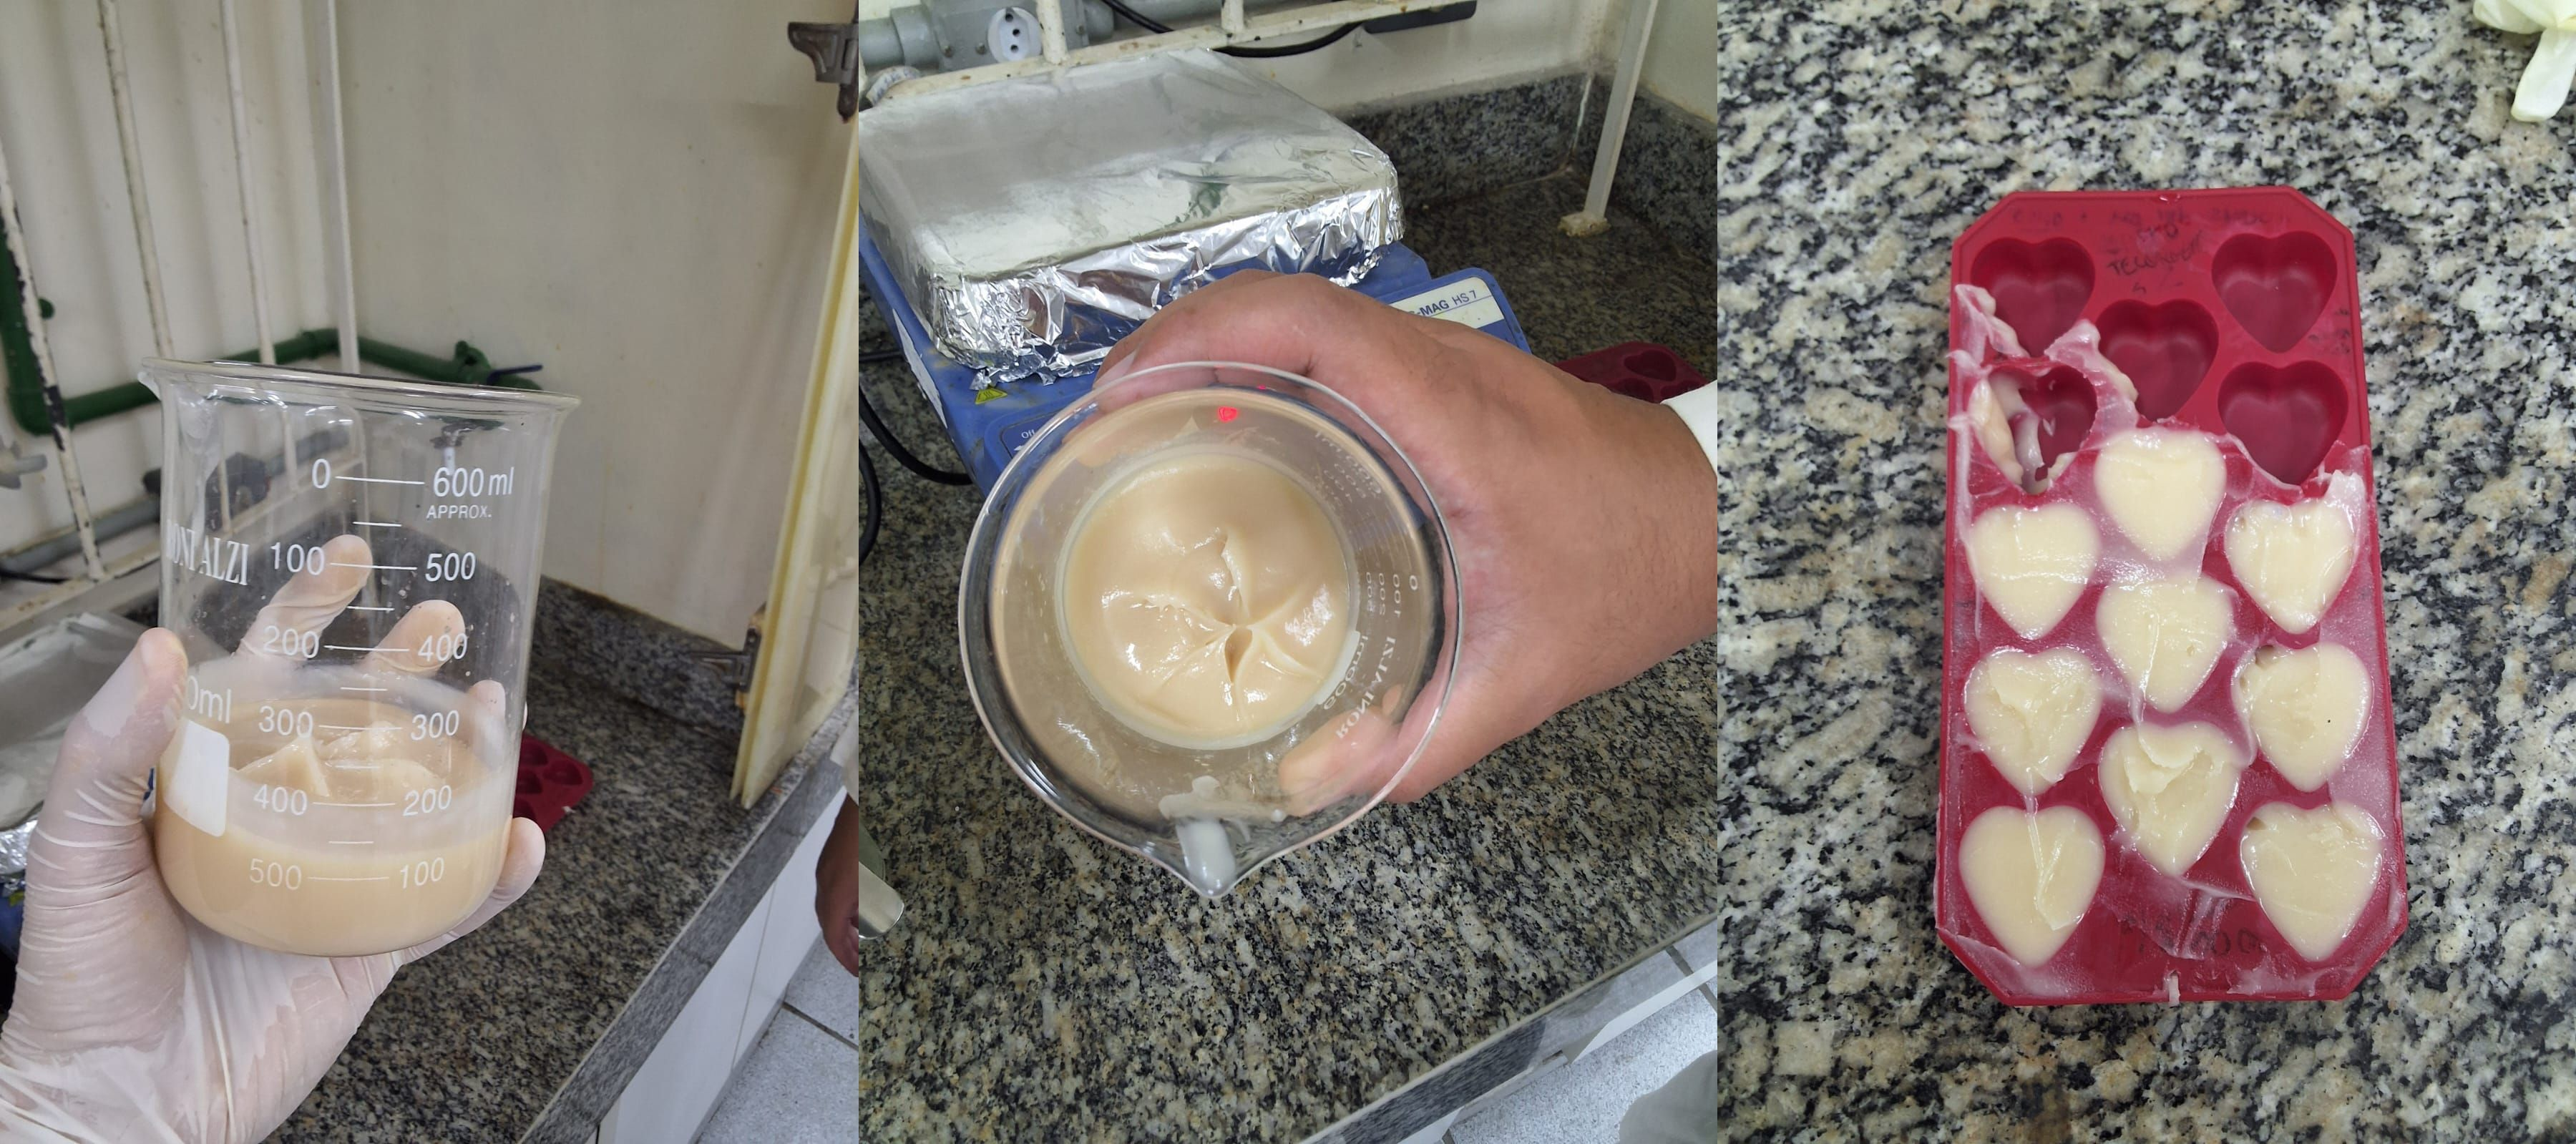
\includegraphics[width=0.8\textwidth]{src/fig/dia1/a1/final.jpg}
    \caption{Amostra 1 do primeiro dia ao final da etapa de bancada.}
    \label{fig:dia1_a1_final}
\end{figure}

\paragraph{Amostra 2.} A mistura de óleos da amostra~2 não foi tão bem proporcionada, resultando em 64,91\% de babaçu e 35,09\% de soja. Além disso, o excesso de base foi ainda mais acentuado: com o uso do babaçu, a quantidade ideal de NaOH seria de cerca de 19,07~g, mas foram utilizadas 20,12~g. Como a quantidade de base adicionada foi muito alta, a reação ocorreu praticamente de forma instantânea, em cerca de 25 segundos. Nesse intervalo, o sabão endureceu a ponto de o agitador, mesmo no nível~2, não conseguir mais se movimentar. Mediram-se pH~13 e temperatura interna de 75~°C, interrompendo-se então o aquecimento.

O produto resultante apresentou textura semelhante a areia molhada. Vale destacar que, em situações de excesso muito superior ao necessário, a reação pode ocorrer de maneira violenta, quase "explodindo" dentro do frasco e projetando sabão e óleo quente para os arredores.

\begin{figure}[H]
    \centering
    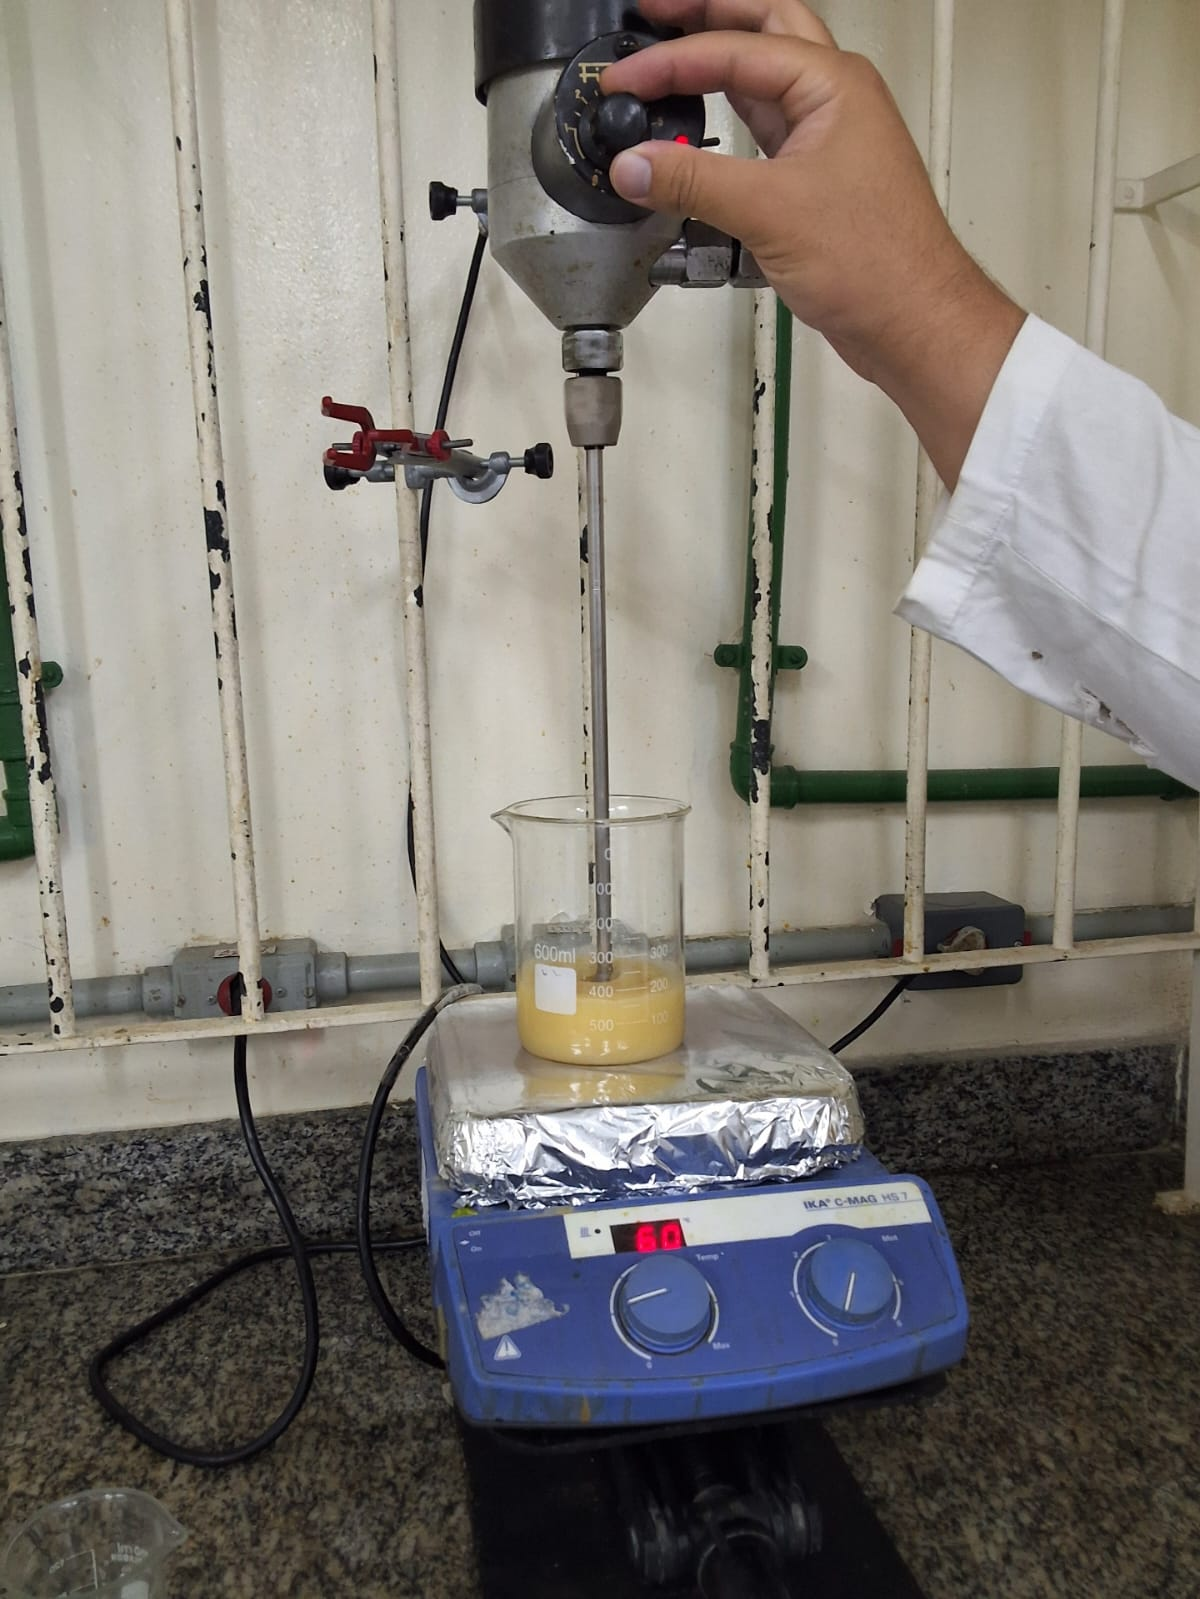
\includegraphics[width=0.4\textwidth]{src/fig/dia1/a2/inicio_reacao.jpg}
    \caption{Amostra 2 do primeiro dia logo após a adição da solução básica.}
    \label{fig:dia1_a2_inicio}
\end{figure}

\begin{figure}[H]
    \centering
    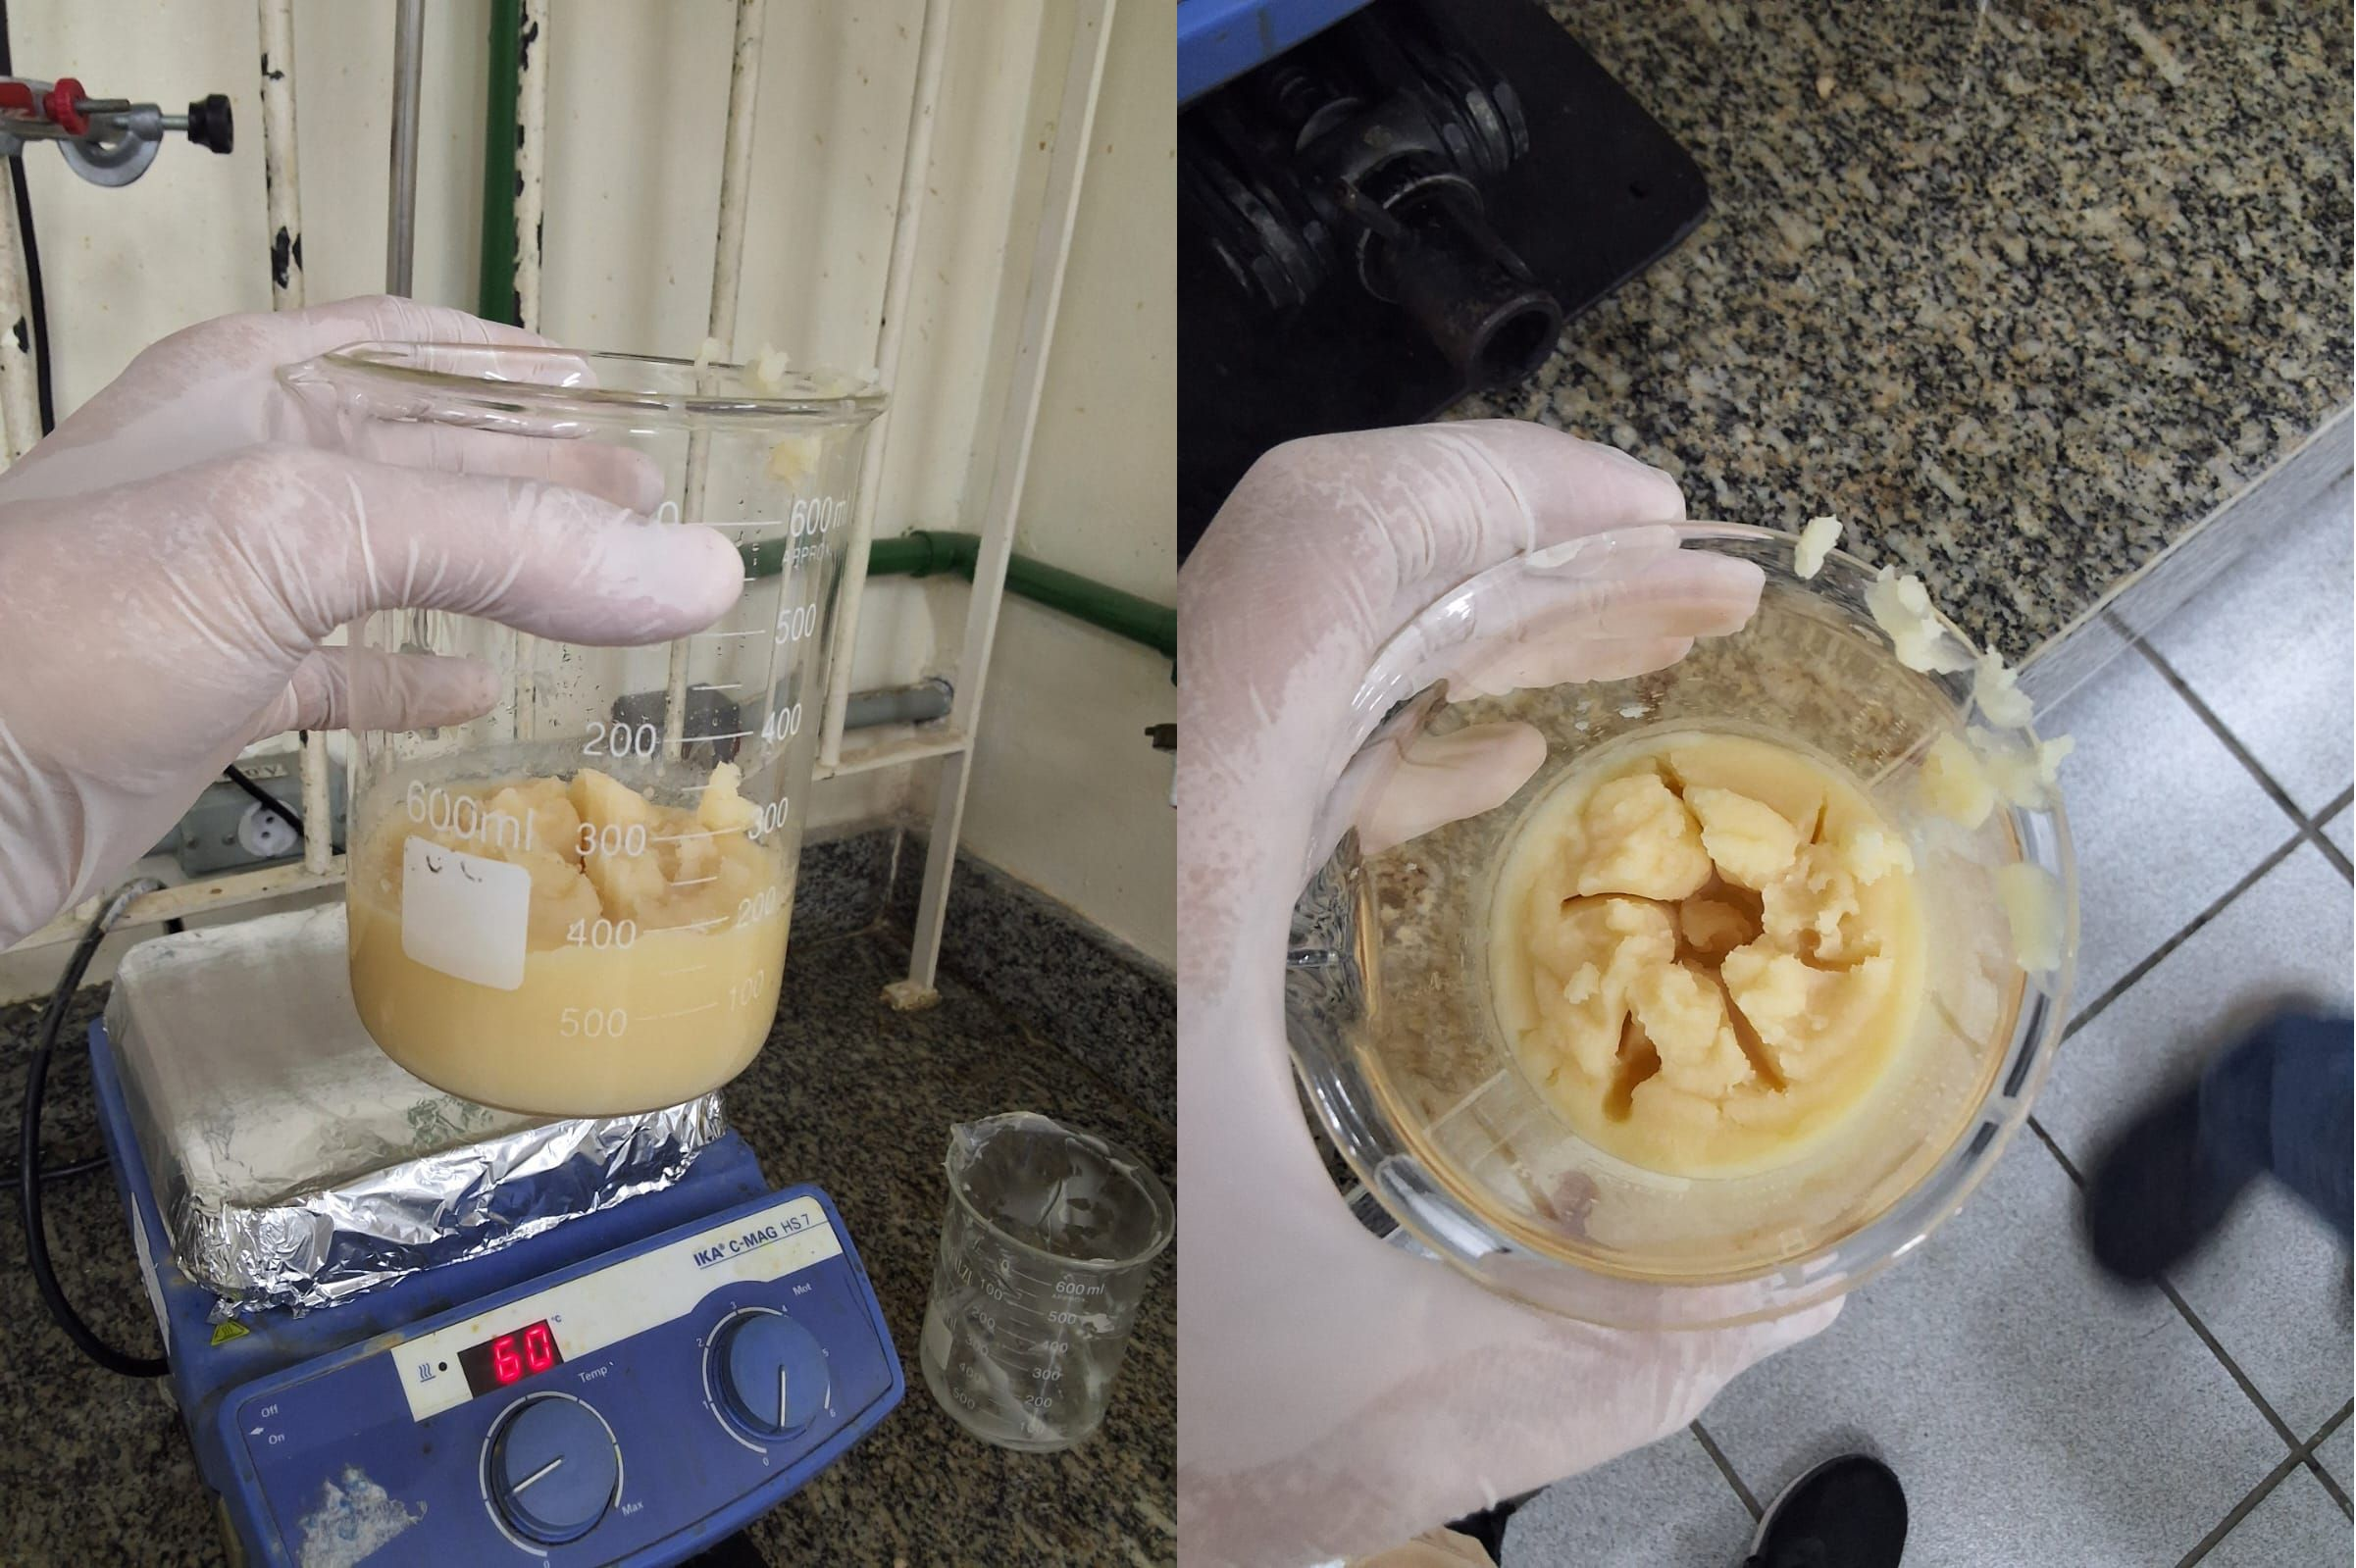
\includegraphics[width=0.6\textwidth]{src/fig/dia1/a2/final.jpg}
    \caption{Amostra 2 do primeiro dia ao final da etapa de bancada.}
    \label{fig:dia1_a2_final}
\end{figure}

\paragraph{Avaliação após a cura.} Após o período de cura, realizado ao longo da semana seguinte, as duas amostras foram avaliadas. A amostra~1 (cerca de 33\% de babaçu) apresentou consistência muito boa, com barras firmes e pH em torno de 10. Já a amostra~2 mostrou-se de qualidade ruim: a saponificação ocorreu rápido demais e de forma não homogênea, resultando em um sabão quebradiço e fragmentado, com pH~11. Esse contraste reforça o efeito do excesso de base discutido anteriormente.

\begin{figure}[H]
    \centering
    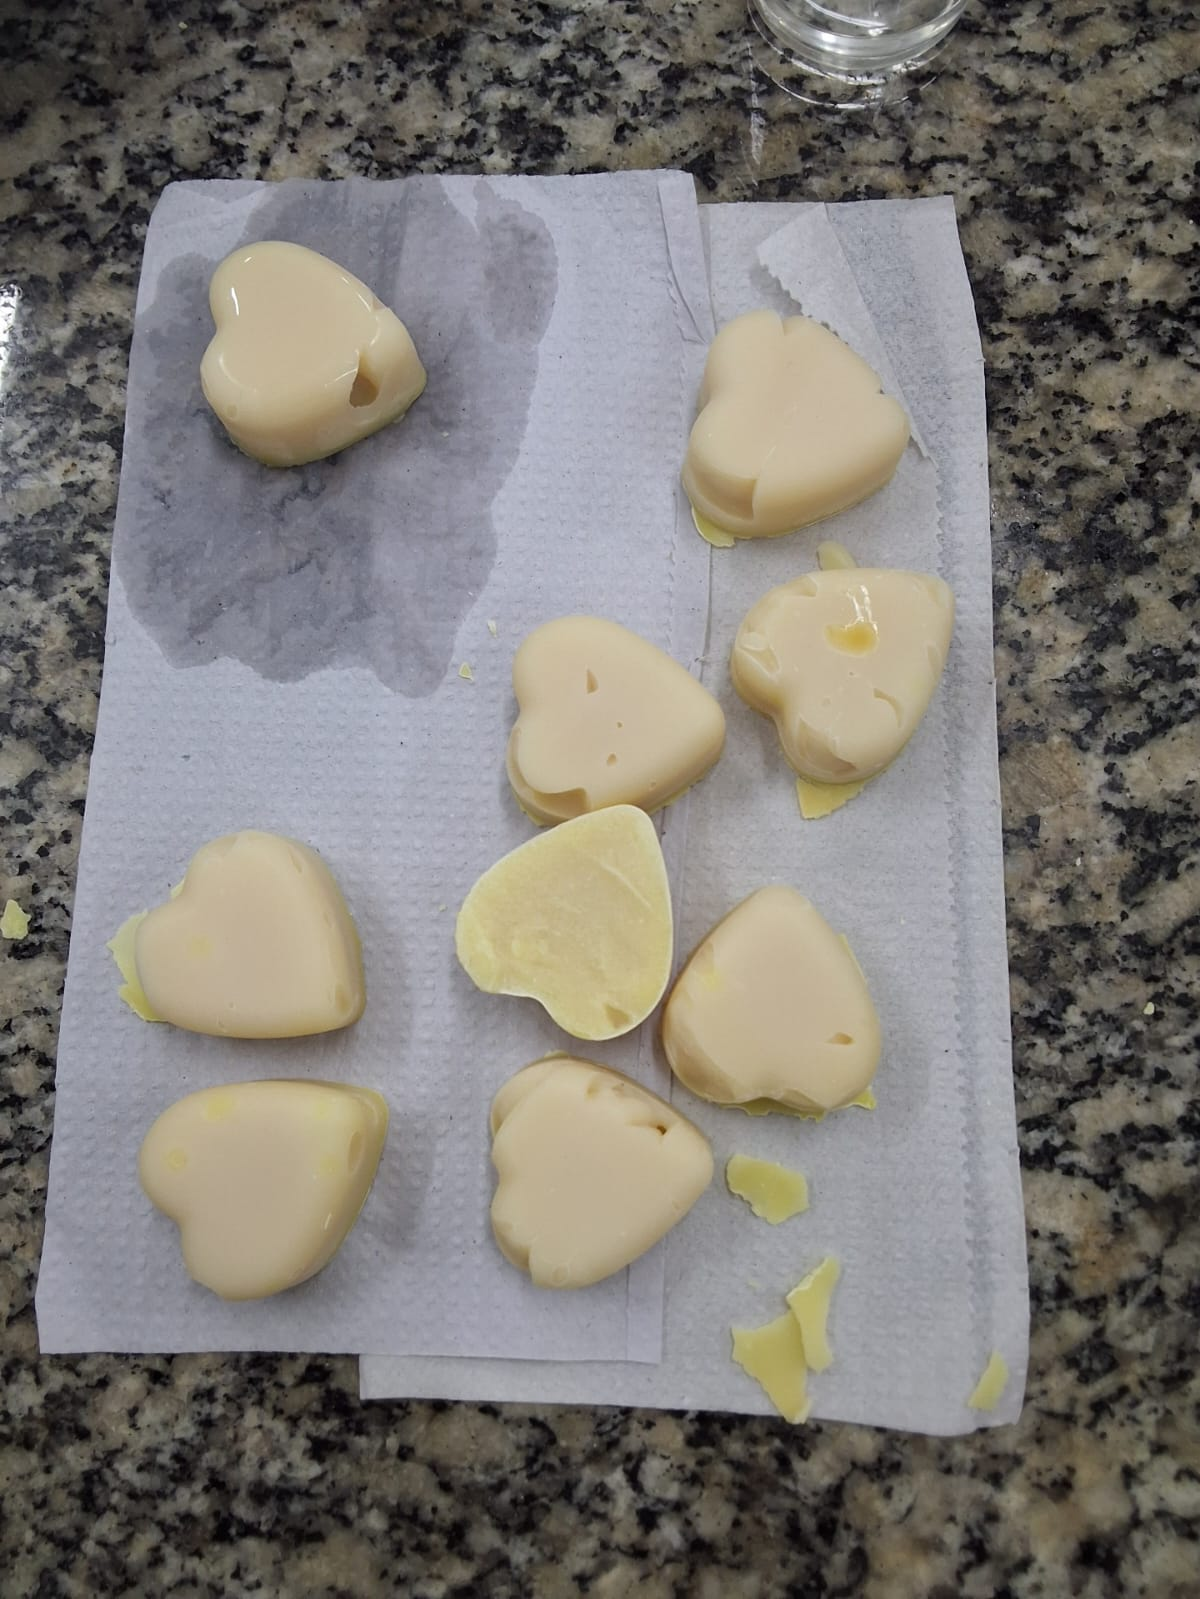
\includegraphics[width=0.4\textwidth]{src/fig/dia1/a1/resultado.jpg}
    \caption{Amostra 1 do primeiro dia após a cura.}
    \label{fig:dia1_a1_curado}
\end{figure}

\begin{figure}[H]
    \centering
    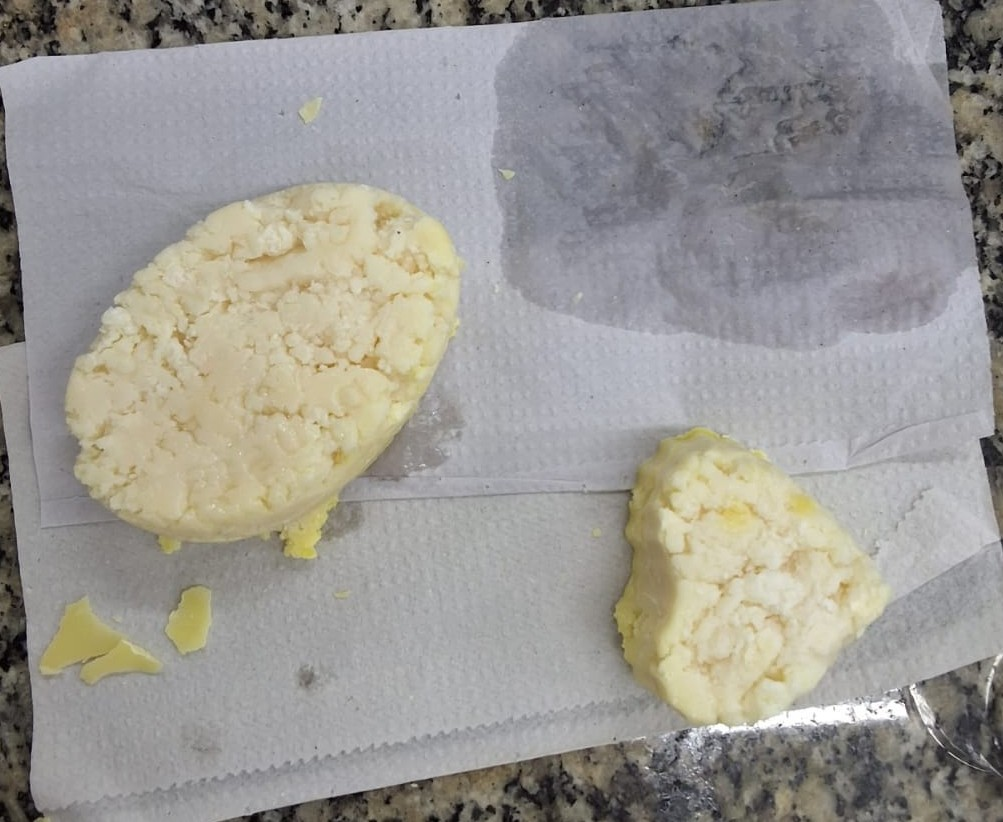
\includegraphics[width=0.4\textwidth]{src/fig/dia1/a2/resultado.jpg}
    \caption{Amostra 2 do primeiro dia após a cura.}
    \label{fig:dia1_a2_curado}
\end{figure}

\subsubsection{Segundo dia}

No segundo dia, o objetivo era novamente variar a composição da mistura de óleos. Tomando como referência o melhor resultado do primeiro dia, foram planejadas duas amostras, com o percentual de óleo de babaçu variado em $\pm$15\% em relação a essa referência e, novamente, sem a adição de ácido esteárico. As composições planejadas estão na Tabela~\ref{tab:dia2_planejado}.

\begin{table}[H]
    \centering
    \footnotesize
    \caption{Composição planejada para as amostras do segundo dia.}
    \label{tab:dia2_planejado}
    \begin{tabular}{ccccc}
        \toprule
        \textbf{Prática} & \textbf{P. babaçu (\%)} & \textbf{Massa de babaçu (g)} & \textbf{Massa de soja (g)} & \textbf{NaOH (g)} \\
        \midrule
        1 & 18 & 21,60 & 98,40 & 17,25 \\
        2 & 48 & 57,60 & 62,40 & 18,37 \\
        \bottomrule
    \end{tabular}
\end{table}

Durante a execução, a professora orientou que fosse produzida apenas uma amostra por dia, dado que o trabalho estava sendo realizado individualmente, e alertou que a quantidade de óleo de babaçu disponível poderia não ser suficiente para todos os experimentos previstos. Por esse motivo, optou-se por reduzir a massa total de cada amostra de 120~g para 80~g. Em razão dessa redução, o nível de óleo no becker ficou muito baixo, o que exigiu o uso de um termômetro culinário, já que um termômetro de mercúrio seria arriscado nessas condições.

Foi produzida apenas a amostra de menor percentual de babaçu (cerca de 18\%). A Tabela~\ref{tab:dia2_comparacao} compara os valores teóricos com os efetivamente realizados.

\begin{table}[H]
    \centering
    \footnotesize
    \caption{Comparação entre os valores teóricos e os realizados na amostra do segundo dia.}
    \label{tab:dia2_comparacao}
    \begin{tabular}{lcccc}
        \toprule
        & \textbf{P. babaçu (\%)} & \textbf{M. de babaçu (g)} & \textbf{M. de soja (g)} & \textbf{NaOH (g)} \\
        \midrule
        Teórico   & 18,00 & 14,40 & 65,60 & 11,50 \\
        Realizado & 17,81 & 15,56 & 71,81 & 11,50 \\
        \bottomrule
    \end{tabular}
\end{table}

Assim como nas demais amostras, utilizaram-se 30~ml de água na preparação da solução básica. Um ponto importante foi o uso de uma soda cáustica diferente da empregada no experimento anterior: dessa vez, uma soda em lascas, de coloração amarelada e aparentemente já contaminada por umidade — o que dificulta determinar a quantidade real de base reagindo.

Assim que a solução básica foi adicionada ao óleo, a mistura escureceu bastante e a viscosidade aumentou consideravelmente; nesse instante, o cronômetro foi iniciado (Figura~\ref{fig:dia2_inicio}). Com o passar do tempo, a mistura foi clareando, embora a viscosidade permanecesse praticamente constante (Figura~\ref{fig:dia2_momentos}). Aos 15 minutos, mediu-se um pH em torno de 12.

\begin{figure}[H]
    \centering
    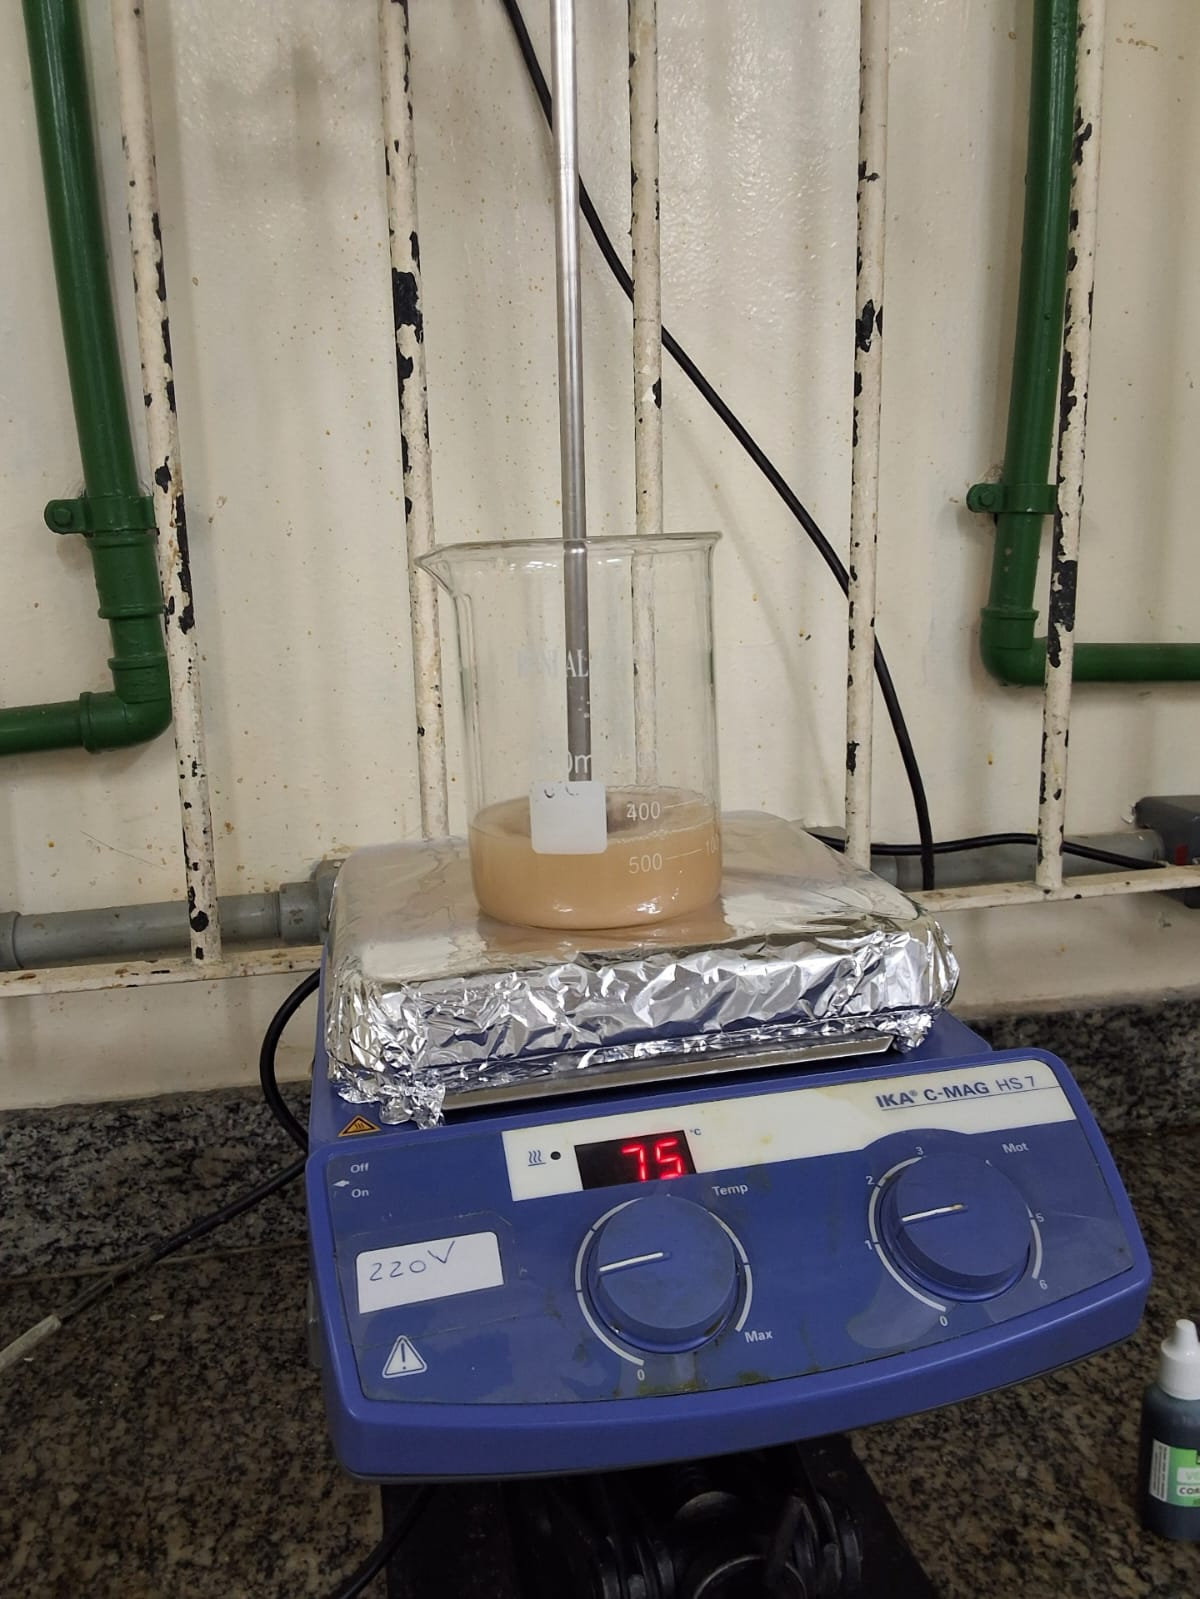
\includegraphics[width=0.4\textwidth]{src/fig/dia2/momento_1.jpg}
    \caption{Mistura do segundo dia logo após a adição da solução básica.}
    \label{fig:dia2_inicio}
\end{figure}

\begin{figure}[H]
    \centering
    \includegraphics[width=0.8\textwidth]{src/fig/dia2/momento_234.png}
    \caption{Evolução da mistura aos 10, 15 e 30 minutos de reação.}
    \label{fig:dia2_momentos}
\end{figure}

Diferentemente do primeiro dia, a quantidade de NaOH empregada foi a calculada para saponificar a mistura de babaçu e soja, e não a referente ao óleo de coco, que ainda constava como referência no planejamento. Como essa quantidade é menor, a reação ocorreu de forma bem mais lenta. Por esse motivo, aos 30 minutos, foram adicionados 1,28~g de NaOH, reajustando a quantidade de base ao nível previsto para o óleo de coco. Esse reajuste foi necessário porque, nesse mesmo dia, a proporção entre os óleos também havia sido alterada; sem ele, duas variáveis estariam sendo modificadas simultaneamente.

Após 45 minutos, a reação atingiu um estado satisfatório, ainda que com viscosidade abaixo do ideal, encerrando-se com pH~13. A coloração final apresentou-se bem mais escura, pois, aos 30 minutos, adicionou-se certa quantidade de corante verde; o resultado, contudo, não foi o esperado, e o material adquiriu tonalidade marrom-escura (Figura~\ref{fig:dia2_final}).

\begin{figure}[H]
    \centering
    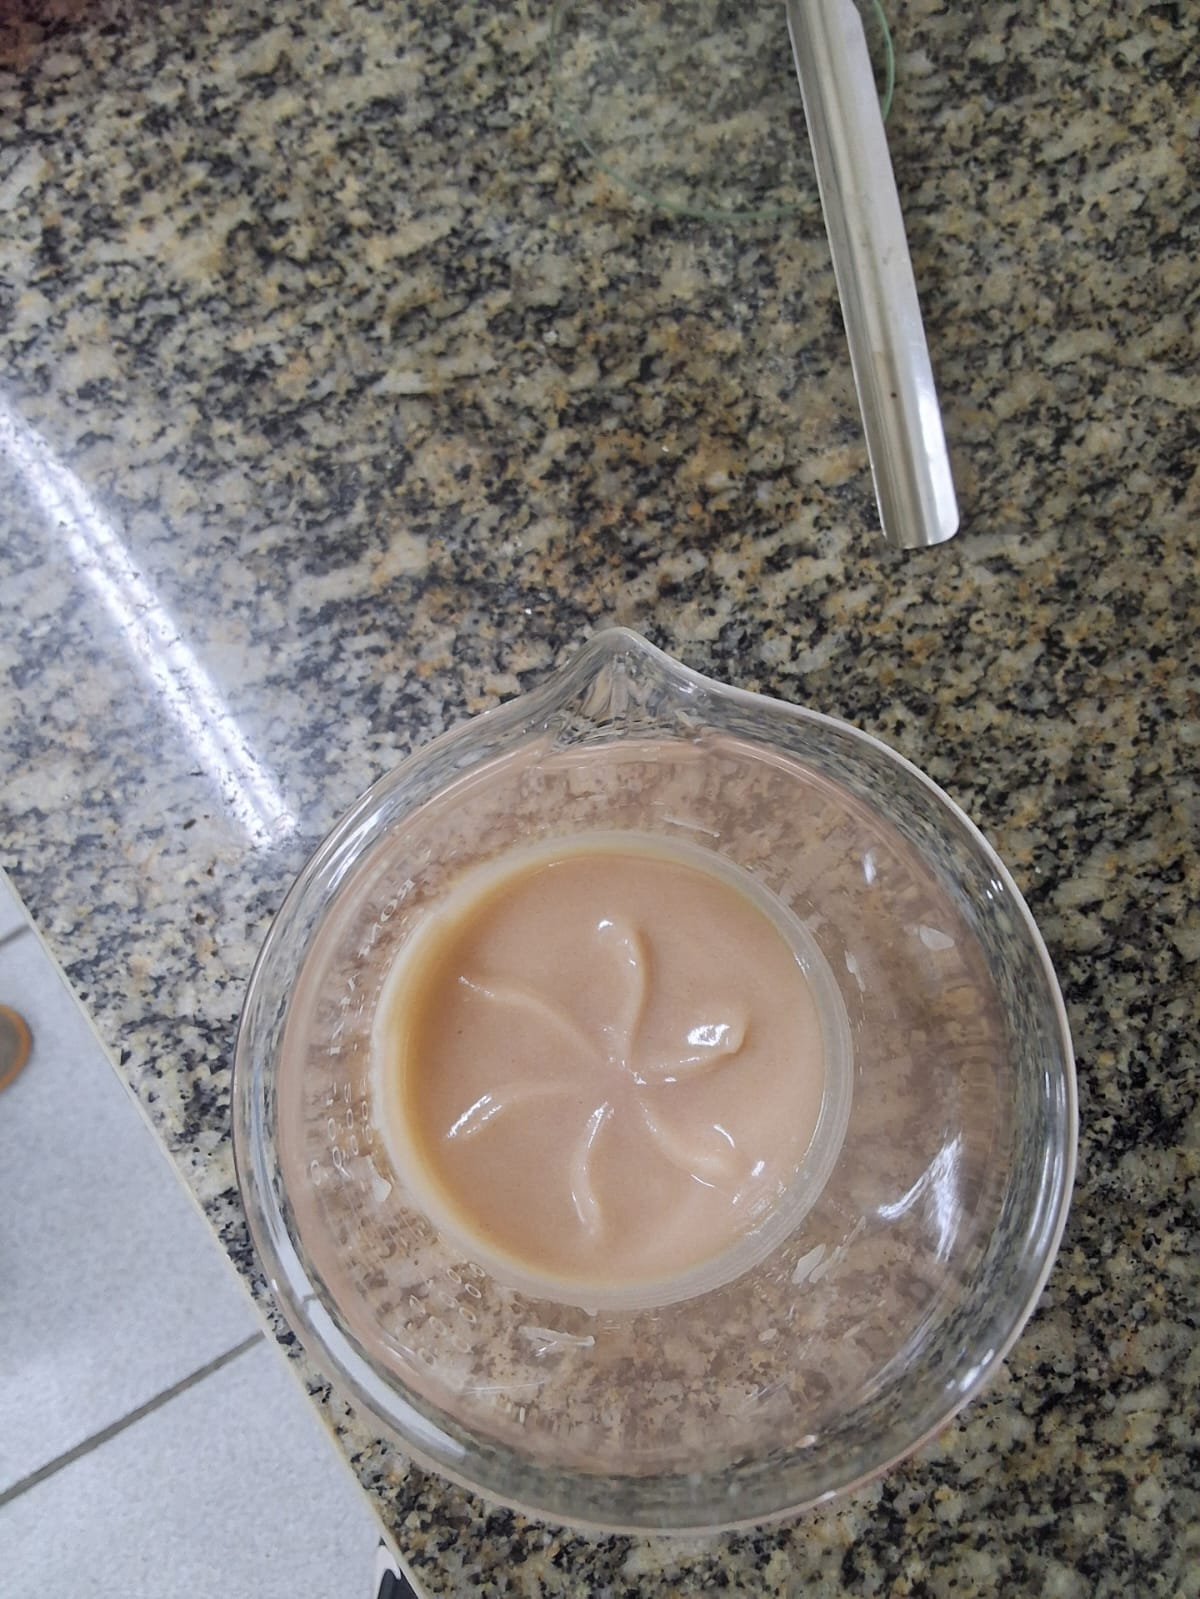
\includegraphics[width=0.4\textwidth]{src/fig/dia2/momento_5.jpg}
    \caption{Mistura do segundo dia ao final da etapa de bancada, após a adição de corante.}
    \label{fig:dia2_final}
\end{figure}

\subsubsection{Terceiro dia}

Definida a melhor mistura de óleos no primeiro dia, o objetivo do terceiro dia passou a ser identificar a melhor quantidade de ácido esteárico a ser adicionada, sem qualquer adição incremental de NaOH ao sistema. O planejamento previa o uso de ácido esteárico equivalente a 4\% da massa de óleo, conforme a Tabela~\ref{tab:dia3_planejado}.

\begin{table}[H]
    \centering
    \footnotesize
    \caption{Quantidade de ácido esteárico planejada para o terceiro dia.}
    \label{tab:dia3_planejado}
    \begin{tabular}{ccc}
        \toprule
        \textbf{Perc. de ác. (\%)} & \textbf{Massa total de óleo (g)} & \textbf{Massa de ác. esteárico (g)} \\
        \midrule
        10 & 120 & 4,8 \\
        \bottomrule
    \end{tabular}
\end{table}

O ácido esteárico foi introduzido a partir deste dia com dois objetivos. Por ser um ácido graxo saturado de cadeia longa (C18:0), ao reagir com o NaOH forma estearato de sódio, um sal que atua como agente estruturante, aumentando a dureza e a consistência da barra. Além disso, por consumir parte da base, espera-se que contribuísse para a redução do pH residual do produto. Diferentemente dos triglicerídeos, o ácido esteárico é um ácido graxo livre e reage diretamente com a base, conforme a Equação~\ref{eq:estearato}.

\begin{equation}
    \ce{C17H35COOH + NaOH -> C17H35COO^{-}Na^{+} + H2O}
    \label{eq:estearato}
\end{equation}

Por esse motivo, o ácido esteárico foi adicionado junto ao óleo, elevando-se a temperatura a cerca de 70~°C para a sua solubilização e retornando-se a 60~°C antes da adição da base.

No laboratório, após conversa com o monitor e o técnico, optou-se por reduzir a quantidade de ácido esteárico — da proporção planejada (4\%, ou 4,8~g) para cerca de 3\% da massa de óleo. Além disso, como o sabão produzido na semana anterior ainda não havia solidificado completamente, a única amostra com qualidade suficiente para servir de base foi a amostra~1 do primeiro dia (cerca de 33\% de babaçu). A Tabela~\ref{tab:dia3_comparacao} apresenta a composição-alvo e a efetivamente realizada; na coleta dos reagentes, empregou-se um pouco mais de ácido esteárico do que o planejado (cerca de 3,3\% da massa de óleo).

\begin{table}[H]
    \centering
    \footnotesize
    \caption{Composição-alvo e realizada na amostra do terceiro dia.}
    \label{tab:dia3_comparacao}
    \begin{tabular}{lcc}
        \toprule
        \textbf{Parâmetro} & \textbf{Alvo} & \textbf{Realizado} \\
        \midrule
        Massa de babaçu (g)        & 39,90  & 40,02  \\
        Massa de soja (g)          & 79,67  & 80,10  \\
        Massa total (g)            & 119,57 & 120,12 \\
        Perc. de babaçu (\%)       & 33,37  & 33,30  \\
        NaOH (g)                   & 18,48  & 18,52  \\
        Massa de ác. esteárico (g) & 3,58   & 3,98   \\
        \bottomrule
    \end{tabular}
\end{table}

Como nas demais práticas, a solução básica foi preparada com 30~ml de água (Figura~\ref{fig:dia3_naoh}). Antes da adição da base, o óleo foi aquecido e mantido em torno de 60~°C; ainda que a placa indicasse 80~°C, sua potência era constantemente ajustada para manter o óleo na temperatura desejada (Figura~\ref{fig:dia3_oleo}).

\begin{figure}[H]
    \centering
    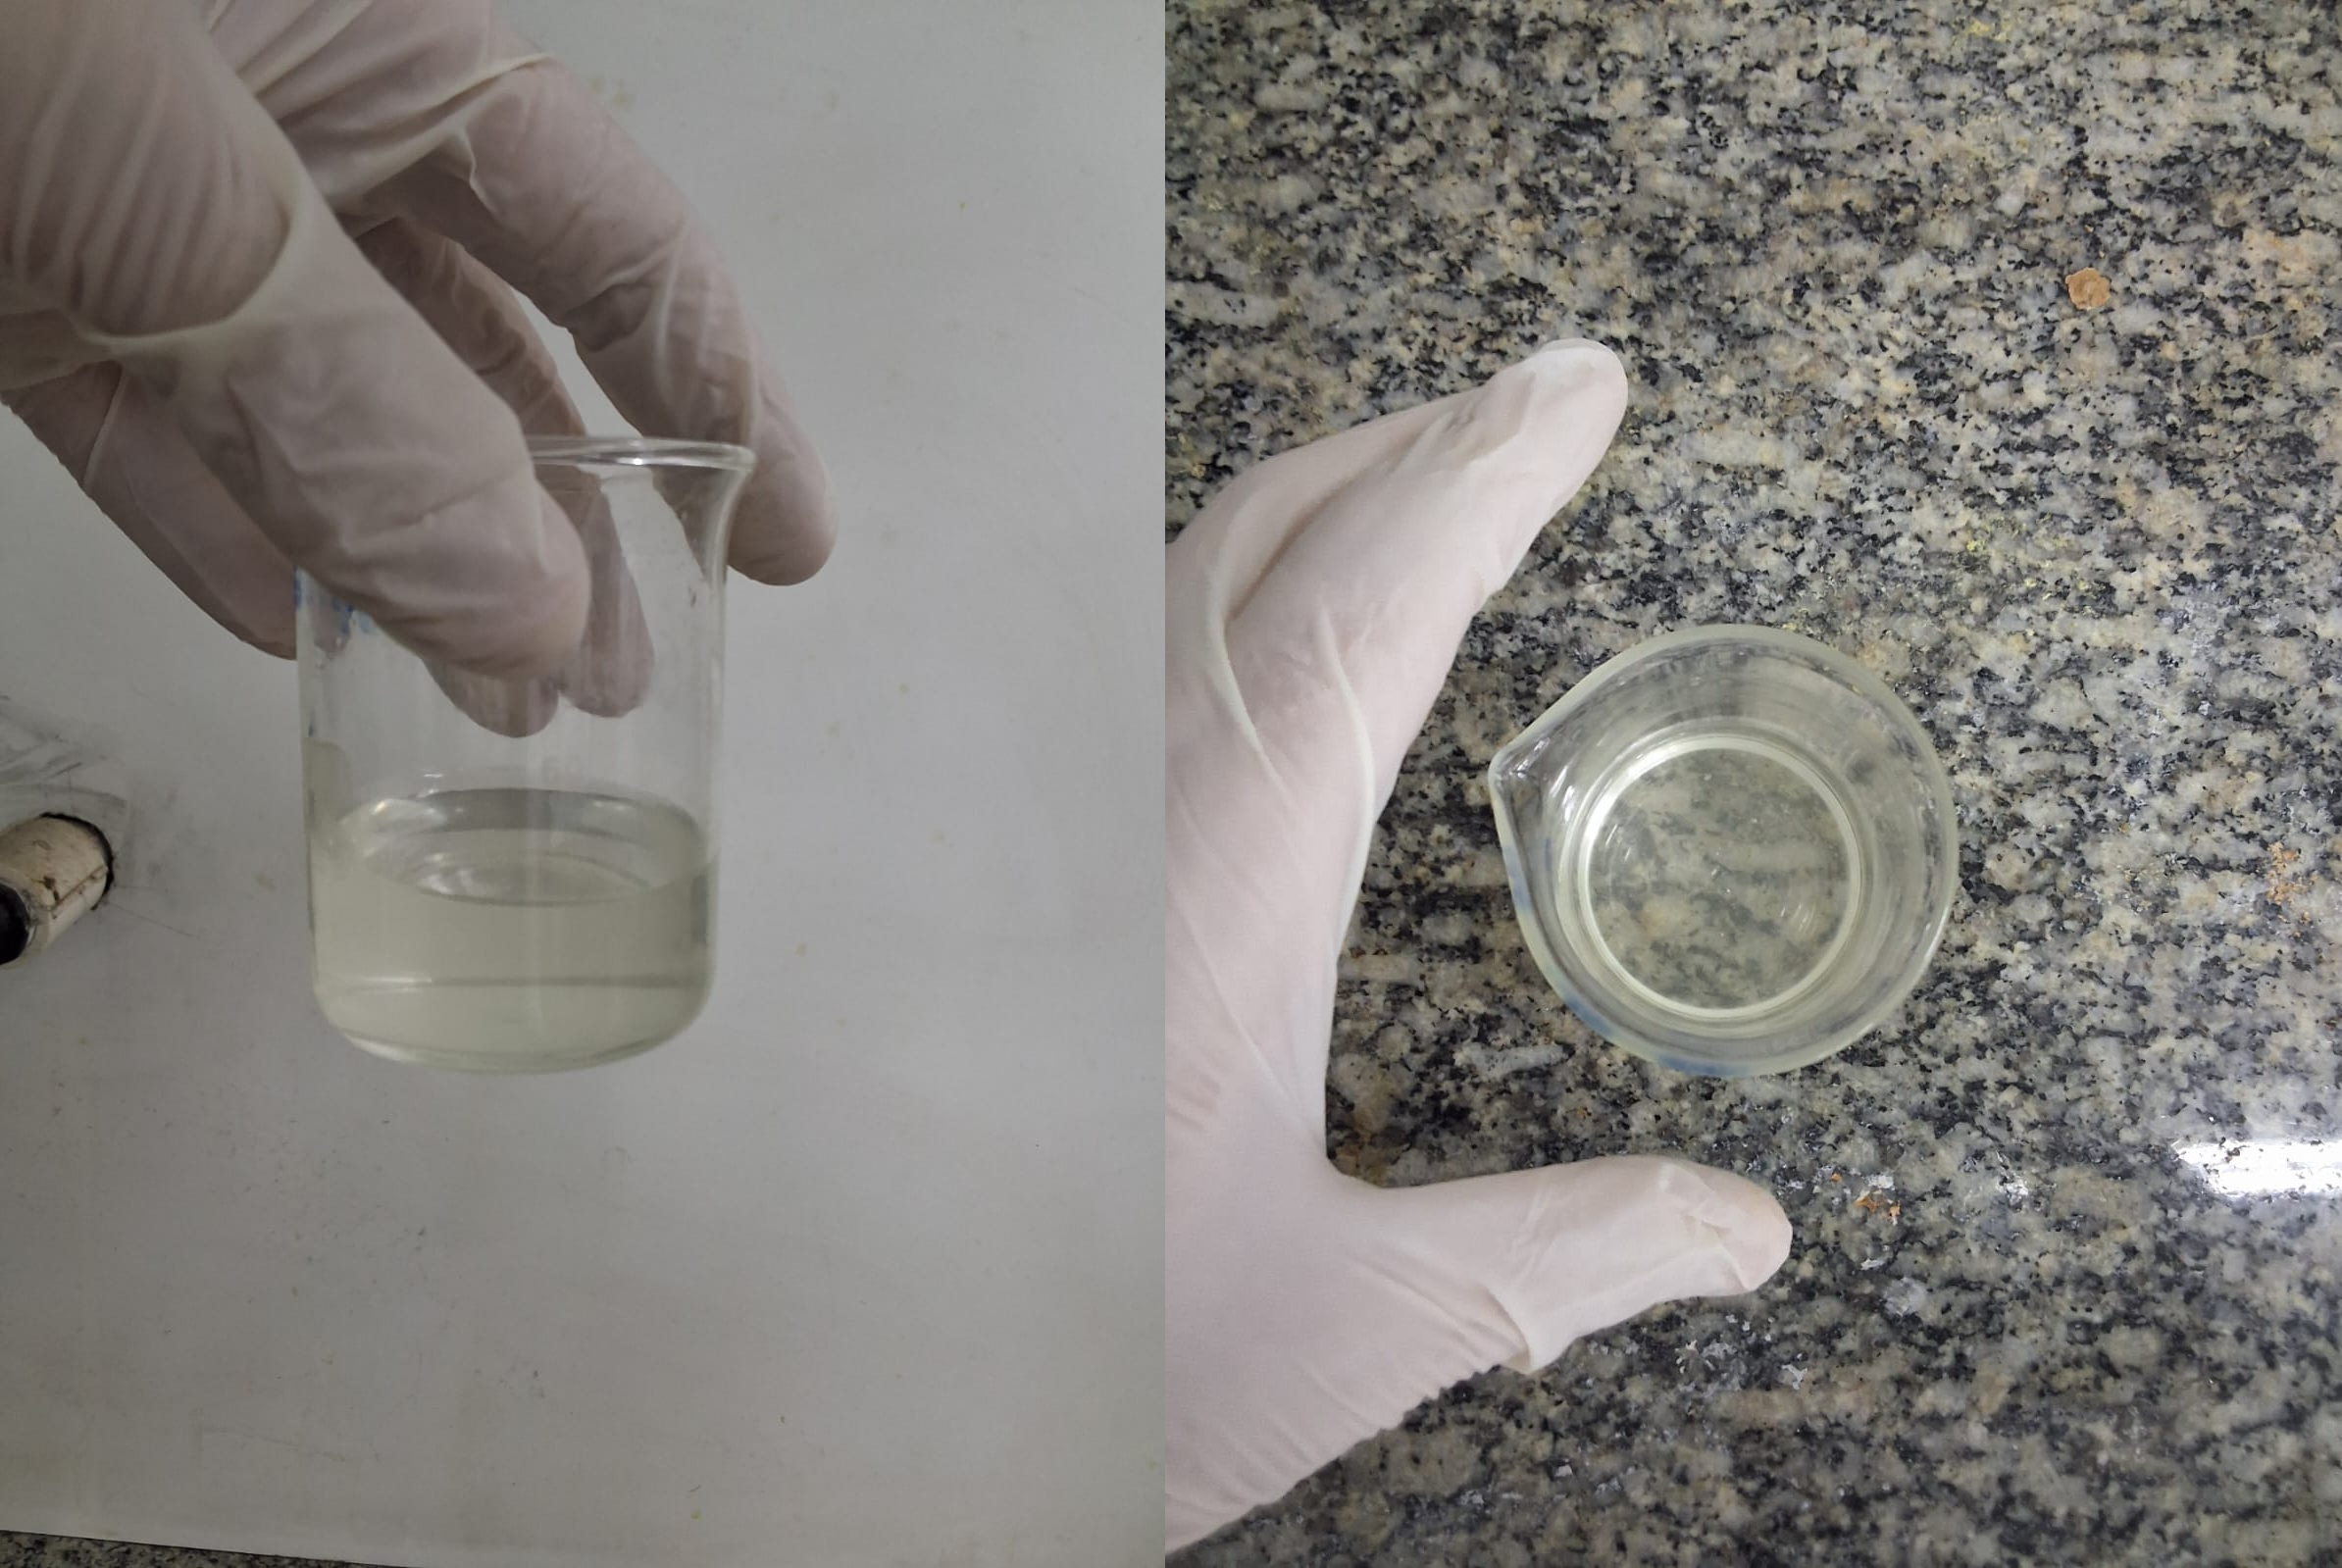
\includegraphics[width=0.8\textwidth]{src/fig/dia3/NaOH.png}
    \caption{Solução básica preparada no terceiro dia.}
    \label{fig:dia3_naoh}
\end{figure}

\begin{figure}[H]
    \centering
    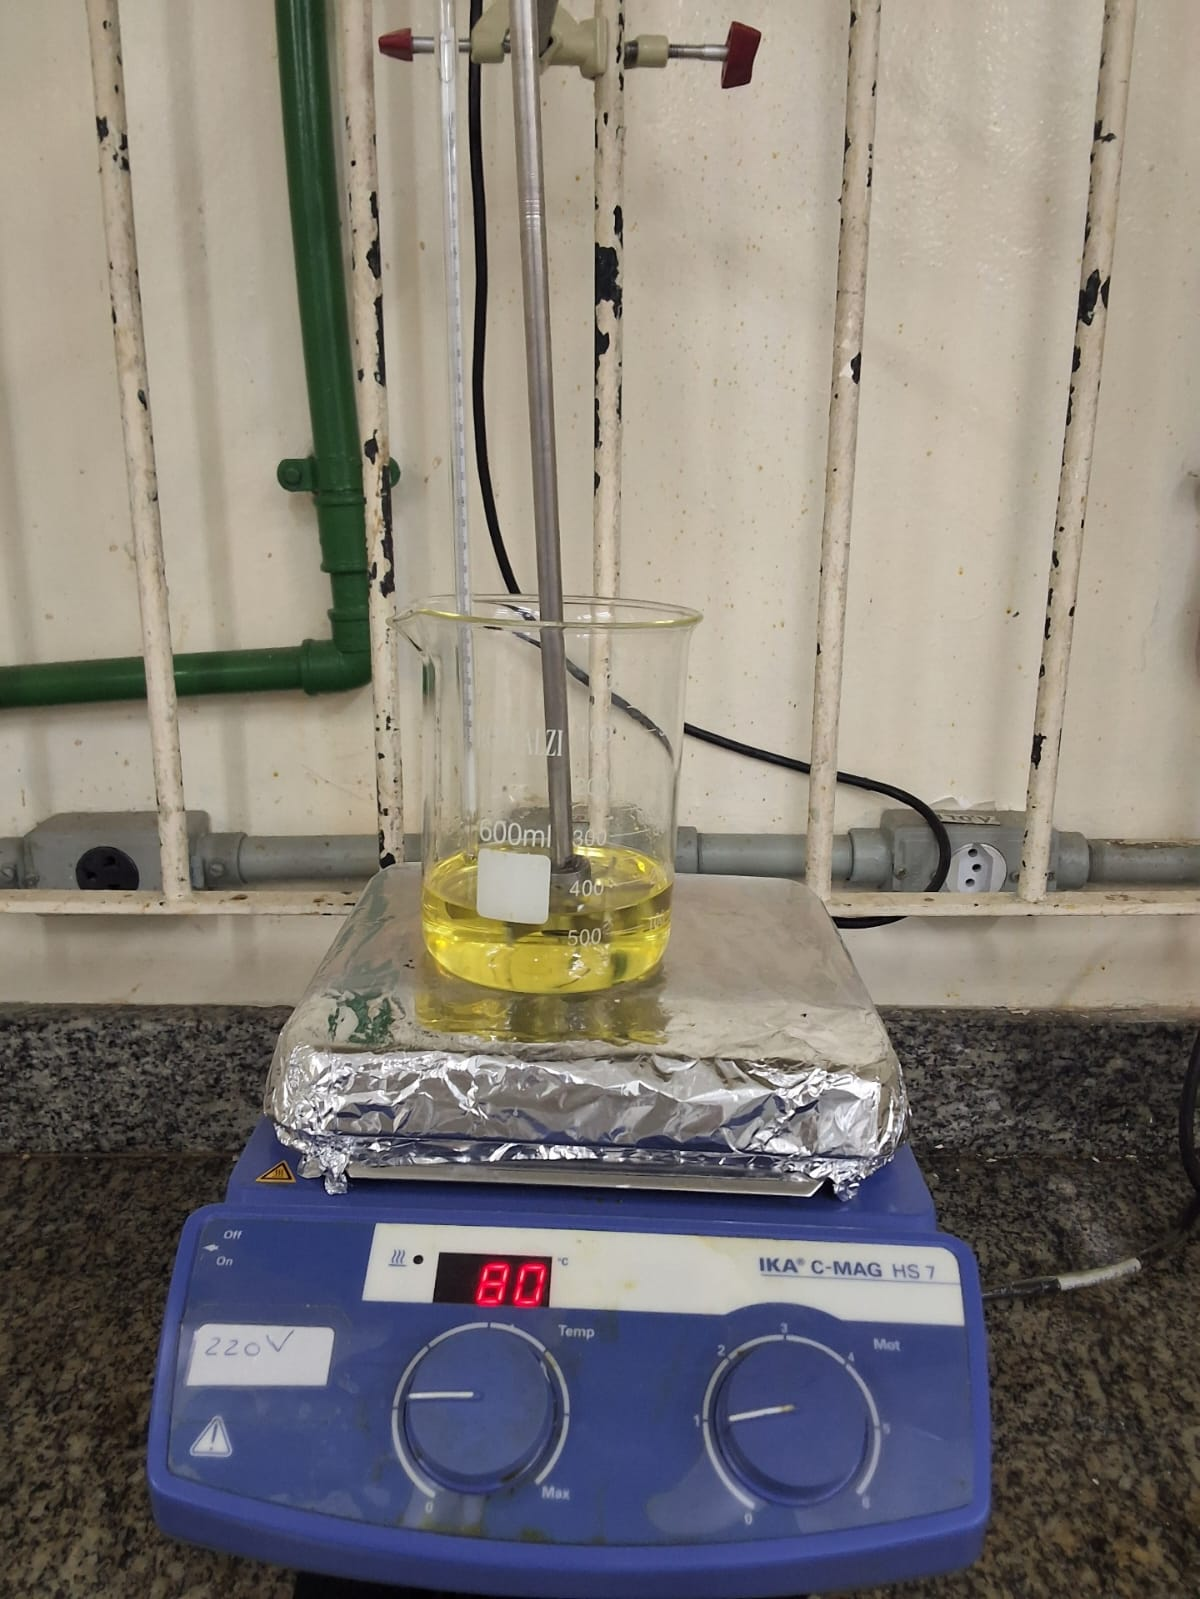
\includegraphics[width=0.4\textwidth]{src/fig/dia3/momento_0.jpg}
    \caption{Óleo mantido em torno de 60~°C antes da adição da base.}
    \label{fig:dia3_oleo}
\end{figure}

No momento em que a solução básica foi vertida no óleo, a mistura tornou-se muito viscosa, exigindo o ajuste imediato do agitador para a velocidade 1,5. Até os 4 minutos, a viscosidade aumentou ainda mais, elevando-se a velocidade para 2,5; a partir desse ponto, o aumento de viscosidade foi relativamente pequeno (Figura~\ref{fig:dia3_reacao}).

\begin{figure}[H]
    \centering
    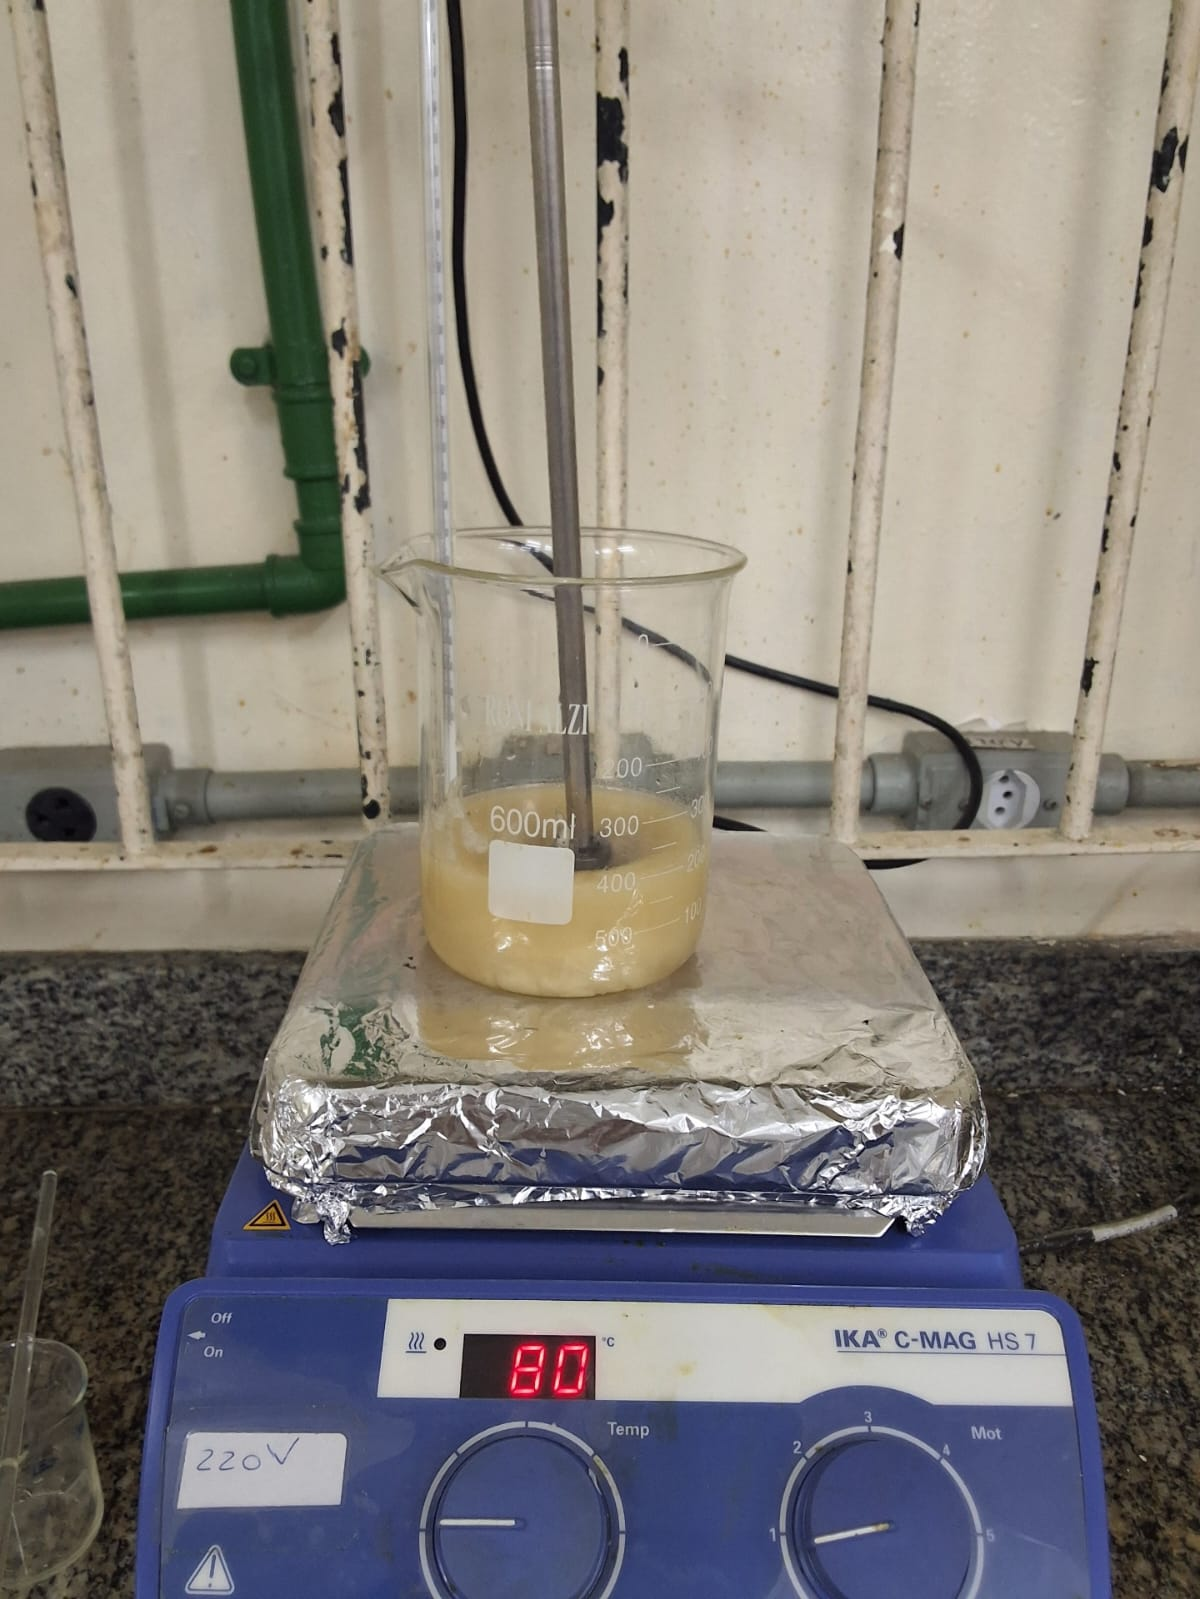
\includegraphics[width=0.4\textwidth]{src/fig/dia3/momento_1.jpg}
    \caption{Mistura do terceiro dia após a adição da solução básica.}
    \label{fig:dia3_reacao}
\end{figure}

Aos 14 minutos e 45 segundos, a viscosidade já exigia a velocidade 3 do agitador, razão pela qual a reação a quente foi interrompida e a massa foi transferida para os moldes. Não foi possível fotografar a pasta ainda no becker, devido ao risco de solidificação. A consistência obtida foi quase perfeita, muito semelhante a um purê de batatas (Figura~\ref{fig:dia3_final}).

\begin{figure}[H]
    \centering
    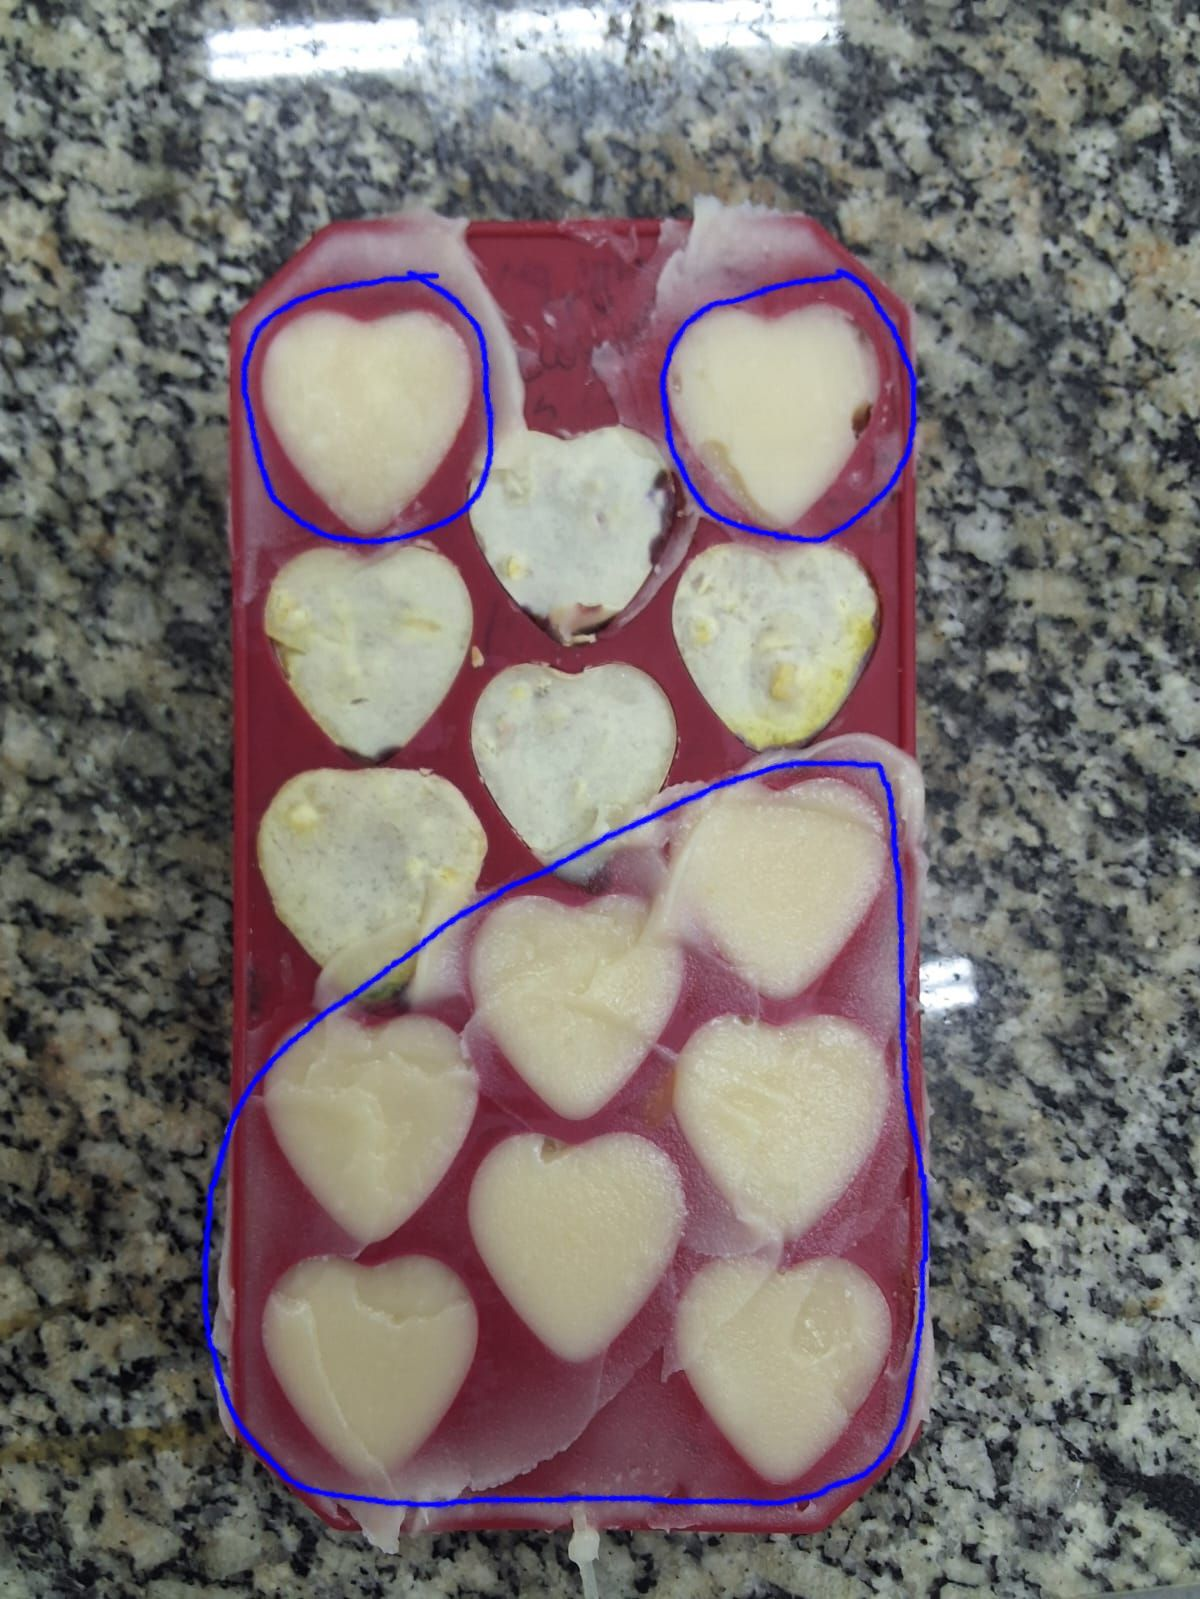
\includegraphics[width=0.4\textwidth]{src/fig/dia3/final.jpg}
    \caption{Amostra do terceiro dia ao final da etapa de bancada, nos moldes (corações destacados em azul); as demais peças, da semana anterior, ainda estavam moles.}
    \label{fig:dia3_final}
\end{figure}

\paragraph{Avaliação após a cura.} Esta foi a melhor amostra produzida até então. O efeito estruturante do ácido esteárico confirmou-se: a barra atingiu, com apenas uma semana de cura, a mesma firmeza que a amostra~1 do primeiro dia só havia alcançado após duas semanas. Quanto ao pH, contudo, não se observou redução notável no curto prazo, permanecendo em torno de 11 — de modo que o objetivo de reduzir o pH residual por meio do ácido esteárico não se mostrou efetivo neste experimento.

\subsubsection{Quarto dia}

Com o intuito de complementar o dia anterior, o objetivo do quarto dia seria validar se os dados obtidos no terceiro dia são bons o suficiente ou ainda podem melhorar. Como, no terceiro dia, a mistura ganhou viscosidade muito rapidamente, optou-se por reduzir a quantidade de ácido esteárico para 1,7\% da massa de óleo, conforme a Tabela~\ref{tab:dia4_planejado}.

\begin{table}[H]
    \centering
    \footnotesize
    \caption{Quantidade de ácido esteárico planejada para o quarto dia.}
    \label{tab:dia4_planejado}
    \begin{tabular}{ccc}
        \toprule
        \textbf{Perc. de ác. (\%)} & \textbf{Massa total de óleo (g)} & \textbf{Massa de ác. esteárico (g)} \\
        \midrule
        1,7 & 120 & 2,04 \\
        \bottomrule
    \end{tabular}
\end{table}

Manteve-se a mesma mistura de óleos definida como referência (cerca de 33\% de babaçu). A Tabela~\ref{tab:dia4_comparacao} apresenta a composição-alvo e a efetivamente realizada; empregou-se um pequeno excesso de soda cáustica em relação ao planejado (18,82~g, contra os 18,48~g previstos), sem maiores consequências.

\begin{table}[H]
    \centering
    \footnotesize
    \caption{Composição-alvo e realizada na amostra do quarto dia.}
    \label{tab:dia4_comparacao}
    \begin{tabular}{lcc}
        \toprule
        \textbf{Parâmetro} & \textbf{Alvo} & \textbf{Realizado} \\
        \midrule
        Massa de babaçu (g)        & 39,90  & 39,82  \\
        Massa de soja (g)          & 79,67  & 80,02  \\
        Massa total (g)            & 119,57 & 119,84 \\
        Perc. de babaçu (\%)       & 33,37  & 33,23  \\
        NaOH (g)                   & 18,48  & 18,82  \\
        Massa de ác. esteárico (g) & 2,04   & 2,04   \\
        \bottomrule
    \end{tabular}
\end{table}

Nesse dia, o óleo de soja utilizado nas práticas anteriores acabou, sendo necessário recorrer a um óleo de soja de outra marca (Figura~\ref{fig:dia4_oleo}). Assim como nos demais experimentos, a solução básica foi preparada com 30~ml de água (Figura~\ref{fig:dia4_naoh}).

\begin{figure}[H]
    \centering
    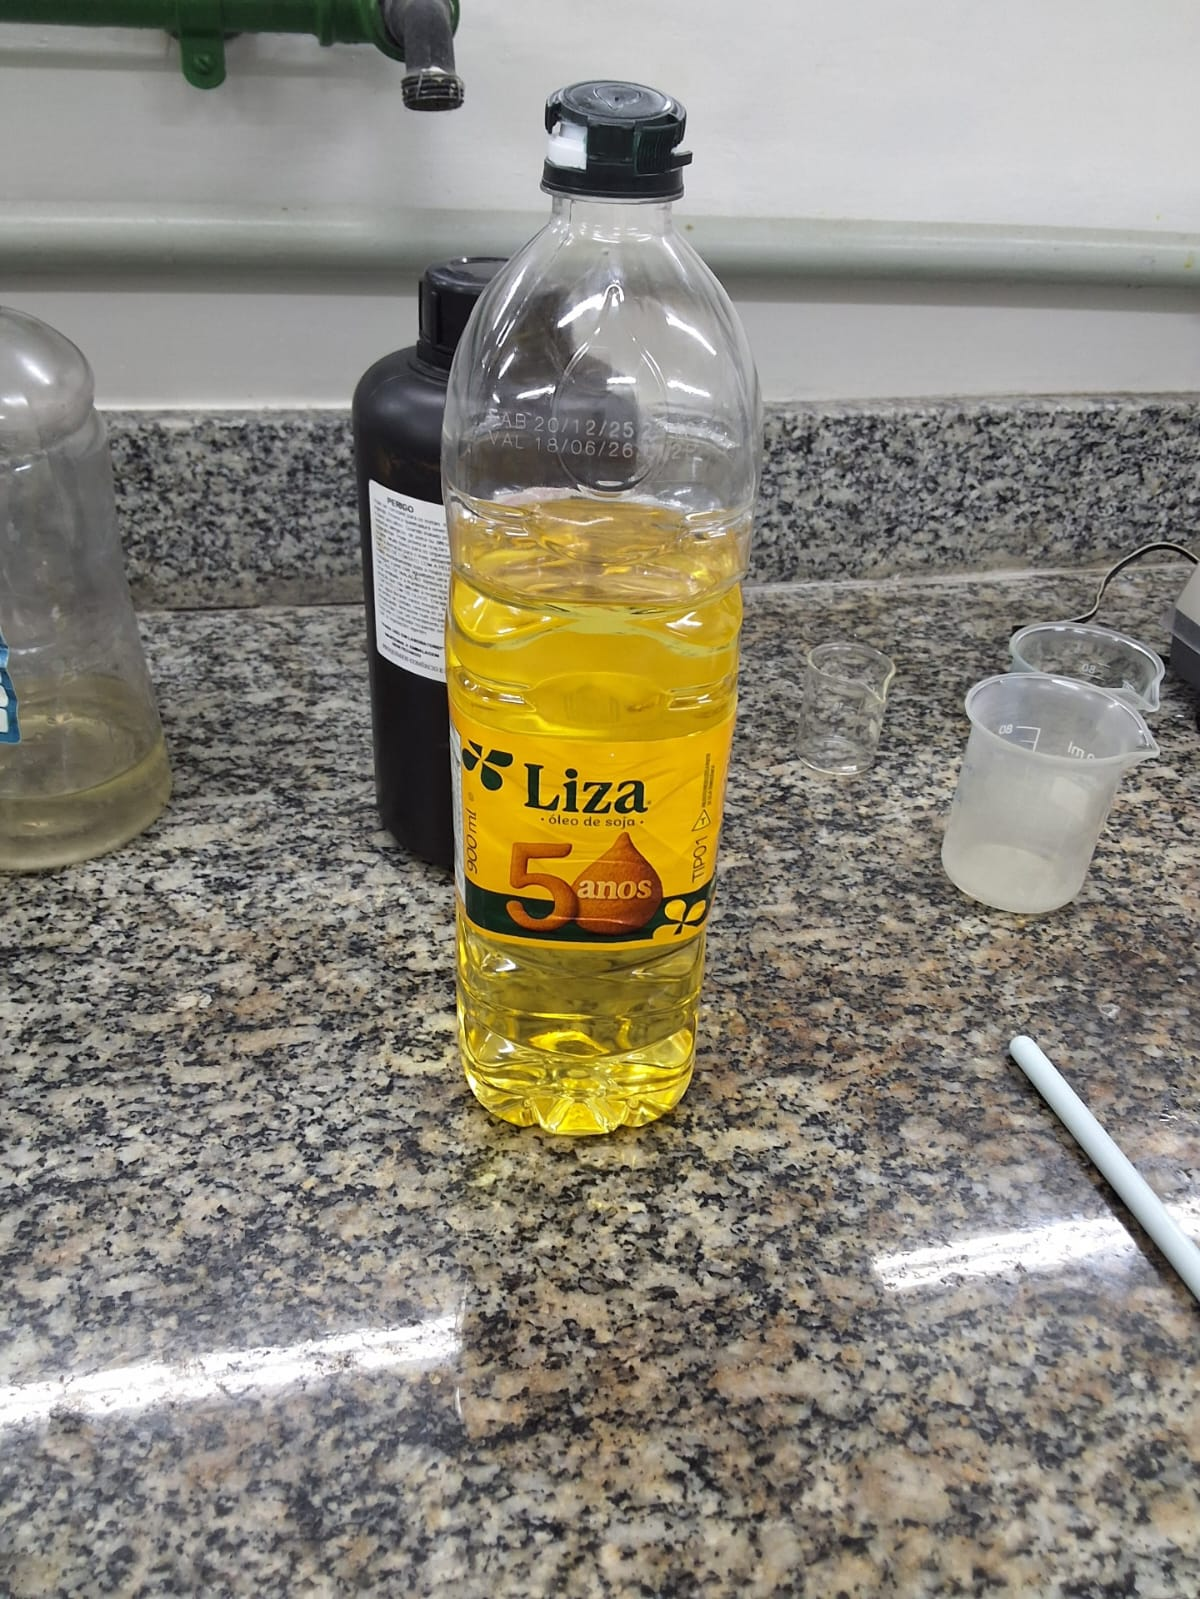
\includegraphics[width=0.4\textwidth]{src/fig/dia4/oleo.jpg}
    \caption{Óleo de soja de marca diferente, utilizado no quarto dia.}
    \label{fig:dia4_oleo}
\end{figure}

\begin{figure}[H]
    \centering
    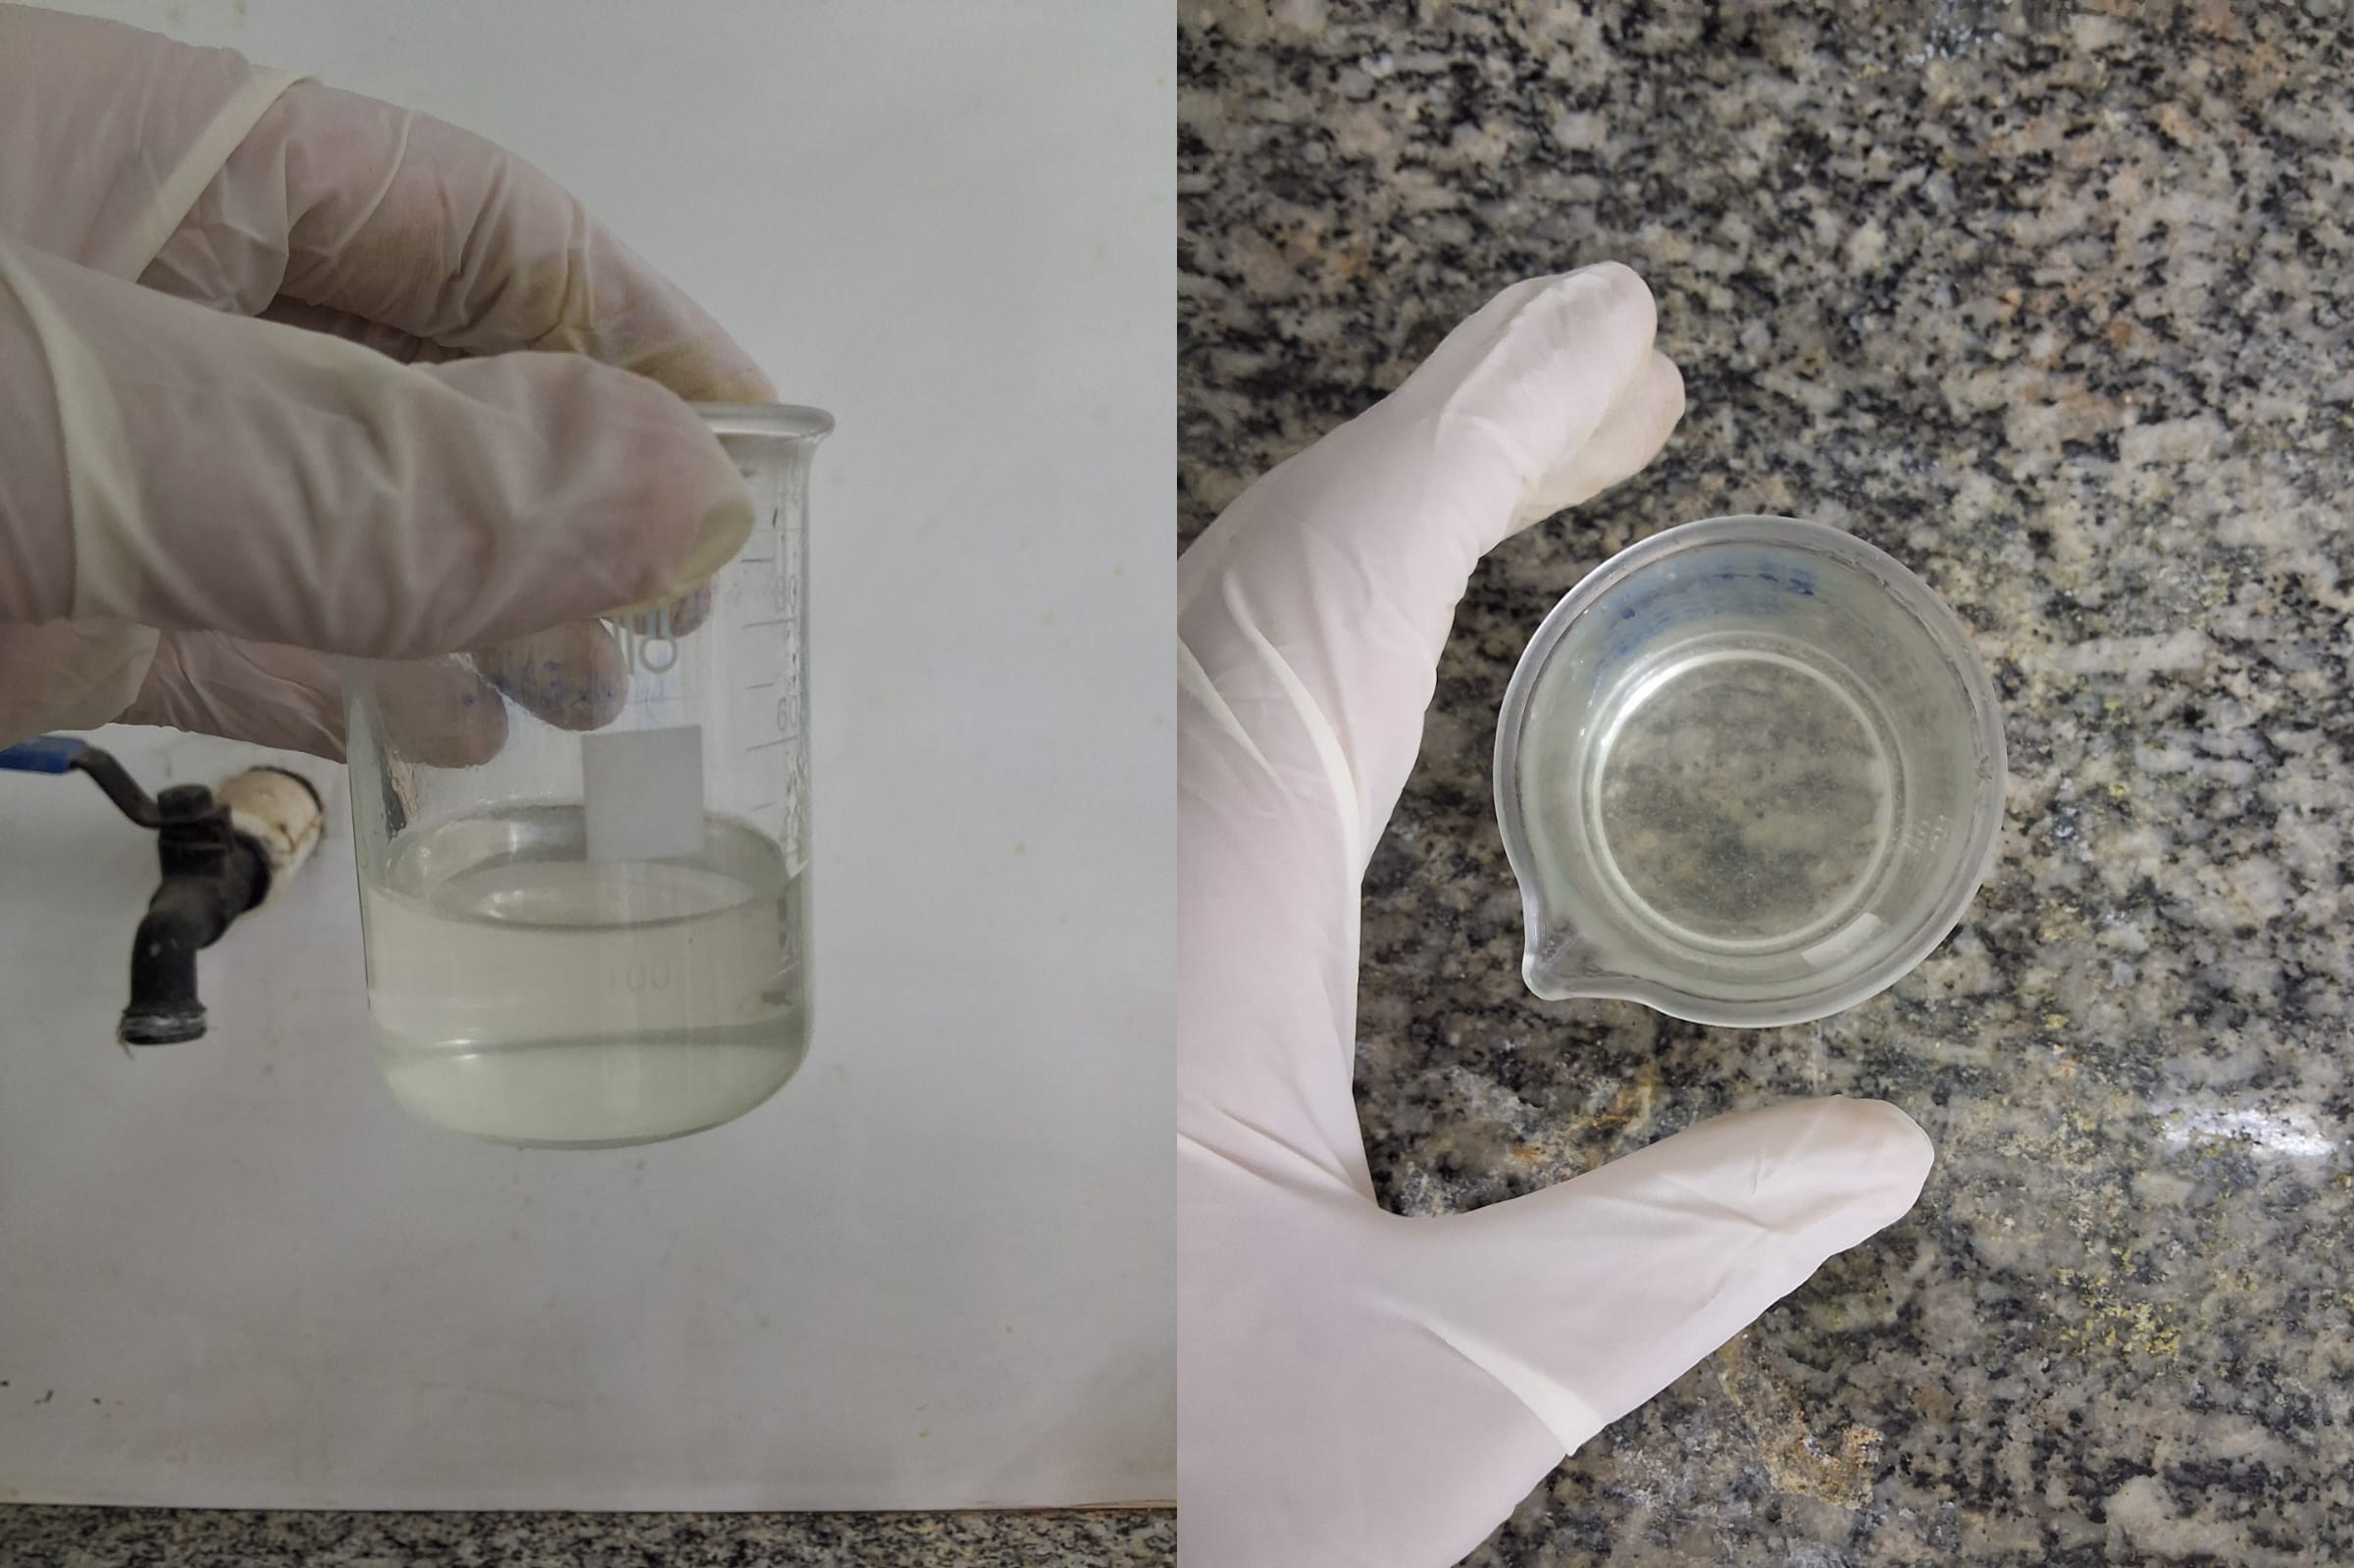
\includegraphics[width=0.8\textwidth]{src/fig/dia4/NaOH.png}
    \caption{Solução básica preparada no quarto dia.}
    \label{fig:dia4_naoh}
\end{figure}

Antes da adição da solução básica, o óleo foi superaquecido a mais de 110~°C por engano. A intenção era apenas solubilizar o ácido esteárico, mas a falta de atenção levou ao descuido com a temperatura. Embora não tenha inviabilizado a amostra, esse tipo de superaquecimento é justamente o que pode gerar ácidos graxos livres (AGLs) por degradação térmica, ainda que de forma mínima. Após a redução da temperatura para cerca de 60~°C e a sua estabilização — mantida na faixa de 60 a 63~°C por um período de 4 minutos —, prosseguiu-se com o experimento.

Com a adição da base ao óleo, a temperatura subiu para 65~°C e a viscosidade aumentou notoriamente (Figura~\ref{fig:dia4_inicio}). Dessa vez, o aumento de viscosidade foi bem mais gradual, aproximando-se do ponto de viscosidade ideal aos 14 minutos, a 55~°C e com pH~13 (Figura~\ref{fig:dia4_ponto}).

\begin{figure}[H]
    \centering
    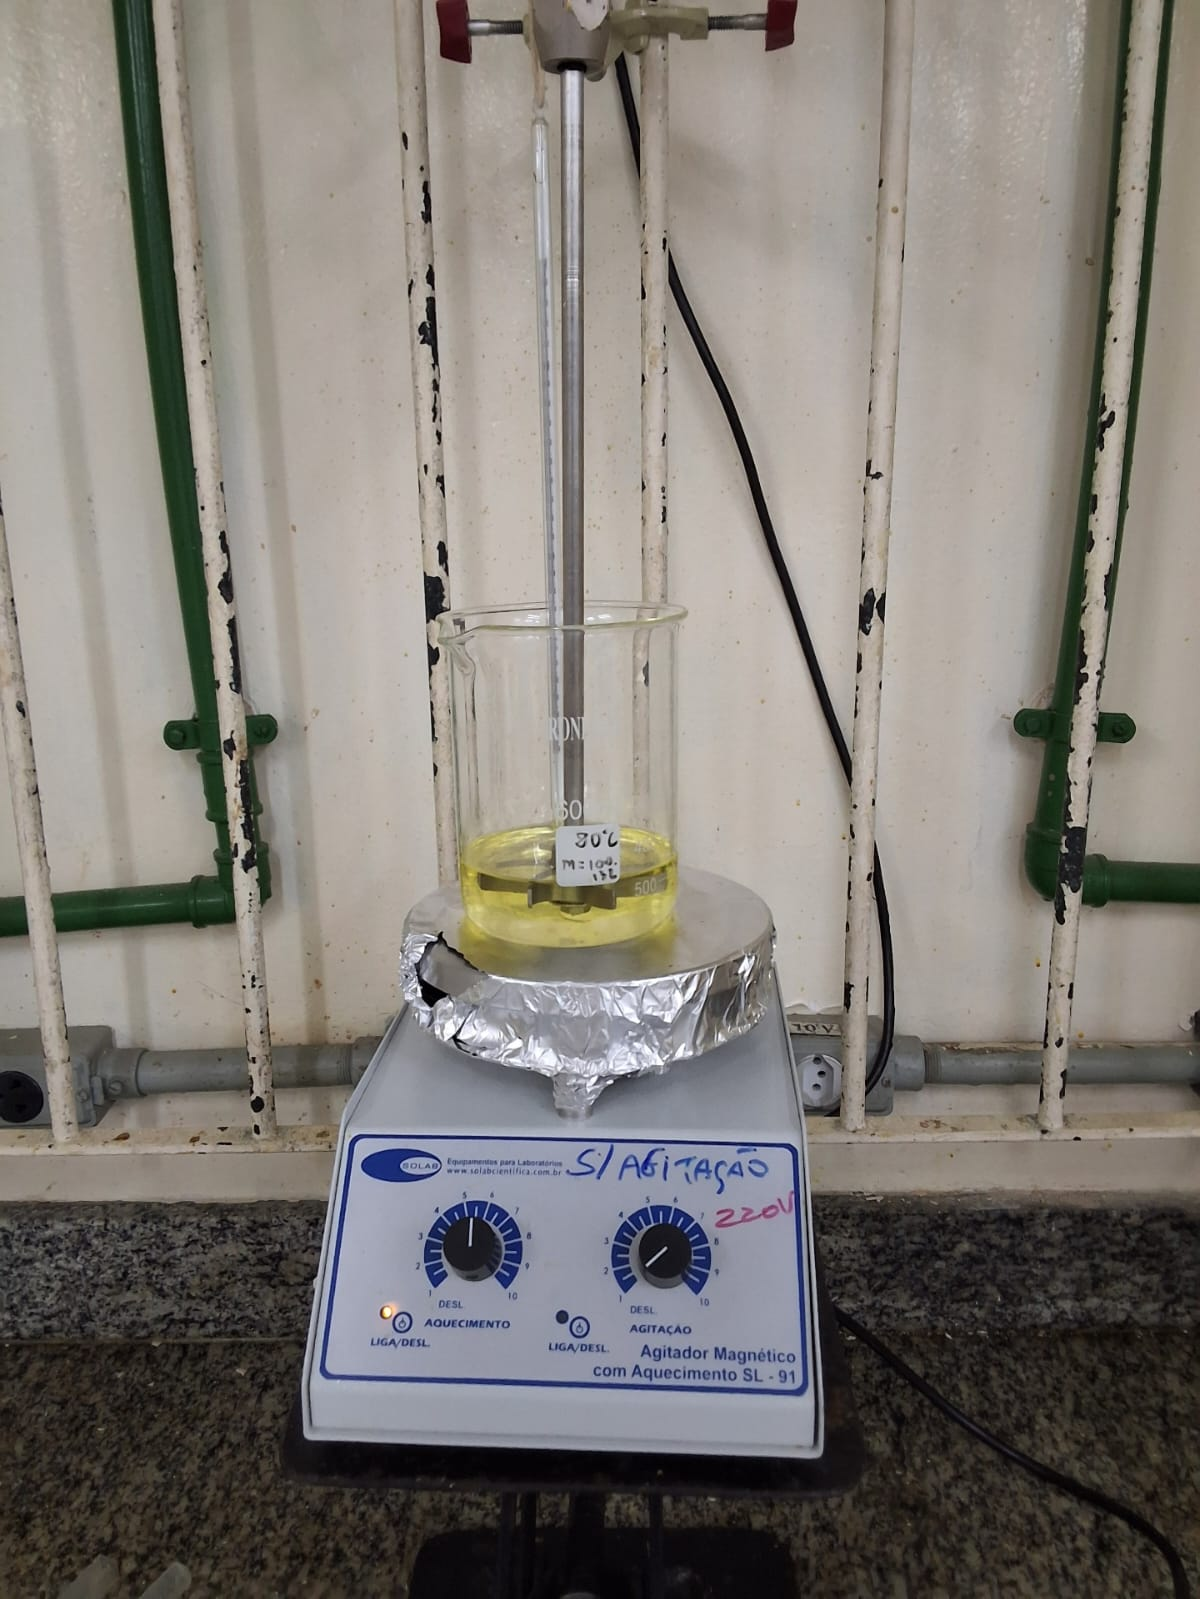
\includegraphics[width=0.4\textwidth]{src/fig/dia4/momento_0.jpg}
    \caption{Mistura do quarto dia logo após a adição da solução básica.}
    \label{fig:dia4_inicio}
\end{figure}

\begin{figure}[H]
    \centering
    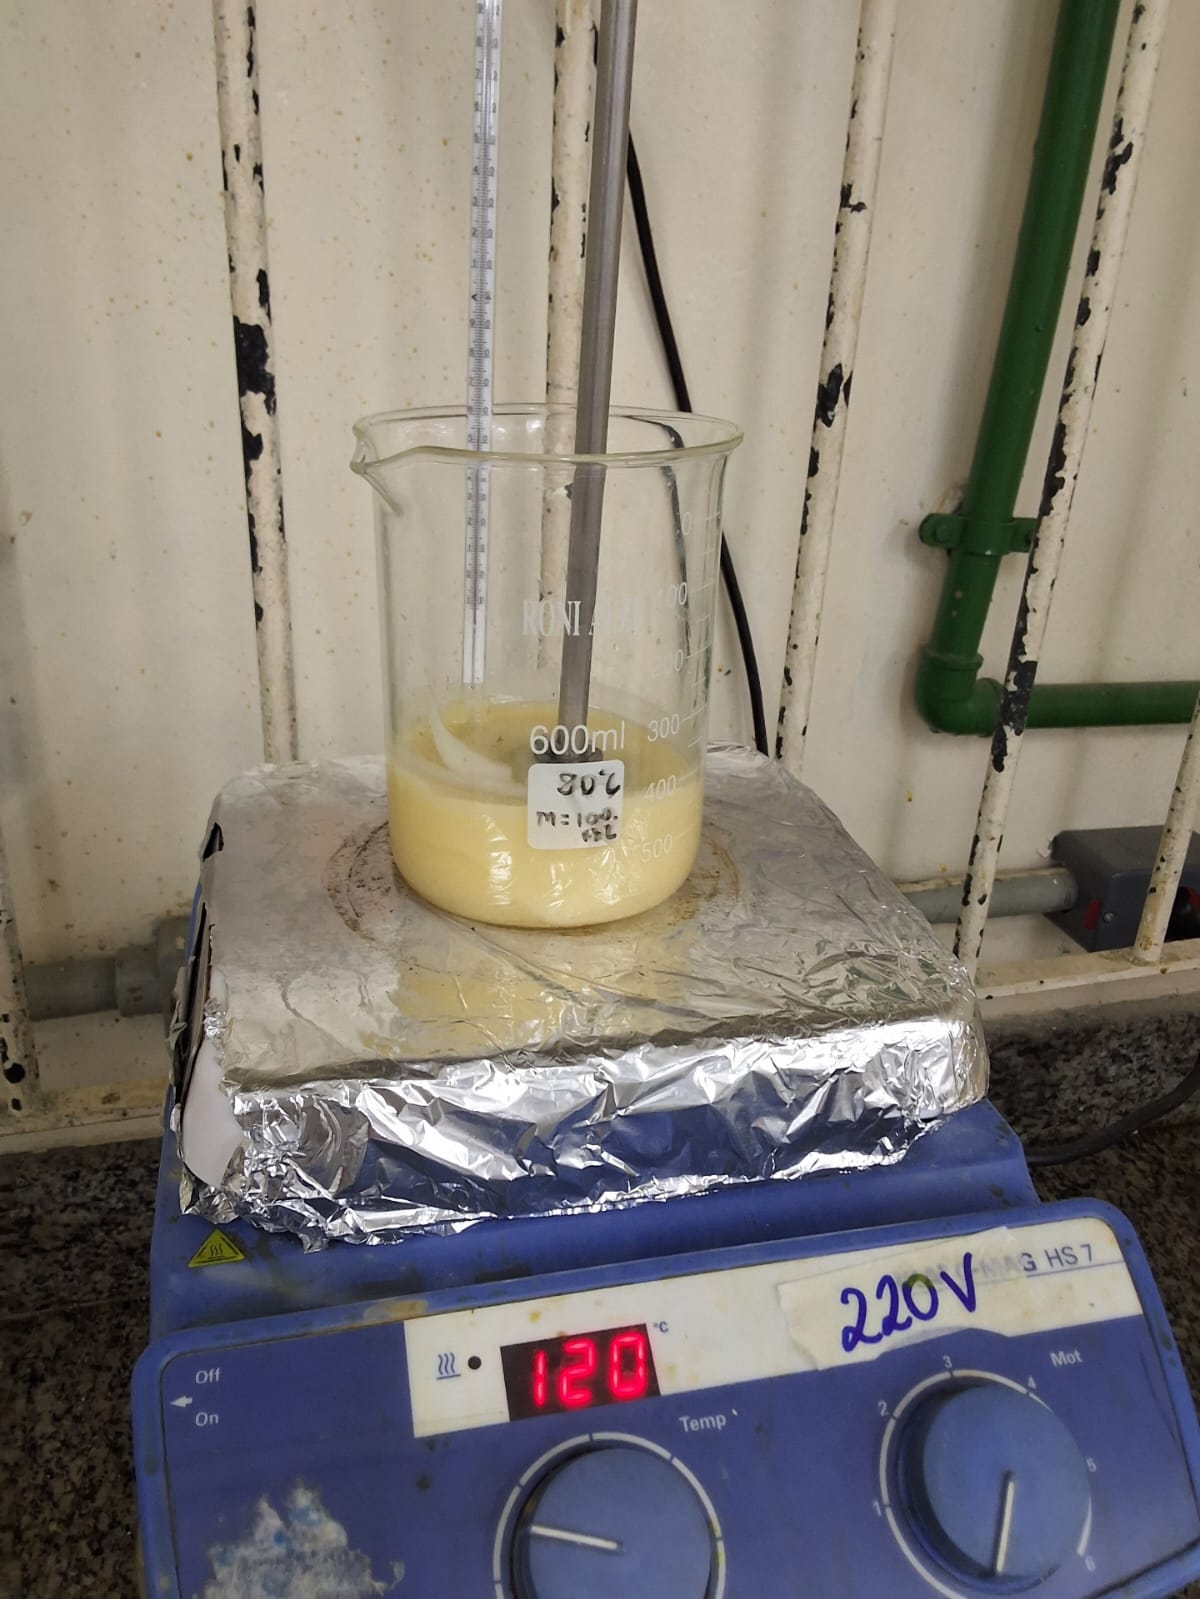
\includegraphics[width=0.4\textwidth]{src/fig/dia4/momento_2.jpg}
    \caption{Mistura do quarto dia próxima ao ponto de viscosidade ideal.}
    \label{fig:dia4_ponto}
\end{figure}

Em seguida, o material foi despejado nos moldes. Em razão do tempo perdido aguardando o resfriamento do óleo superaquecido, não foi possível registrar uma fotografia do produto final antes do início da cura.

\subsubsection{Quinto dia}

O quinto dia marcou a primeira utilização de etanol no experimento. O objetivo da prática era reduzir o pH final do produto, que havia mantido elevado nas amostras anteriores. Para isso, avaliaram-se duas alternativas: a adição de ácidos fracos (cítrico ou málico) ao final da reação ou a introdução de etanol como cossolvente, capaz de acelerar e homogeneizar a saponificação. Após discussão com o monitor e o professor, optou-se pelo uso do etanol.

Manteve-se a proporção de óleos da melhor reação obtida até então (terceiro dia), agora com a adição de etanol. A Tabela~\ref{tab:dia5_comparacao} apresenta os valores teóricos e os efetivamente realizados.

\begin{table}[H]
    \centering
    \footnotesize
    \caption{Composição teórica e realizada na amostra do quinto dia.}
    \label{tab:dia5_comparacao}
    \begin{tabular}{lcc} 
        \toprule
        \textbf{Parâmetro} & \textbf{Teórico} & \textbf{Efetuado} \\
        \midrule
        Massa de babaçu (g)        & 39,90  & 45,72  \\
        Massa de soja (g)          & 79,67  & 83,07  \\
        Massa total (g)            & 119,57 & 124,60 \\
        Perc. de babaçu (\%)       & 33,37  & 36,67  \\
        NaOH (g)                   & 18,48  & 19,18  \\
        Massa de ác. esteárico (g) & 3,58   & 4,05   \\
        \bottomrule
    \end{tabular}
\end{table}

Nesse dia, o óleo de babaçu encontrava-se sólido, sendo necessário liquefazê-lo em banho-maria antes do uso. Ao dissolver o ácido esteárico, a mistura de óleos apresentou leve turbidez, provavelmente em razão do estado físico inicial do babaçu. Em seguida, preparou-se a solução básica (Figura~\ref{fig:dia5_naoh}).

\begin{figure}[H]
    \centering
    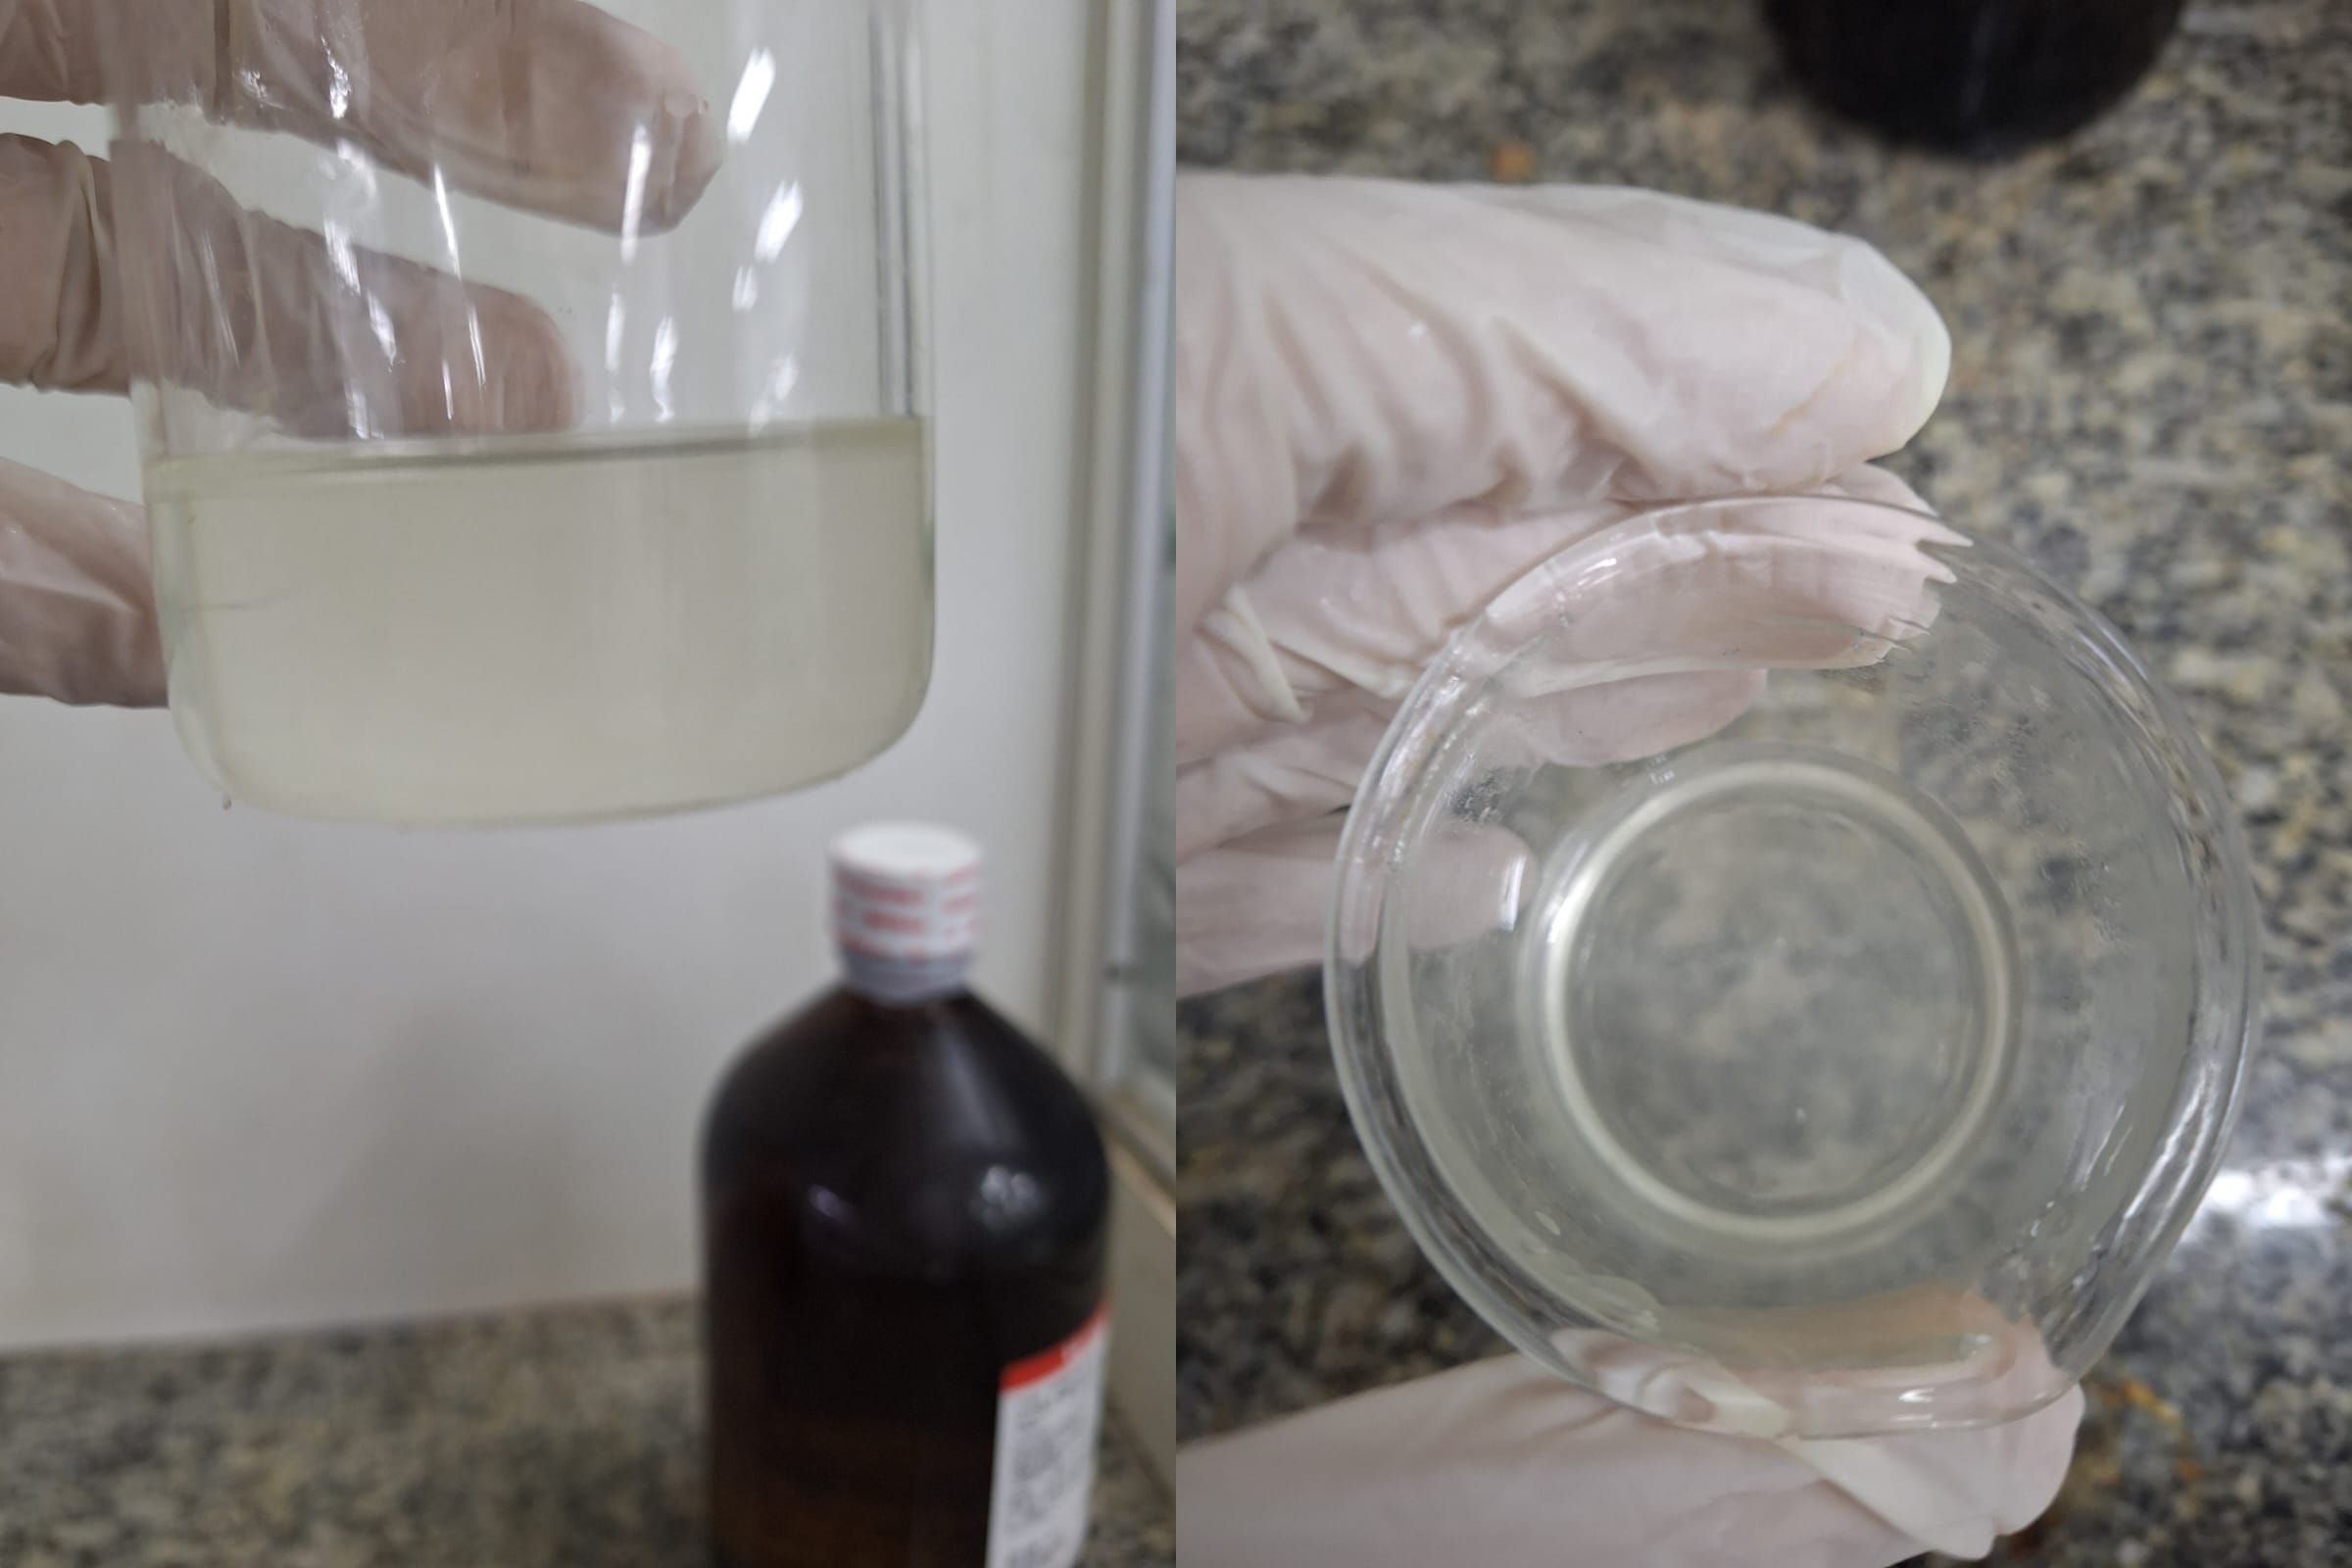
\includegraphics[width=0.8\textwidth]{src/fig/dia5/NaOH.jpg}
    \caption{Solução básica preparada no quinto dia.}
    \label{fig:dia5_naoh}
\end{figure}

O etanol disponível no laboratório possuía concentração de 95\%. Adotou-se uma fração de 10\% do volume de óleo, dentro da faixa prevista no procedimento (Seção~\ref{subsubsec:calc_alcool}). Aplicando a Equação~\ref{eq:alcool_isolado} para o volume de óleo dessa amostra (cerca de 138,8~ml), obtém-se $V_{95\%} = \frac{0,50}{0,95} \times 0,10 \times 138,8 \approx 7,30$~ml de etanol a 95\% (Figura~\ref{fig:dia5_alcool}).

\begin{figure}[H]
    \centering
    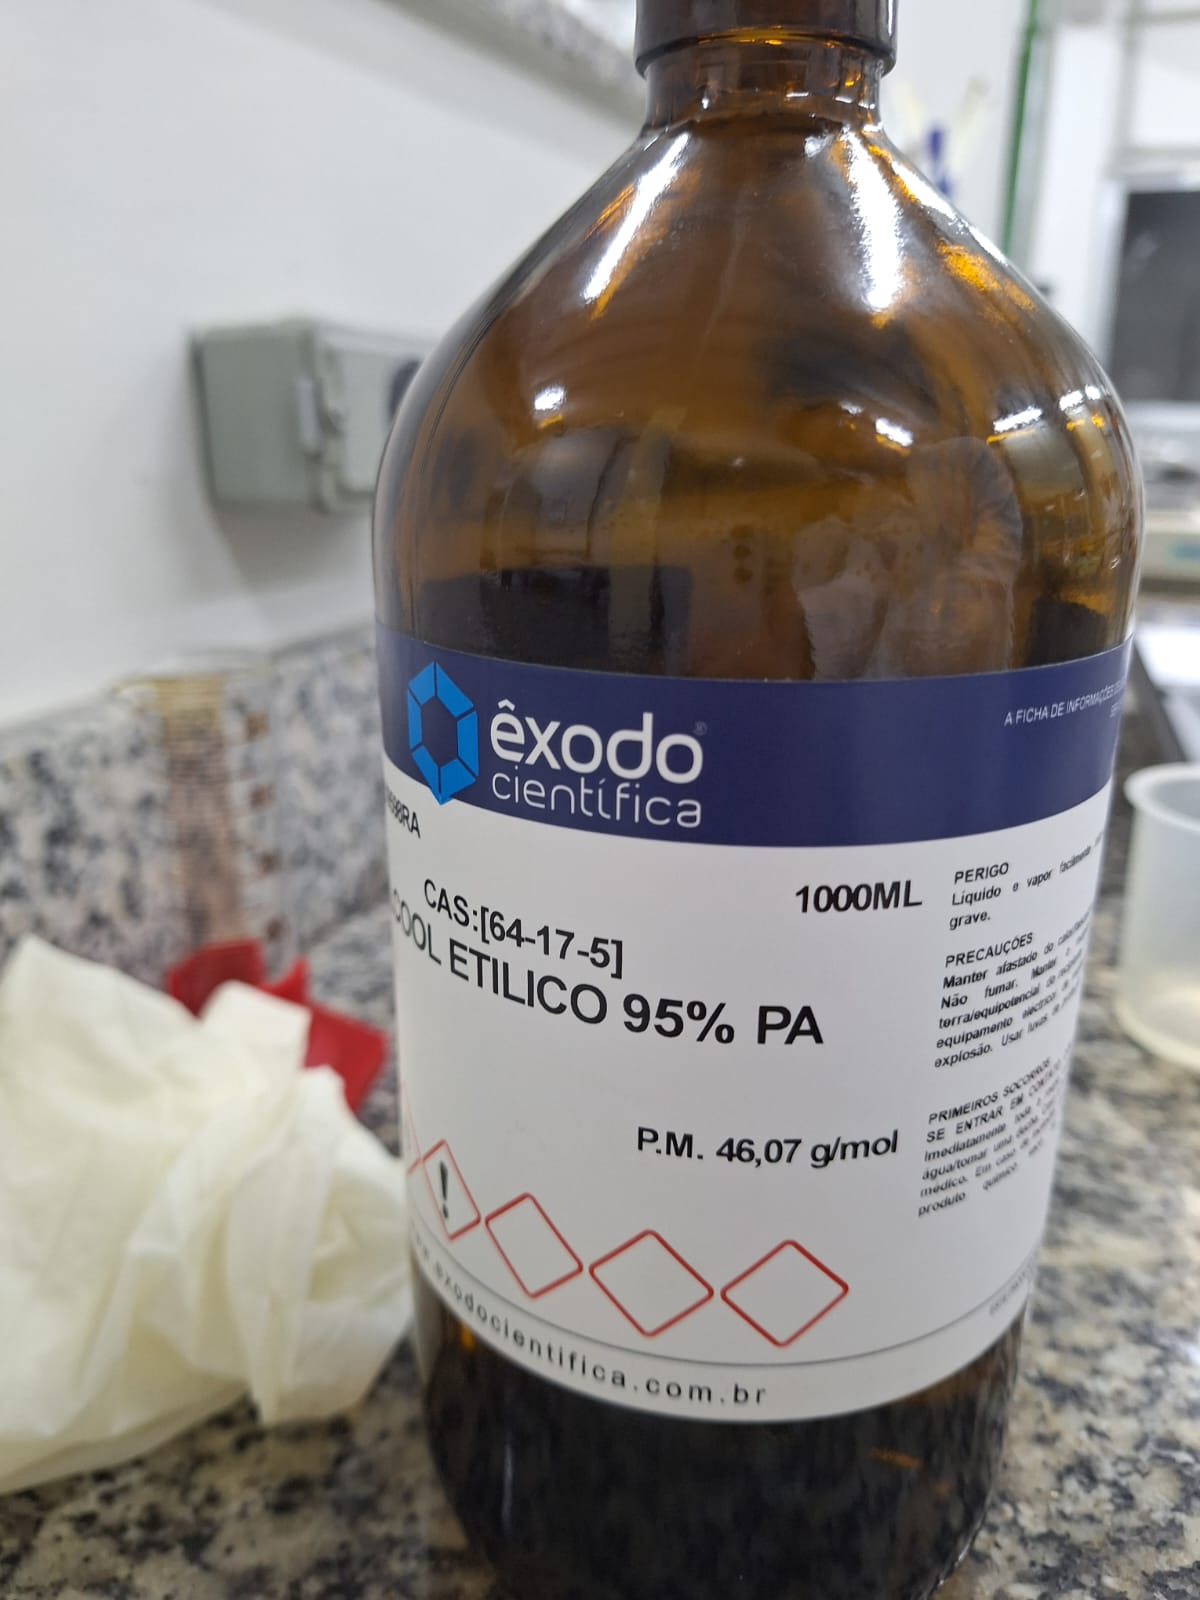
\includegraphics[width=0.3\textwidth]{src/fig/dia5/alcool.jpeg}
    \caption{Etanol utilizado no quinto dia.}
    \label{fig:dia5_alcool}
\end{figure}

Após a estabilização da mistura de óleos a 60~°C, adicionou-se o etanol e, em seguida, a solução básica. Um dos efeitos do álcool foi percebido imediatamente: a mistura tornou-se visivelmente mais clara (Figura~\ref{fig:dia5_claro}), indício de seu papel como cossolvente, ao reduzir a diferença de polaridade entre as fases oleosa e alcalina.

\begin{figure}[H]
    \centering
    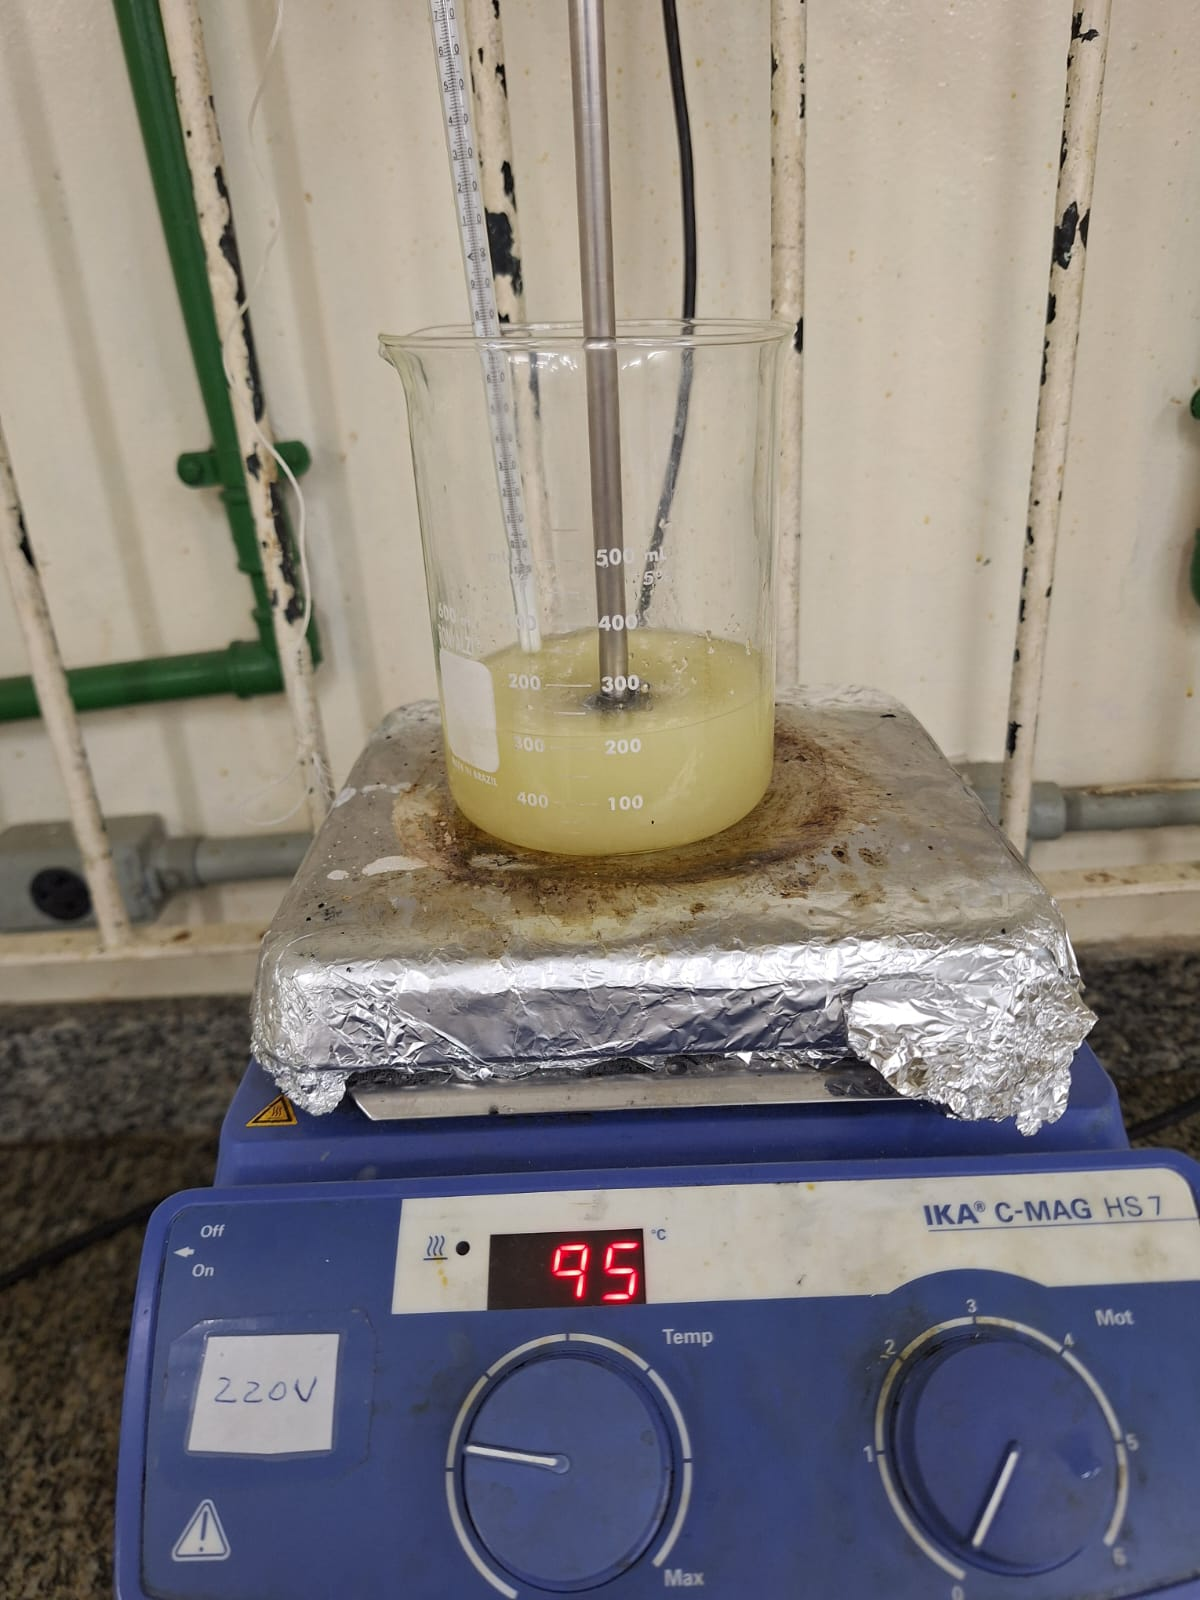
\includegraphics[width=0.4\textwidth]{src/fig/dia5/oleo_claro.jpeg}
    \caption{Mistura mais clara após a adição do etanol.}
    \label{fig:dia5_claro}
\end{figure}

A partir daí, seguiu-se o procedimento padrão, ajustando-se a potência do agitador conforme o aumento da viscosidade. A agitação iniciou-se no nível 1; aos 2 minutos, passou para 1,5; aos 4 minutos, a viscosidade aumentou tanto que o agitador travou, sendo necessário segurar o becker no lugar para que o agitador continuasse a girar, com a potência elevada para 2 (Figura~\ref{fig:dia5_becker}); aos 8 minutos, passou para 2,5, quando a reação foi interrompida, por já ter atingido o ponto de "purê de batatas".

\begin{figure}[H]
    \centering
    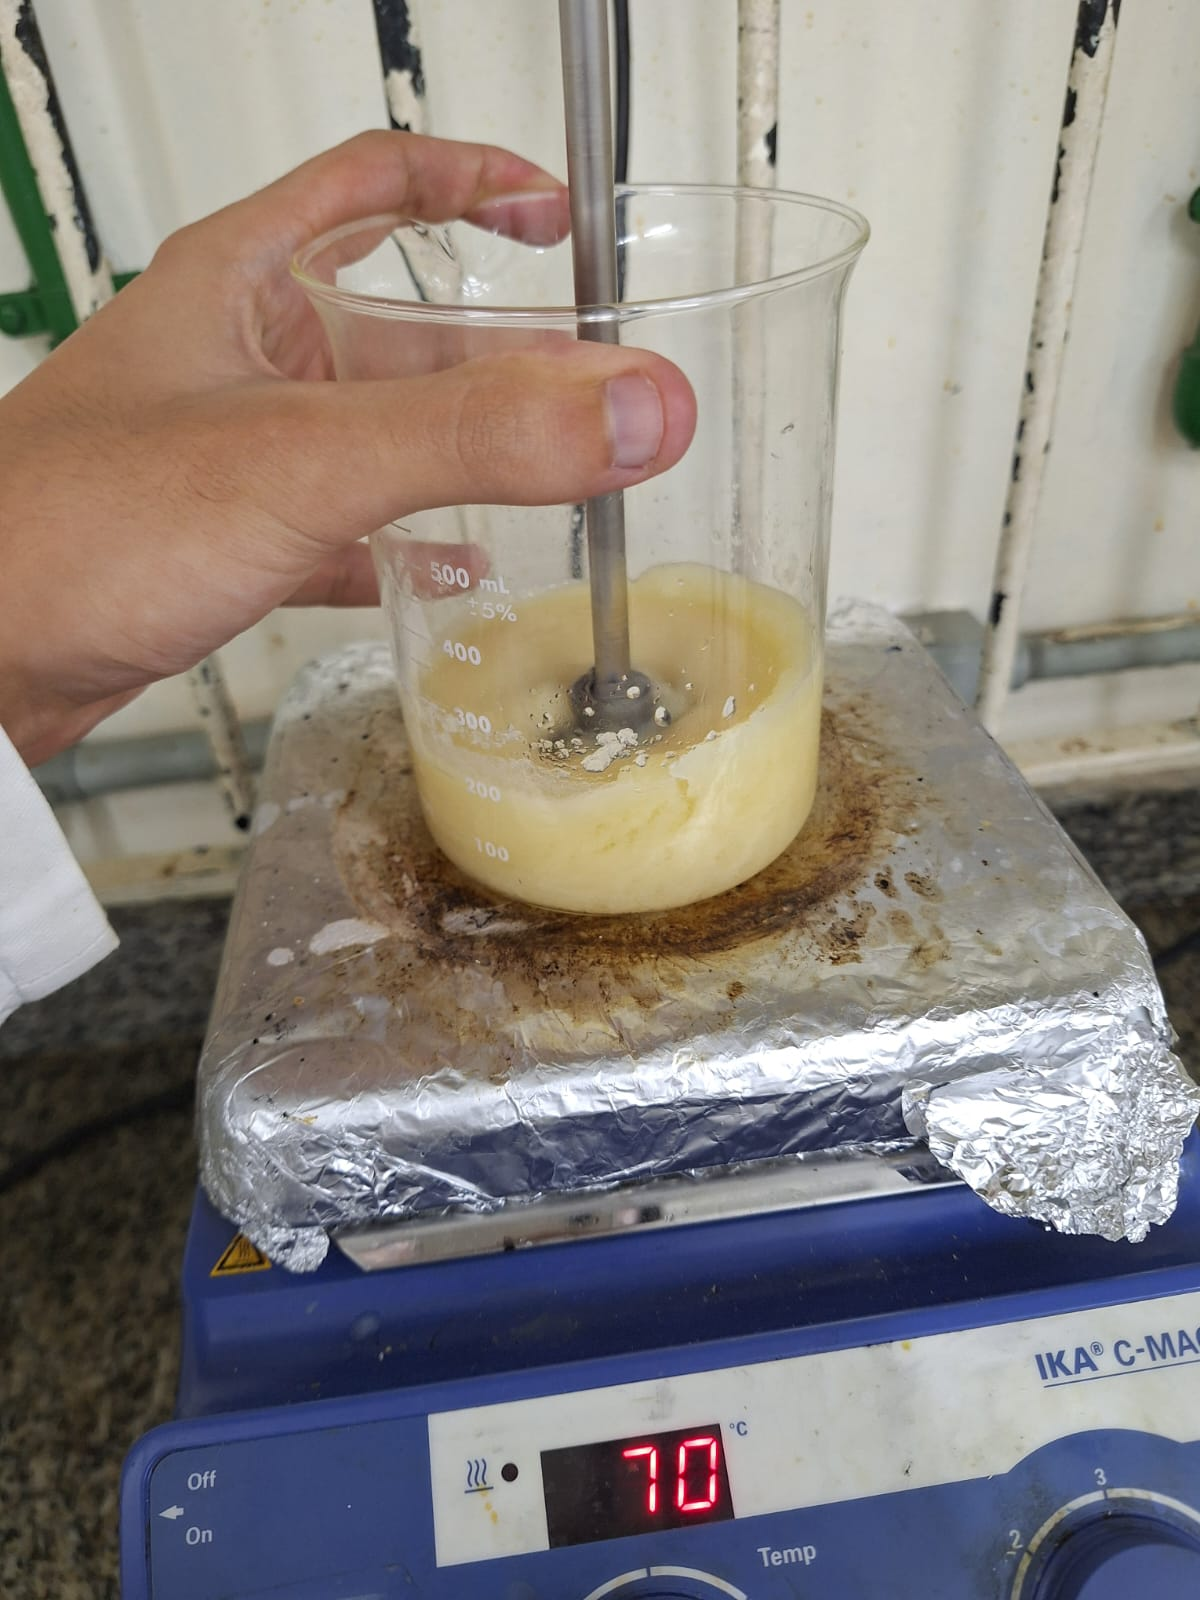
\includegraphics[width=0.3\textwidth]{src/fig/dia5/segurando_becker.jpeg}
    \caption{Becker sendo mantido no lugar para permitir a agitação da mistura, já bastante viscosa.}
    \label{fig:dia5_becker}
\end{figure}

O pH final medido ao término da etapa de bancada foi de 10 — o menor valor obtido até então, o que corrobora a hipótese de que o etanol, ao acelerar e homogeneizar a saponificação, favorece um maior consumo da base dentro do tempo de reação. Não foi possível registrar uma fotografia do produto final.

\paragraph{Avaliação após a cura.} A amostra do quinto dia, primeira produzida com etanol, é apresentada após o período de cura na Figura~\ref{fig:dia5_curado}. Sem dúvidas em questão de aparência, textura e coloração essa é a mostra mais bem contraída que foi feita. Além disso por algum motivo o uso do álcool deixou o cheiro do sabão formado muito mais agradável.

\begin{figure}[H]
    \centering
    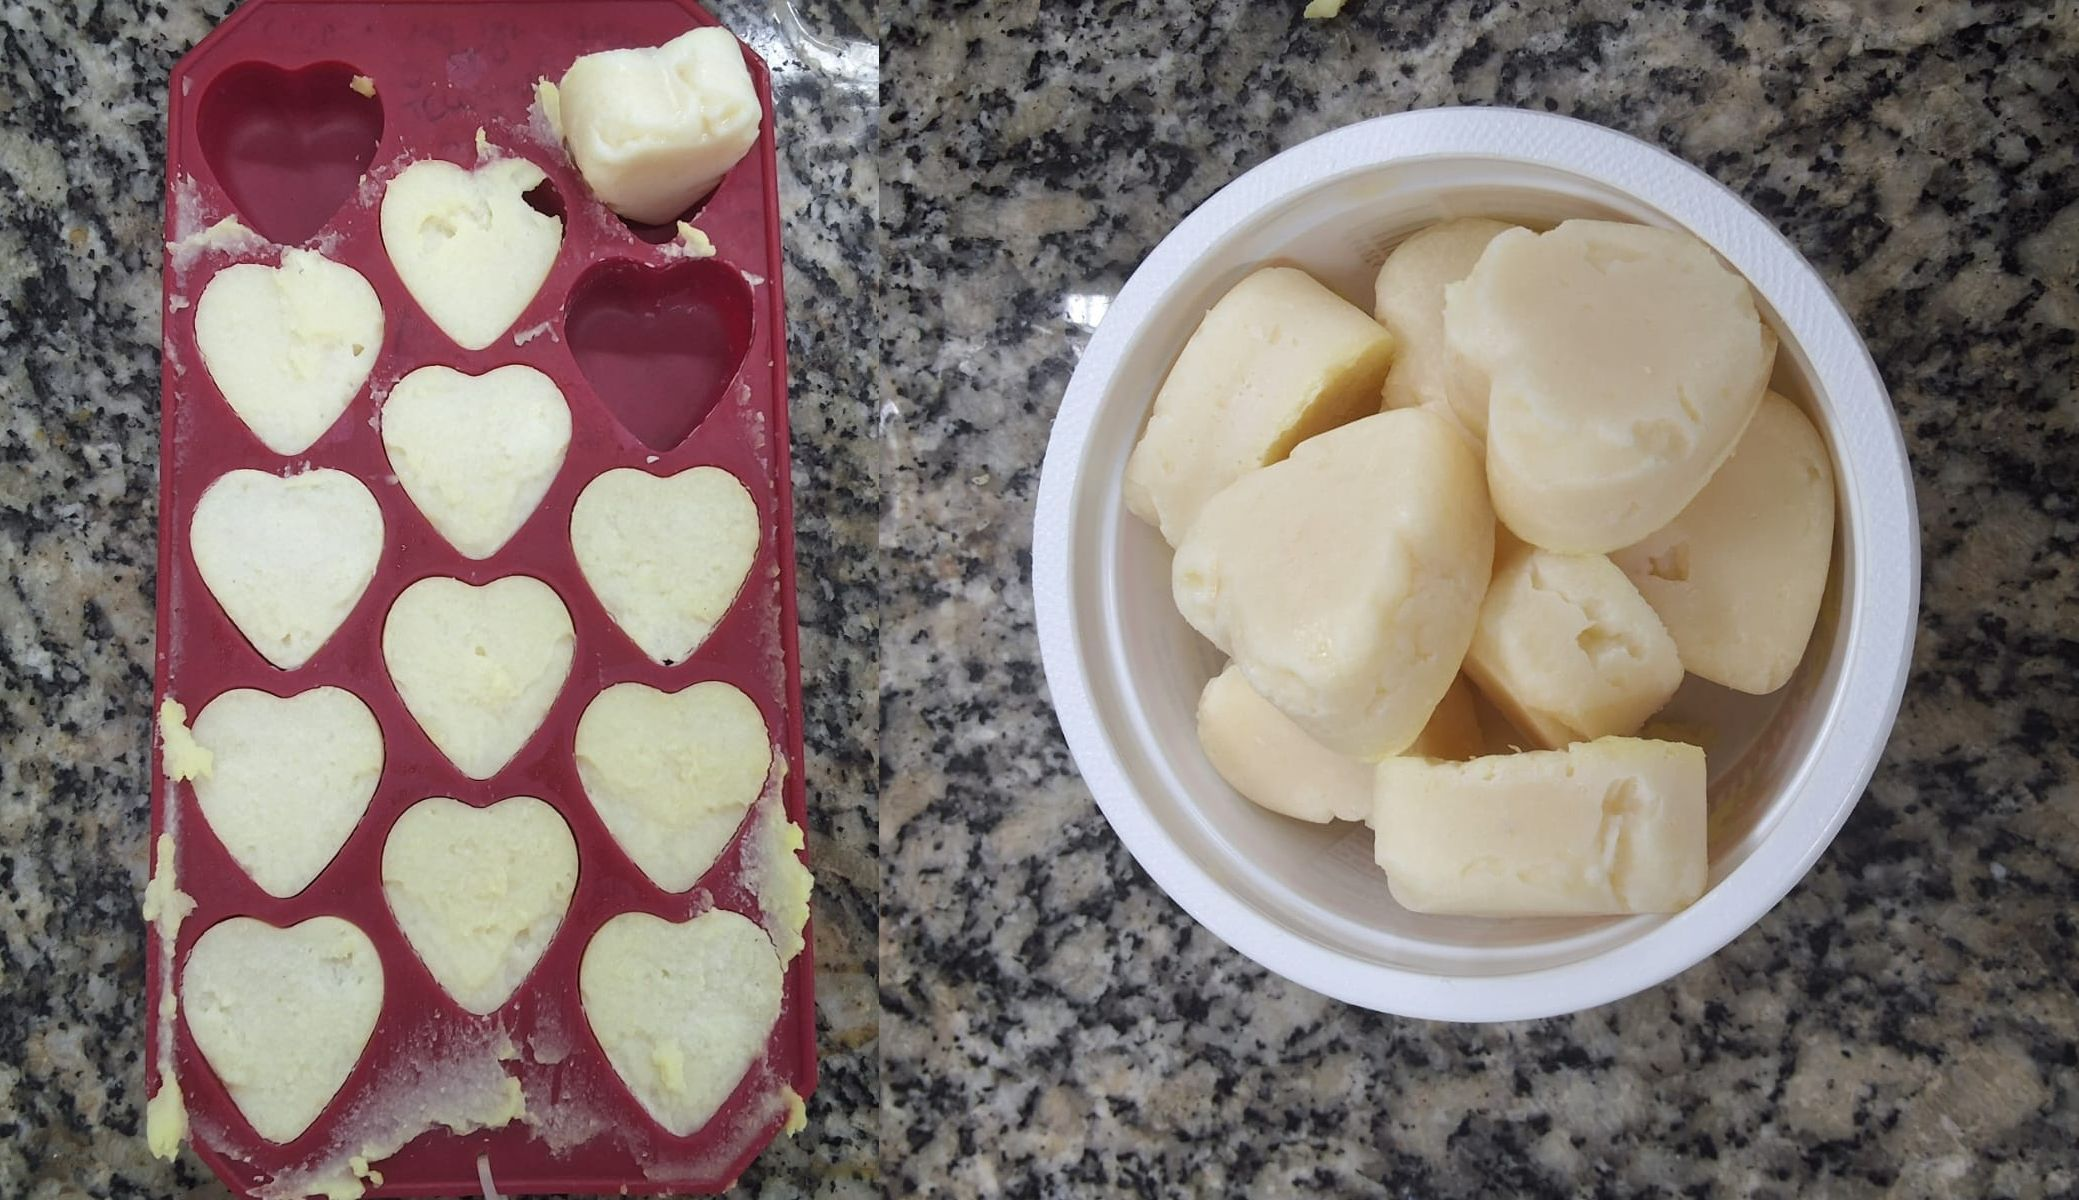
\includegraphics[width=0.8\textwidth]{src/fig/dia5/resultado.jpg}
    \caption{Amostra do quinto dia após a cura.}
    \label{fig:dia5_curado}
\end{figure}

\subsubsection{Sexto dia}

O sexto dia repetiu o experimento do quinto, reduzindo-se a quantidade de etanol. No dia anterior, a reação foi tão rápida que o ponto ideal foi atingido antes dos 15 minutos; por isso, a fração de etanol foi reduzida de 10\% para 7\% do volume de óleo. Manteve-se a proporção de óleos de referência (cerca de 33\% de babaçu). A Tabela~\ref{tab:dia6_comparacao} apresenta os valores teóricos e os efetivamente realizados.

\begin{table}[H]
    \centering
    \footnotesize
    \caption{Composição teórica e realizada na amostra do sexto dia.}
    \label{tab:dia6_comparacao}
    \begin{tabular}{lcc}
        \toprule
        \textbf{Parâmetro} & \textbf{Teórico} & \textbf{Efetuado} \\
        \midrule
        Massa de babaçu (g)        & 39,90  & 40,14  \\
        Massa de soja (g)          & 79,67  & 81,52  \\
        Massa total (g)            & 119,57 & 121,66 \\
        Perc. de babaçu (\%)       & 33,37  & 32,99  \\
        NaOH (g)                   & 18,48  & 18,51  \\
        Massa de ác. esteárico (g) & 3,58   & 3,59   \\
        \bottomrule
    \end{tabular}
\end{table}

Como no quinto dia, o óleo de babaçu encontrava-se sólido, sendo necessário liquefazê-lo em banho-maria; ao dissolver o ácido esteárico, a mistura novamente apresentou leve turbidez. A preparação da solução básica, porém, enfrentou um problema: na primeira tentativa, a solução ficou com diversos corpos flutuantes (Figura~\ref{fig:dia6_naoh_ruim}), provavelmente porque a soda cáustica estava no fim e, junto às lentilhas (formato do sólido), havia certa quantidade de impurezas semelhantes a areia. Por esse motivo, a solução foi descartada e preparada novamente, com seleção mais cuidadosa das lentilhas; ainda assim, a solução final manteve alguns corpos flutuantes (Figura~\ref{fig:dia6_naoh}).

\begin{figure}[H]
    \centering
    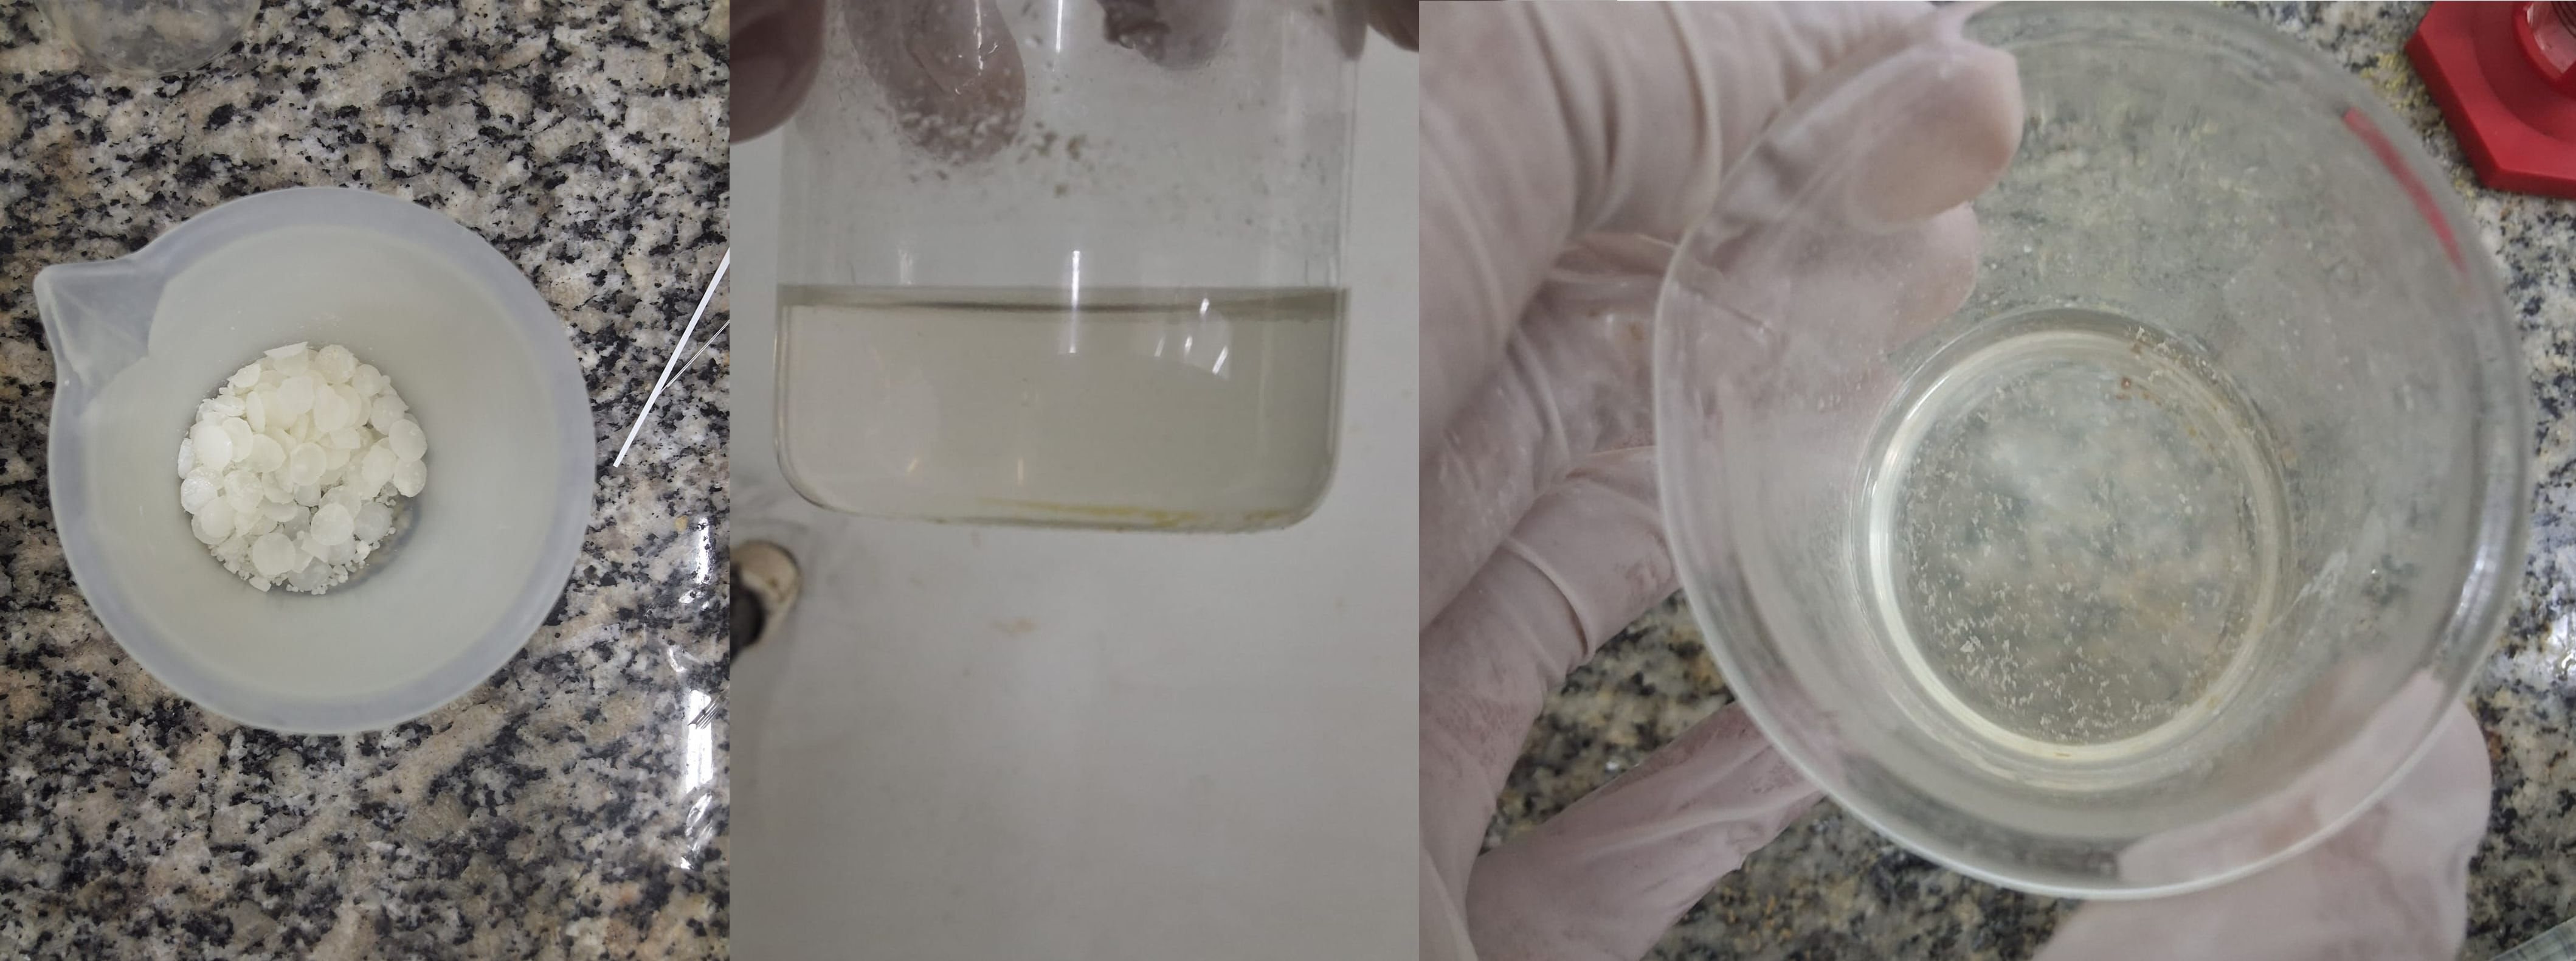
\includegraphics[width=0.9\textwidth]{src/fig/dia6/ruim_NaOH.jpg}
    \caption{Primeira solução básica do sexto dia, descartada por conter corpos flutuantes.}
    \label{fig:dia6_naoh_ruim}
\end{figure}

\begin{figure}[H]
    \centering
    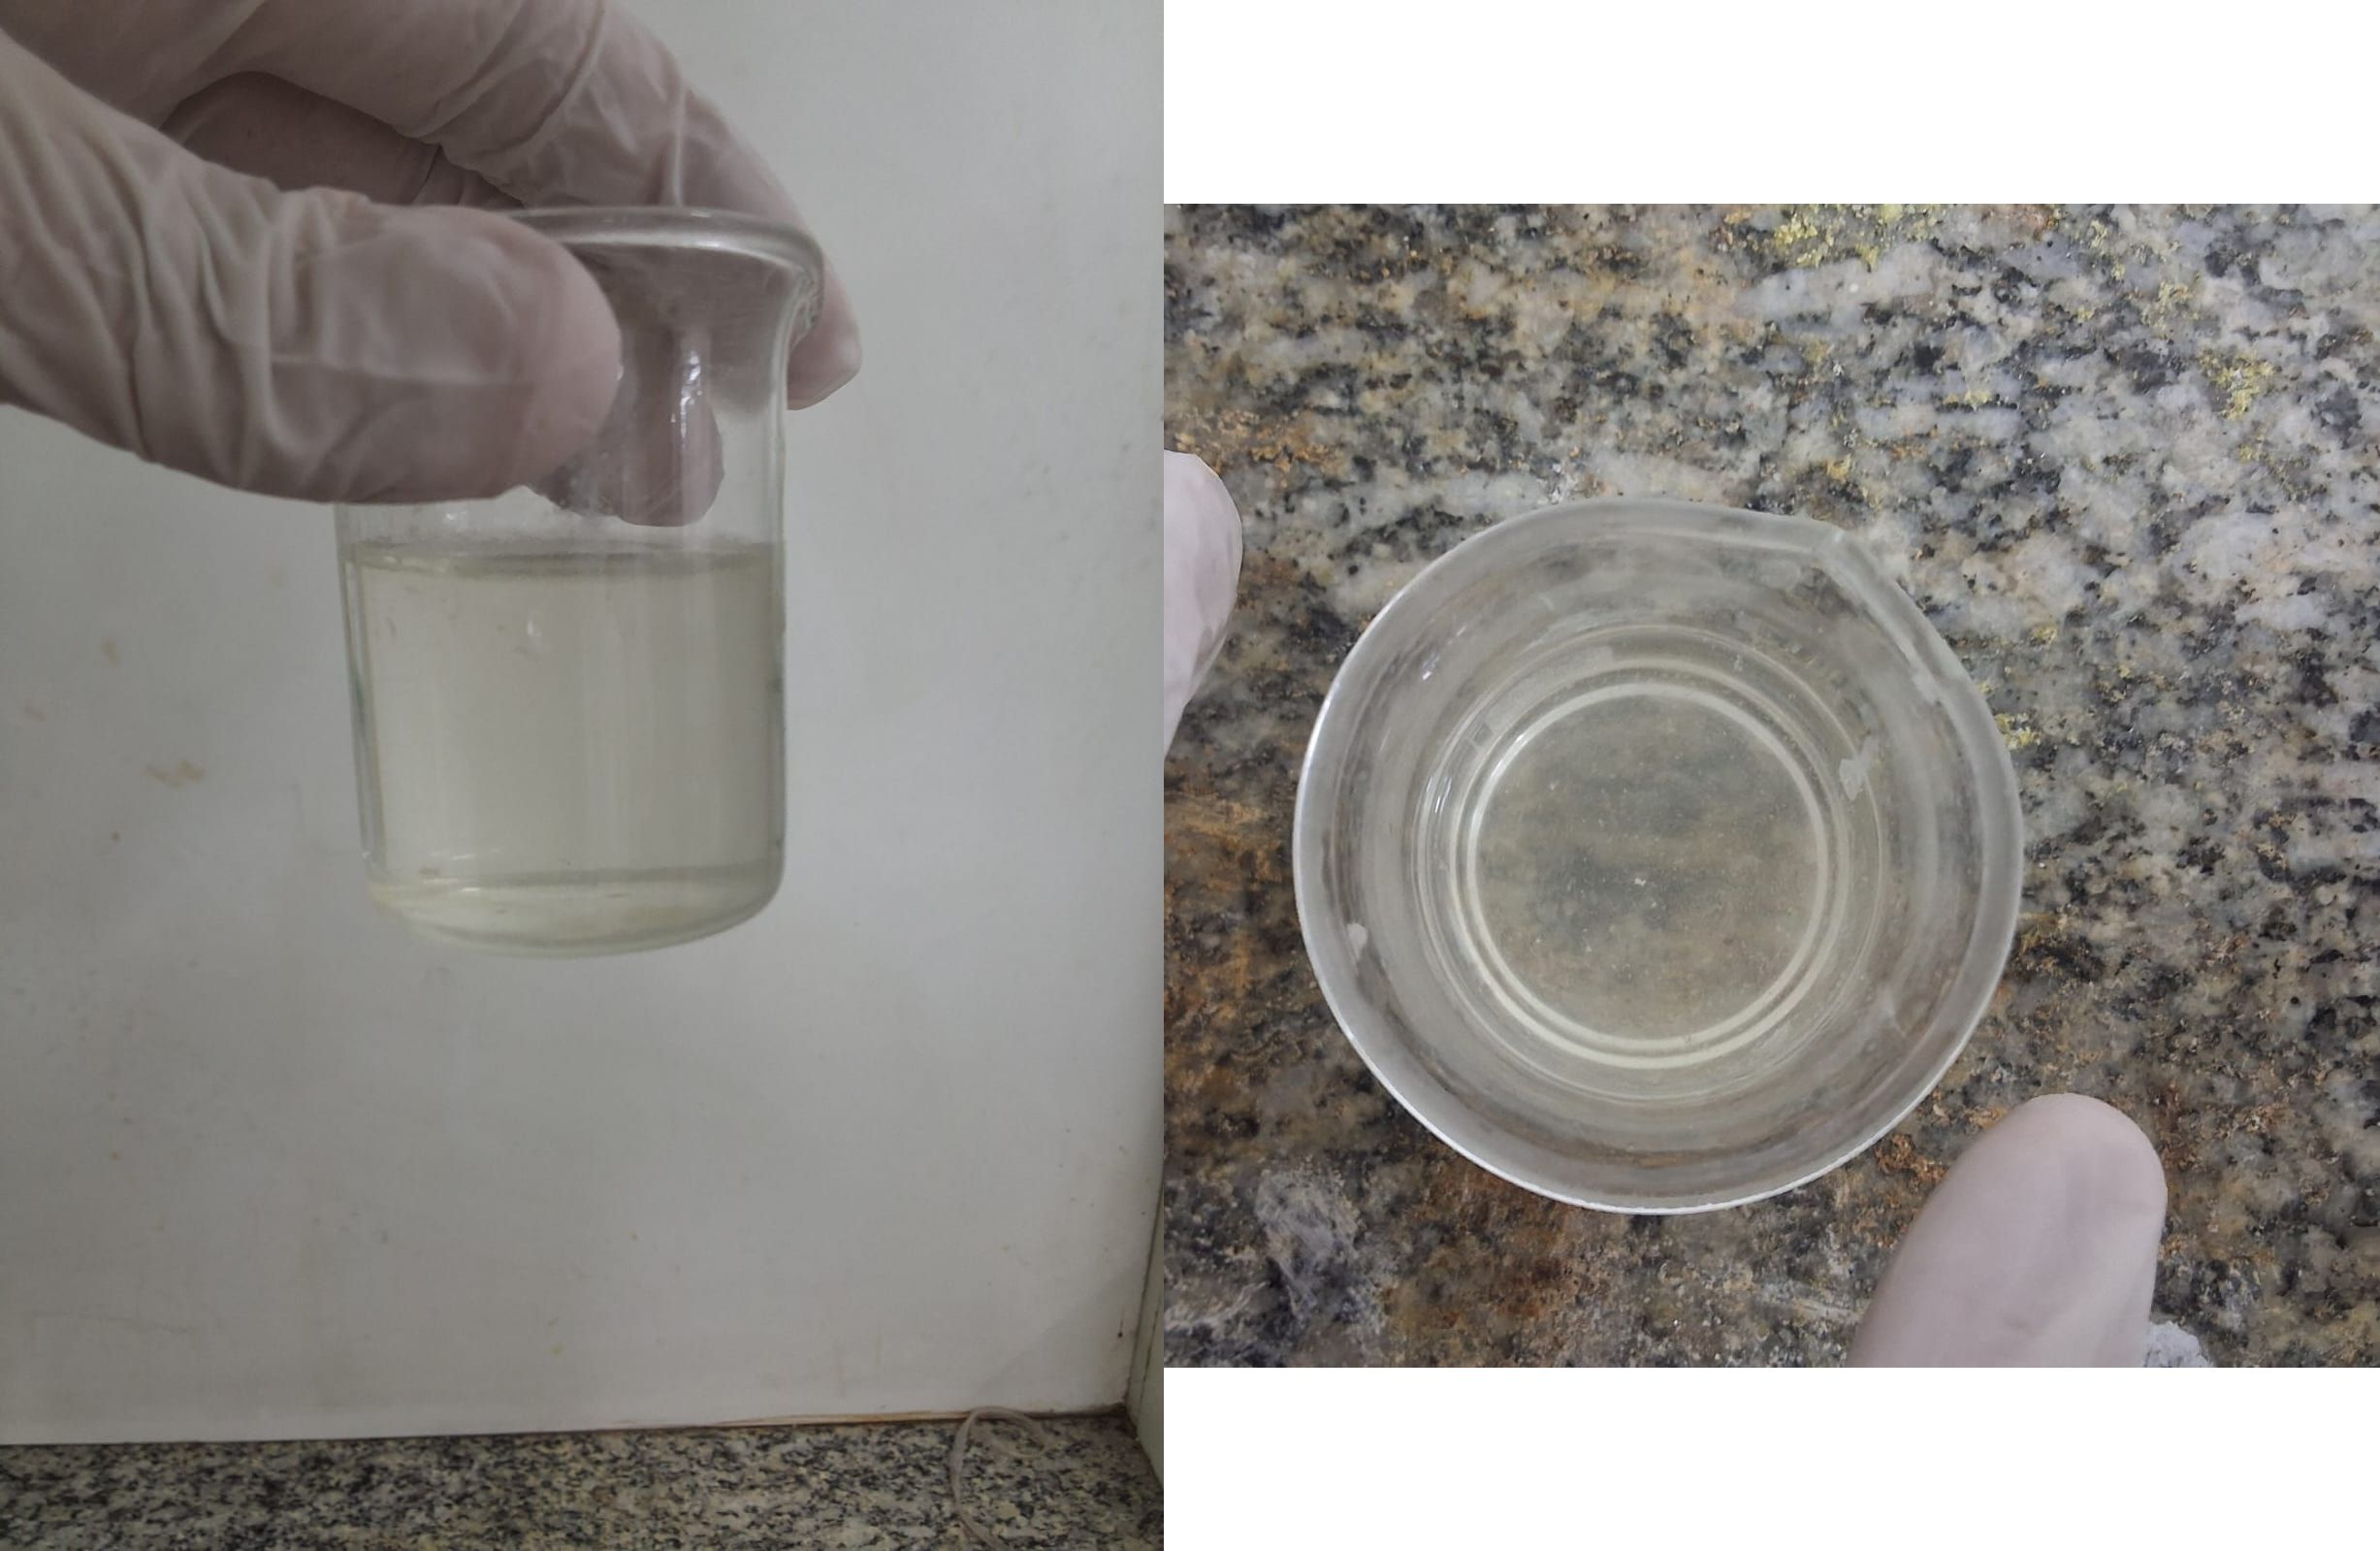
\includegraphics[width=0.7\textwidth]{src/fig/dia6/NaOH.jpg}
    \caption{Solução básica do sexto dia, preparada pela segunda vez.}
    \label{fig:dia6_naoh}
\end{figure}

Adotando a fração de 7\% do volume de óleo, para o cálculo de quantidade de etanol e aplicando a Equação~\ref{eq:alcool_isolado} para o volume de óleo dessa amostra (cerca de 132,33~ml), obtém-se $V_{95\%} = \frac{0,50}{0,95} \times 0,07 \times 132,33 \approx 4,87$~ml.

Após a estabilização da mistura de óleos a 60~°C, adicionaram-se o etanol e, em seguida, a solução básica; novamente, a mistura tornou-se visivelmente mais clara. Seguiu-se o procedimento padrão, com ajuste da potência do agitador conforme o aumento da viscosidade: a agitação iniciou-se no nível 1; aos 2 minutos, passou para 1,5; e, aos 5 minutos, com o aumento acentuado da viscosidade, elevou-se para 2, passando-se a segurar o becker para evitar o problema enfrentado no dia anterior (Figura~\ref{fig:dia6_becker}). Aos 8 minutos, a reação foi interrompida, por já ter atingido o ponto de "purê de batatas".

\begin{figure}[H]
    \centering
    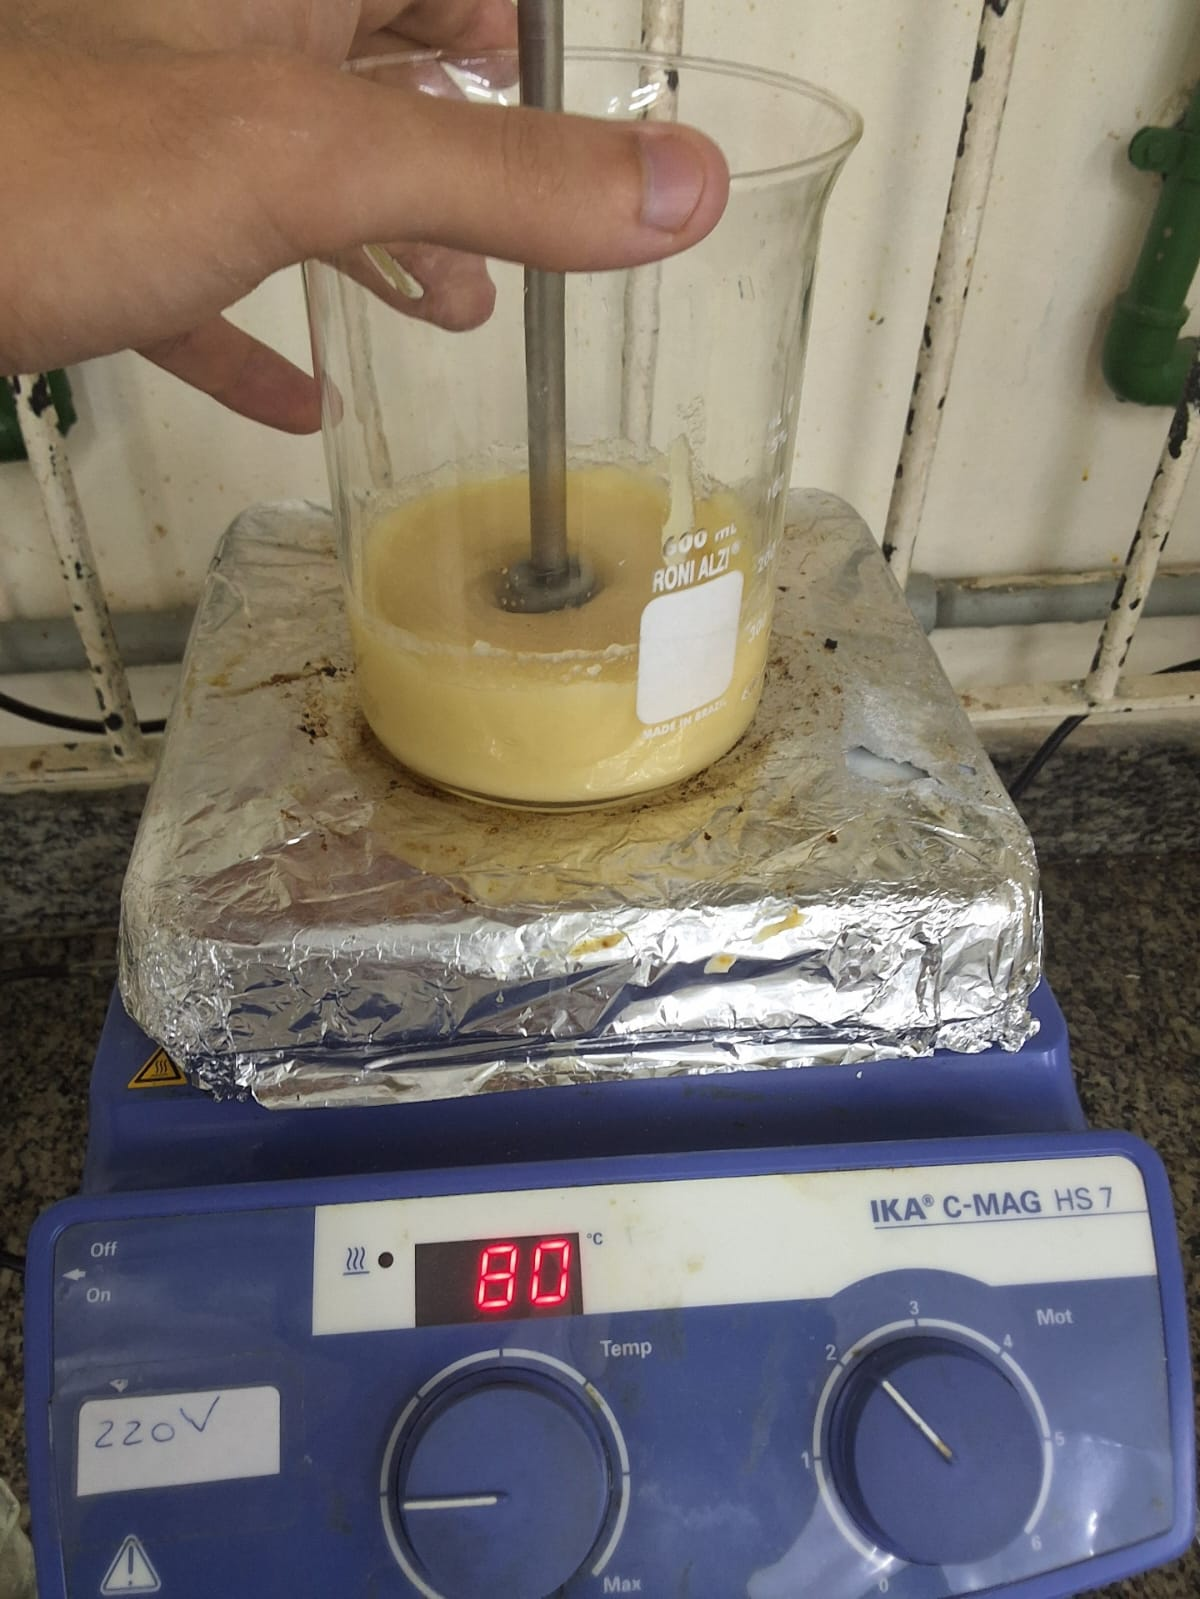
\includegraphics[width=0.3\textwidth]{src/fig/dia6/segurando_becker.jpeg}
    \caption{Becker sendo mantido no lugar durante a agitação da mistura.}
    \label{fig:dia6_becker}
\end{figure}

O pH final medido ao término da etapa de bancada foi de 10,5 — discretamente superior ao do quinto dia (10), o que é coerente com a menor quantidade de etanol empregada. O produto obtido é apresentado na Figura~\ref{fig:dia6_final}.

\begin{figure}[H]
    \centering
    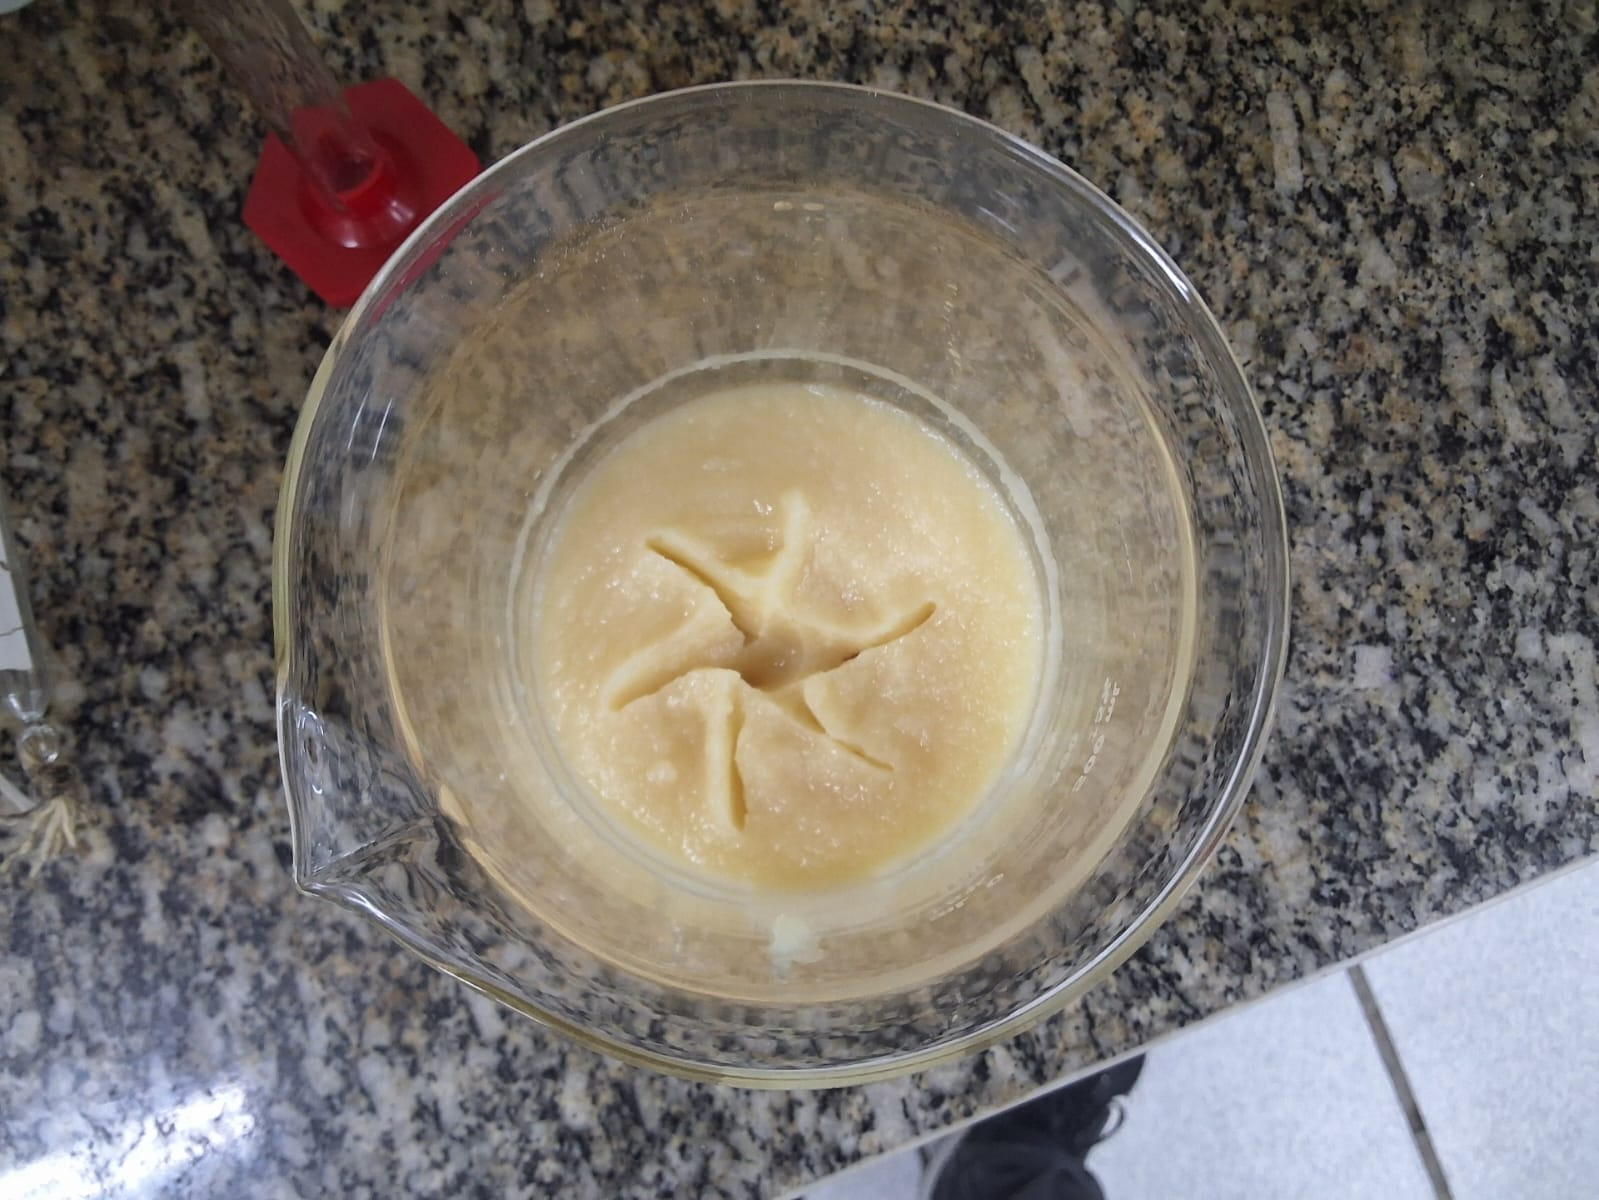
\includegraphics[width=0.4\textwidth]{src/fig/dia6/final.jpeg}
    \caption{Produto final do sexto dia.}
    \label{fig:dia6_final}
\end{figure}

\subsubsection{Sétimo dia}

A última aula foi dedicada à caracterização de todos os produtos obtidos ao longo das seis práticas anteriores. Como exceção, a amostra~2 do primeiro dia foi excluída da caracterização, por ter resultado em um produto de qualidade muito ruim, conforme discutido anteriormente.

\paragraph{Densidade, formação de bolhas e solubilidade.} Para cada produto, coletou-se uma amostra de aproximadamente 2,5~g, colocada em uma proveta. O nível da proveta foi registrado em três momentos: antes da adição da amostra ($N_i = 50$~ml), imediatamente após a adição ($N_0$) e dez minutos depois ($N_{10}$). A densidade do sabão foi calculada pela Equação~\ref{eq:densidade}.

\begin{equation}
    \text{densidade} = \frac{m}{N_0 - N_i}
    \label{eq:densidade}
\end{equation}

\noindent em que $m$ é a massa da amostra. O valor de $N_{10}$ foi utilizado para comparar a solubilidade entre os sabões. Além disso, durante o primeiro minuto de espera para a leitura de $N_{10}$, a proveta foi agitada vigorosamente para gerar bolhas e avaliar a sua qualidade. Os resultados estão reunidos na Tabela~\ref{tab:dia7_caracterizacao}.

\begin{table}[H]
    \centering
    \footnotesize
    \caption{Caracterização de densidade e solubilidade dos sabões produzidos.}
    \label{tab:dia7_caracterizacao}
    \begin{tabular}{ccccc}
        \toprule
        \textbf{Amostra} & \textbf{Massa (g)} & \textbf{$N_0$ (ml)} & \textbf{$N_{10}$ (ml)} & \textbf{Densidade (g/ml)} \\
        \midrule
        Dia 1 & 2,49 & 52,5 & 52,0 & 0,996 \\
        Dia 2 & 2,48 & 52,5 & 51,5 & 0,992 \\
        Dia 3 & 2,49 & 52,0 & 52,0 & 1,245 \\
        Dia 4 & 2,49 & 52,0 & 52,0 & 1,245 \\
        Dia 5 & 2,54 & 52,5 & 52,5 & 1,016 \\
        Dia 6 & 2,51 & 52,5 & 52,0 & 1,004 \\
        \bottomrule
    \end{tabular}
\end{table}

Em todas as amostras, o teste de bolhas apresentou formação abundante de espuma, que se manteve estável após os dez minutos de espera (Figura~\ref{fig:dia7_bolhas}). Quanto à densidade, os sabões dos dias 3 e 4 — produzidos com ácido esteárico e sem etanol — apresentaram os maiores valores (cerca de 1,25~g/ml), enquanto os demais ficaram próximos de 1,0~g/ml. Vale ressaltar, contudo, que a precisão do método é limitada: o deslocamento medido foi de apenas 2,0 a 2,5~ml, lido em uma proveta com resolução de 2,0~ml, de modo que pequenas variações de leitura afetam significativamente o valor calculado.

\begin{figure}[H]
    \centering
    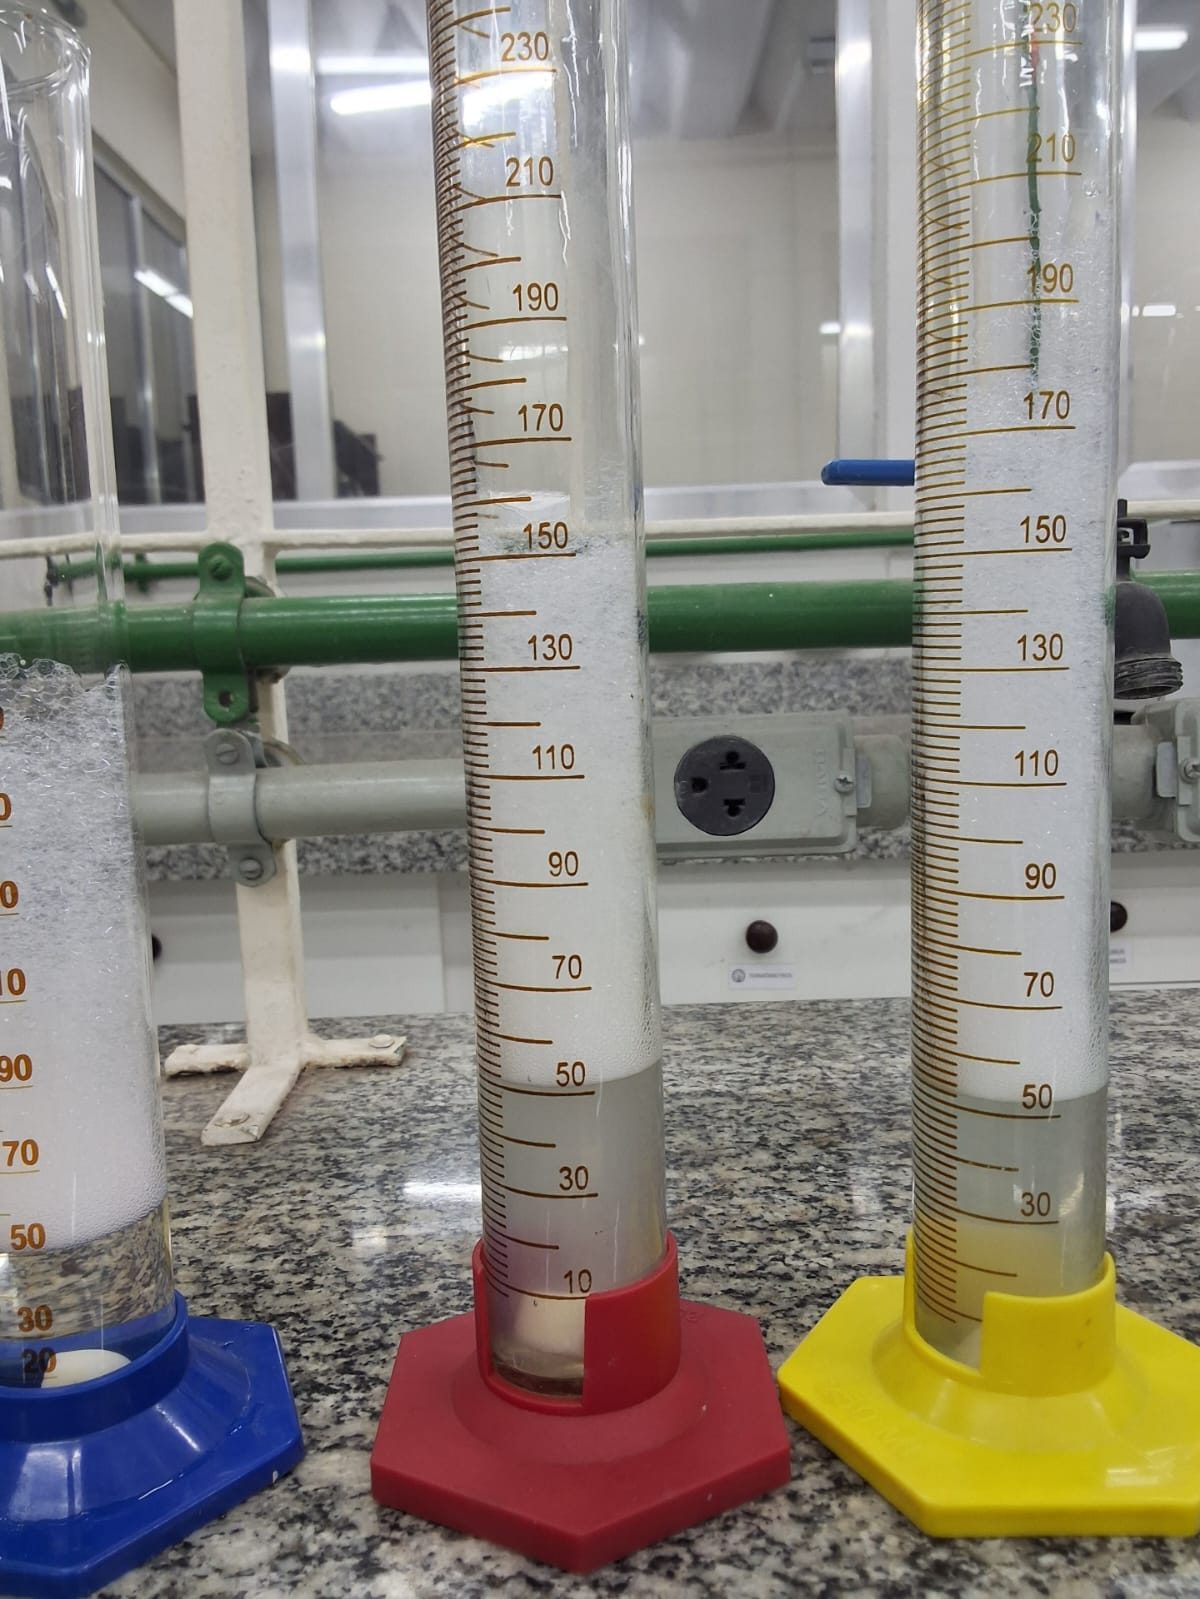
\includegraphics[width=0.4\textwidth]{src/fig/dia7/d5_bolha_10.jpeg}
    \caption{Teste de formação de bolhas, representativo das amostras caracterizadas.}
    \label{fig:dia7_bolhas}
\end{figure}

\paragraph{Teste de pH.} As provetas foram mantidas com as amostras por 35 minutos, de modo a dissolver uma quantidade significativa de sabão na água. Em seguida, os 50~ml de água, já sem a barra de sabão, foram transferidos para um becker. Dessa forma a região sensível de um papel de tornassol (papel indicador de pH) foi submersa por 1 a 2 segundos na água com sabão dissolvido, realizando-se então a leitura, de forma geral todos resultaram no mesmo valor 9 de pH.

\subsubsection{Último experimento}

Após o término da última aula, foi realizado em casa um experimento complementar de limpeza, com o objetivo de comparar a capacidade dos produtos de dissolver gordura em água. Para isso, foram utilizadas pequenas amostras dos sabões das aulas 1, 4, 5 e 6 — selecionadas entre os melhores produtos obtidos.

O teste consistiu em colocar, no centro de uma panela limpa, uma porção padronizada de manteiga (Figura~\ref{fig:limpeza_manteiga}) e certa quantidade de água; em seguida, com o sabão em mãos, a panela foi esfregada com movimentos circulares por três minutos.

\begin{figure}[H]
    \centering
    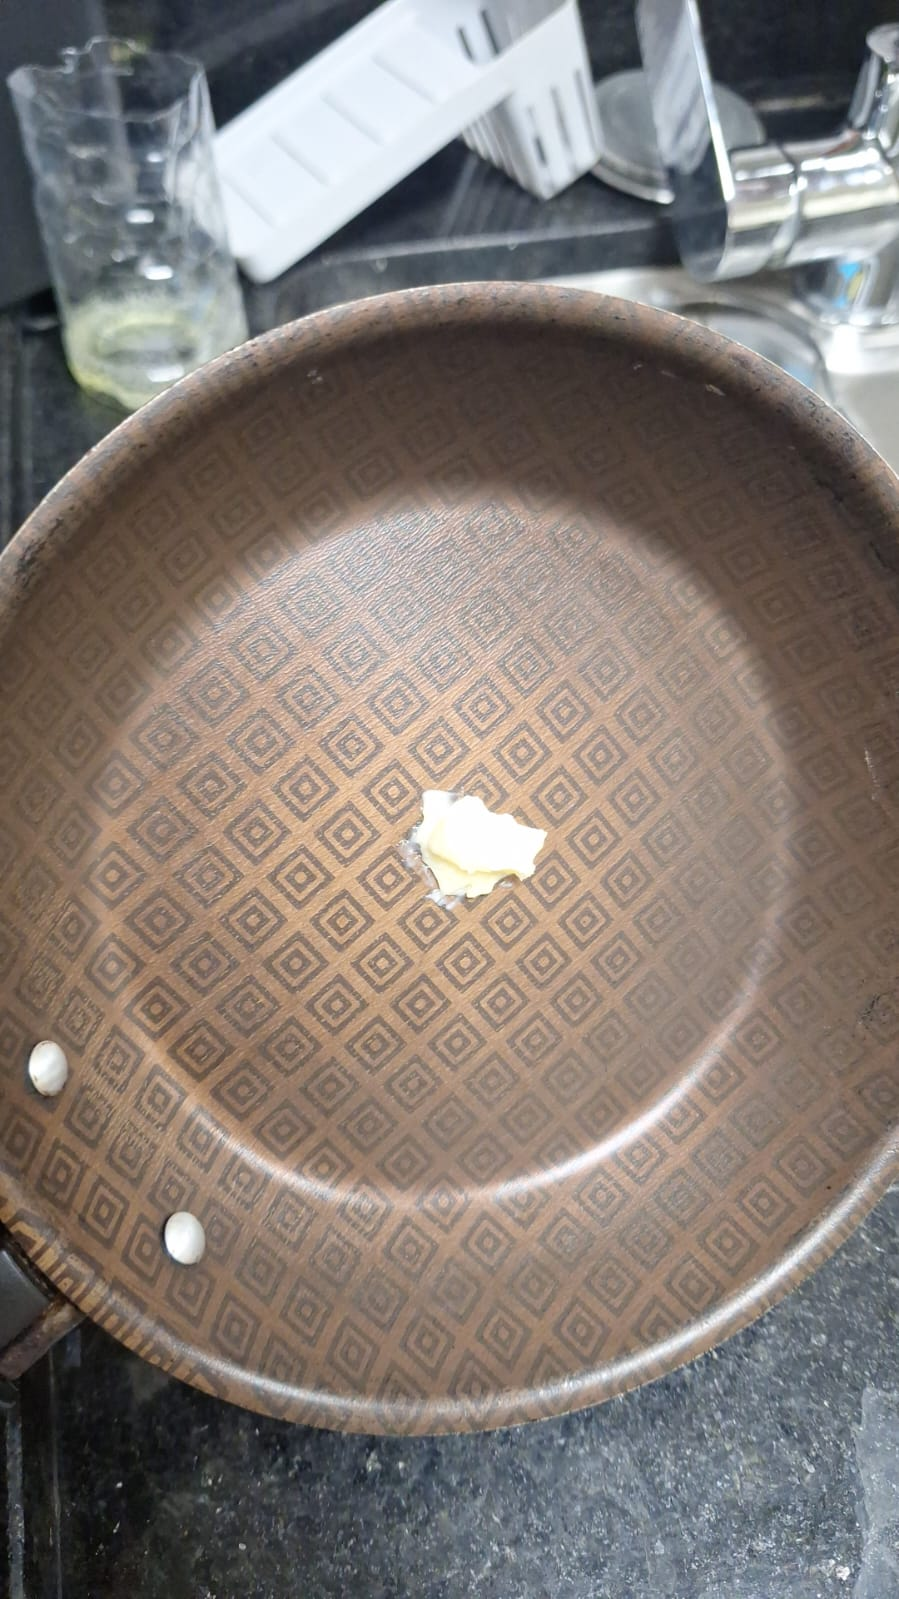
\includegraphics[width=0.4\textwidth]{src/fig/casa/porcao_manteiga.jpeg}
    \caption{Porção padronizada de manteiga utilizada no teste de limpeza.}
    \label{fig:limpeza_manteiga}
\end{figure}

Os resultados obtidos para cada amostra são apresentados na Figura~\ref{fig:limpeza_resultados}. O sabão da quinta aula destacou-se entre todos, sendo o que melhor dissolveu a manteiga na água — resultado coerente com a sua avaliação como o melhor produto do conjunto.

\begin{figure}[H]
    \centering
    \begin{subfigure}{0.45\textwidth}
        \centering
        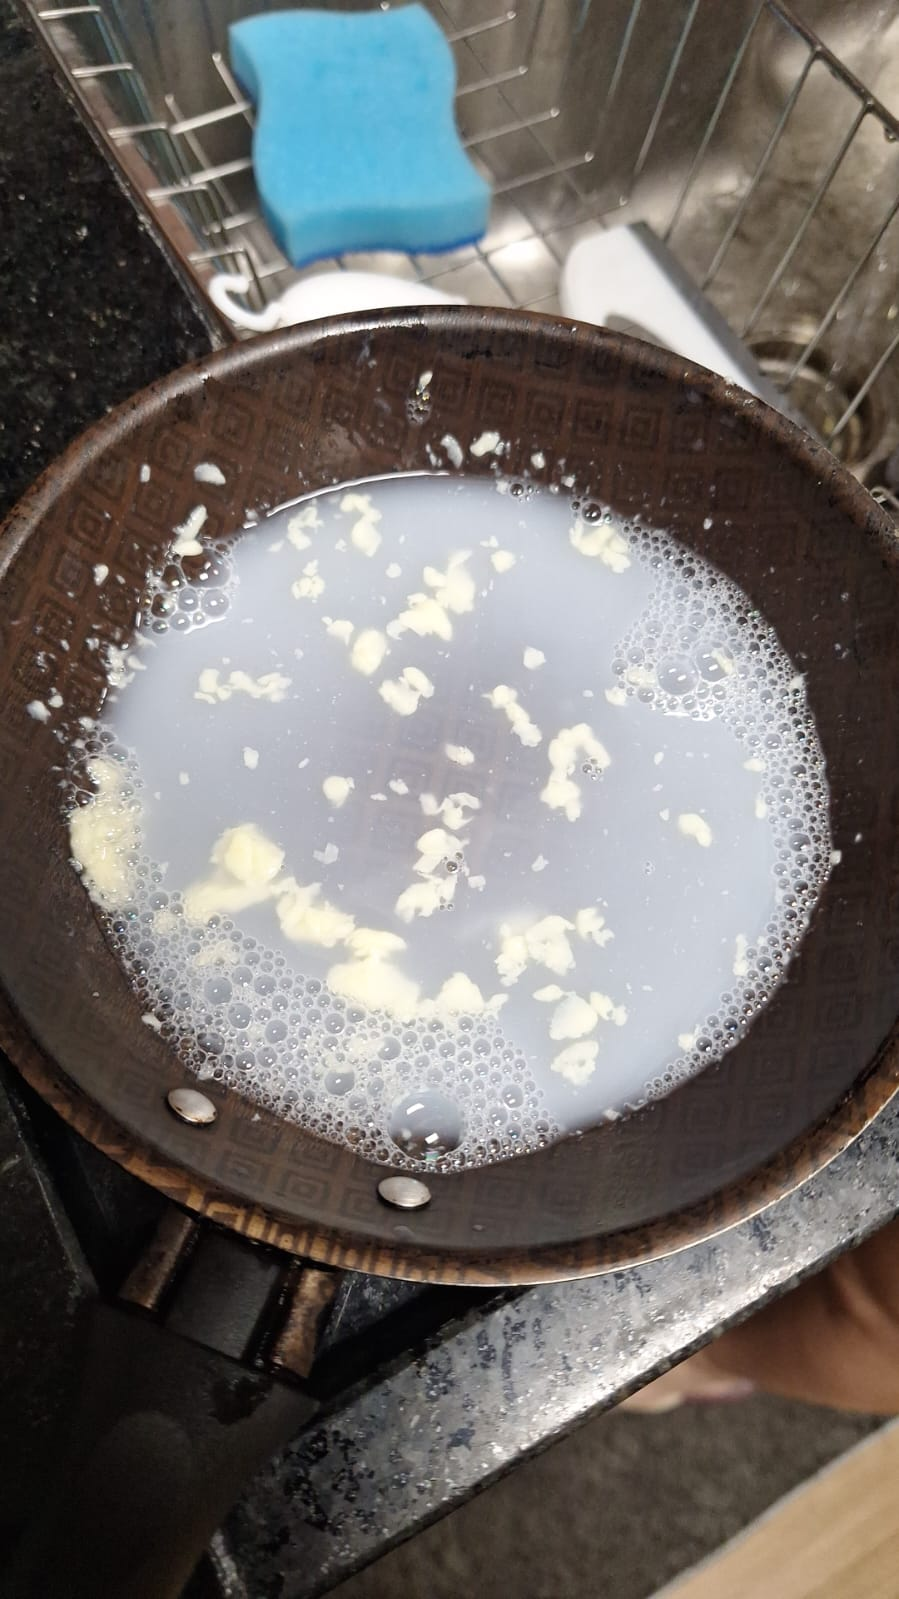
\includegraphics[width=\textwidth]{src/fig/casa/limpeza_d1.jpeg}
        \caption{Dia 1}
    \end{subfigure}
    \hfill
    \begin{subfigure}{0.45\textwidth}
        \centering
        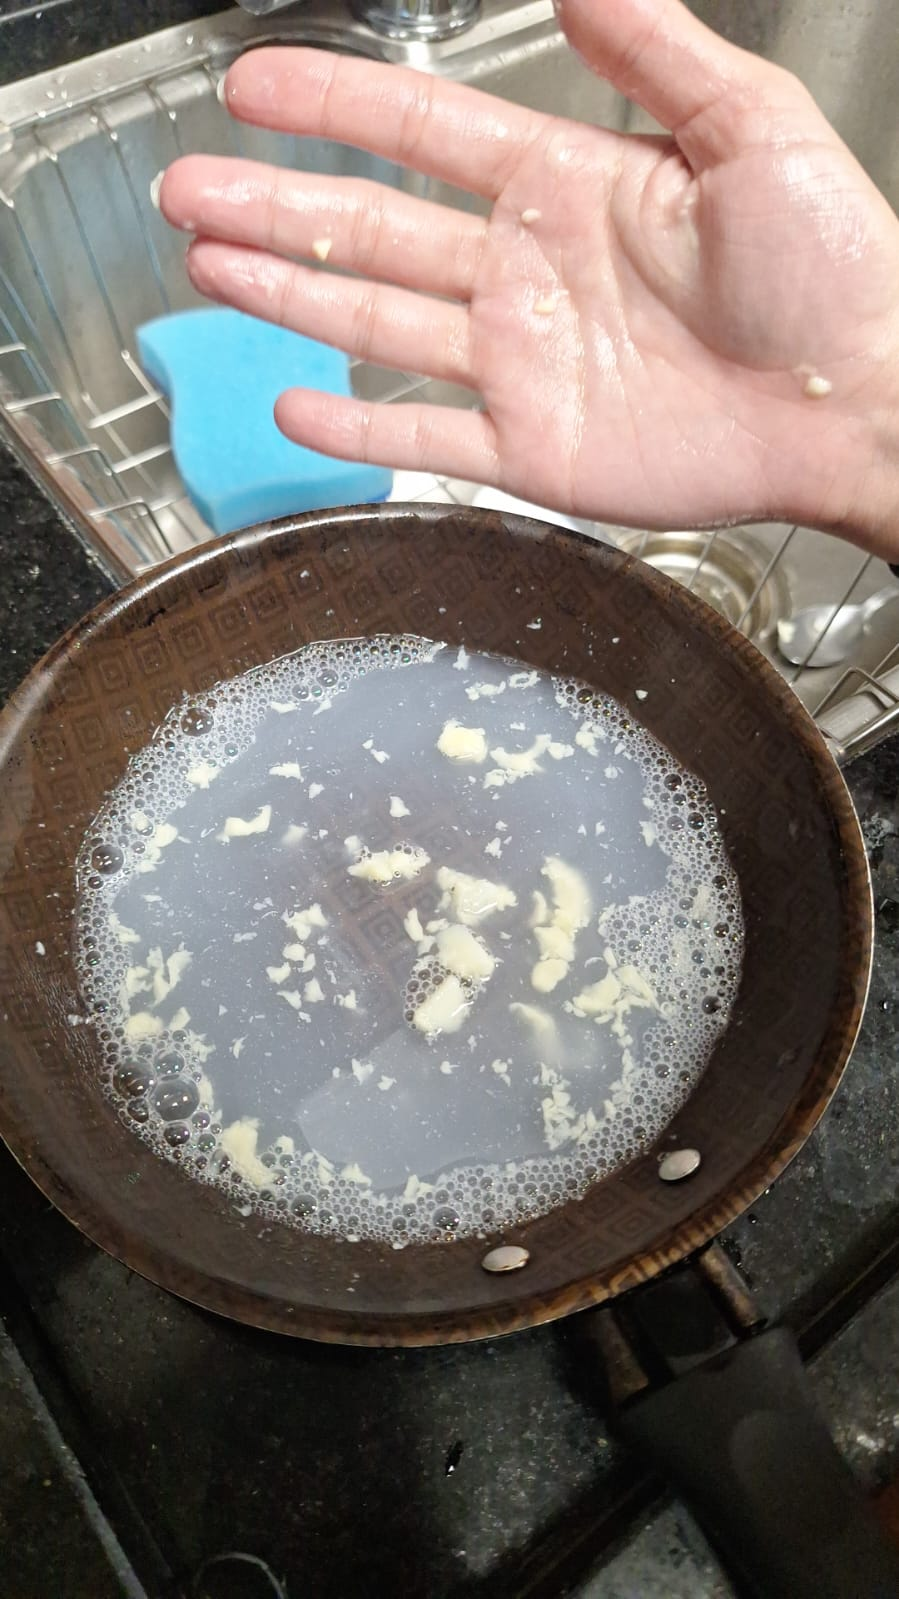
\includegraphics[width=\textwidth]{src/fig/casa/limpeza_d4.jpeg}
        \caption{Dia 4}
    \end{subfigure}

    \vspace{1ex}

    \begin{subfigure}{0.45\textwidth}
        \centering
        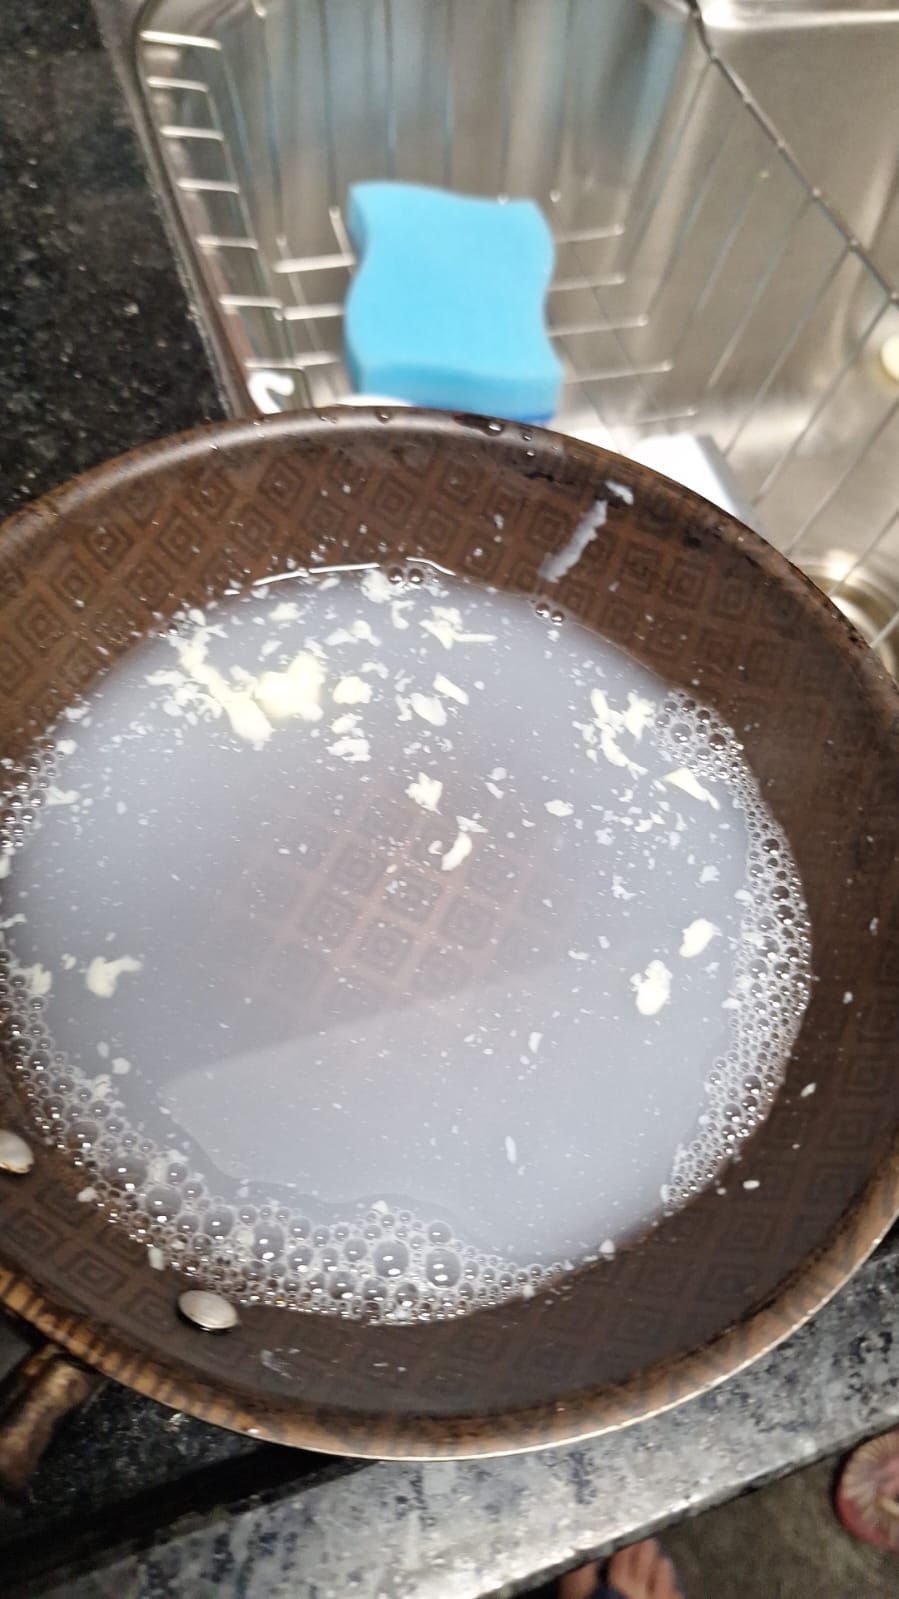
\includegraphics[width=\textwidth]{src/fig/casa/limpeza_d5.jpeg}
        \caption{Dia 5}
    \end{subfigure}
    \hfill
    \begin{subfigure}{0.45\textwidth}
        \centering
        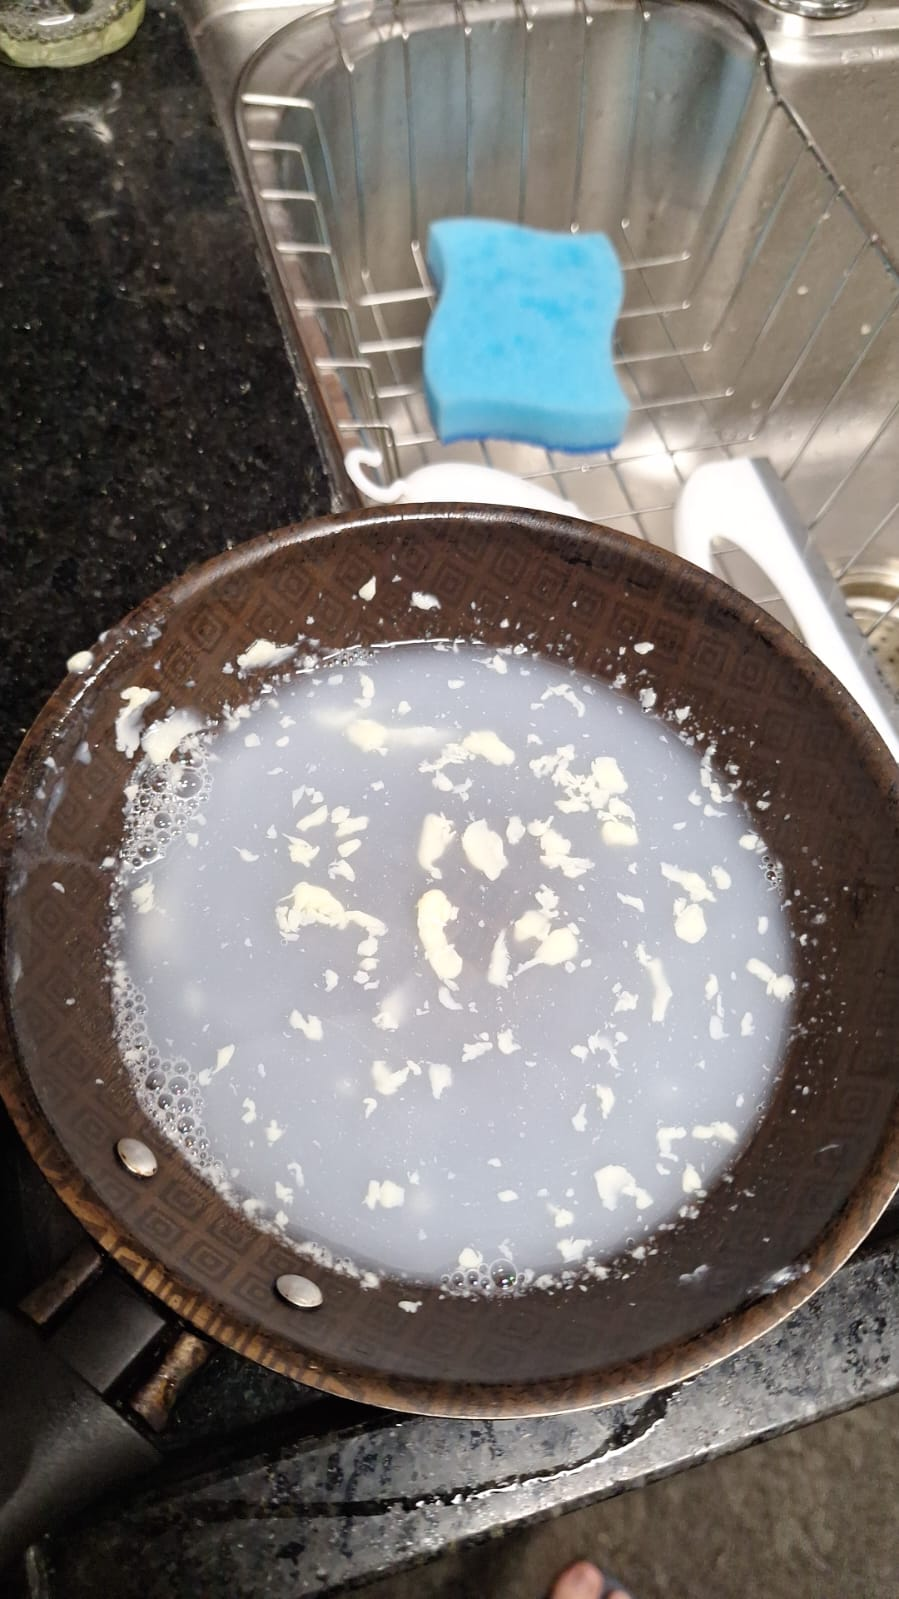
\includegraphics[width=\textwidth]{src/fig/casa/limpeza_d6.jpeg}
        \caption{Dia 6}
    \end{subfigure}
    \caption{Teste de limpeza com manteiga para as amostras das aulas 1, 4, 5 e 6.}
    \label{fig:limpeza_resultados}
\end{figure}
